% 150 câu đã gỡ khỏi ngân hàng (chuyen_dang) — chép lại vào file dạng để khôi phục

% từ: cau-hoi/lop10/0D1_Menh_de_Tap_hop/0D1-1-2_Tinh_dung_sai_cua_menh_de.tex
\begin{ex}%[0D1B1-2]%[ma:7c41a82b]
	Cho $a,b$ là hai  số tự nhiên. Mệnh đề nào sau đây \textbf{sai}?
	 \choice
		{Nếu $a,  b$ là các số lẻ thì $ab$ lẻ}
		{\True  Nếu $a$ chẵn và $b$ lẻ thì $ab$ lẻ}
		 {Nếu $a$ và $b$ lẻ thì $a+b$ chẵn}
		{Nếu  $a^2$ lẻ thì $a$ lẻ}
	\loigiai{Mệnh đề “Nếu $a$ chẵn và $b$ lẻ thì $ab$ lẻ”  sai vì tích của một số tự nhiên bất kì với một số tự nhiên chẵn là một số tự nhiên chẵn.}
\end{ex}

% từ: cau-hoi/lop10/0D2_BPT_va_he_BPT_bac_nhat_hai_an/0D2-1-2_Mien_nghiem_cua_BPT_bac_nhat_hai_an.tex
\begin{ex}%[0D2N1-2]%[ma:edc2ef6b]
	Phần  không bị gạch sọc trong hình vẽ bên dưới là miền nghiệm của bất phương trình nào?
	\begin{center}
		\begin{tikzpicture}[scale=.8,>=stealth,font=\footnotesize,line join=round,line cap=round]
				 \def\a{3/2} \def\b{3}
				\def\xmin{-4} \def\xmax{2} 
				\def\ymin{-1}  \def\ymax{4}
				\draw[->]  (\xmin,0)--(\xmax+.2,0) node [below]{$x$};
				 \draw[->] (0,\ymin)--(0,\ymax+.2) node [left]{$y$};
				\fill (0,0) circle (1pt) node[below left]{$O$}; 
				\clip (\xmin,\ymin) rectangle (\xmax,\ymax); 
				\fill[pattern=north west  lines]plot (\x,{\a*(\x)+\b})--(\xmin,\ymax)--(\xmin,\ymin)--cycle;
				 \draw[smooth,samples=300] plot (\x,{\a*(\x)+\b});
				\draw[fill=black] (0,3)  circle (1pt) node [right]{$3$};
				\draw[fill=black]  (-2,0) circle (1pt) node [below]{$-2$};
			\end{tikzpicture}
	\end{center}
	\choice 
		{$ 3x-2y<-6$} 
		{\True  $ 3x-2y>-6$}
		{$  3x-2y>0$}
		 {$ 3x-2y<0$}
	 \loigiai{
		Đường  thẳng $\Delta\colon ax+by=c$ đi qua hai điểm $\left(-2;0\right)$, $\left(0;3\right)$.\\
		Suy ra $\heva{&a\cdot(-2)+b\cdot0=c\\&a\cdot0+b\cdot3=c}\Rightarrow -2a=3b$.\\ 
		Chọn $\heva{&a=3\\&b=-2}\Rightarrow c=-6\Rightarrow \Delta\colon 3x-2y=-6$.\\ 
		Ta thấy điểm $\left(0;0\right)$ thuộc  miền nghiệm của bất phương trình (phần không gạch sọc).\\
		Do đó không phần  gạch sọc là miền nghiệm của bất phương trình $3x-2y>-6$.
	 }
\end{ex}

% từ: cau-hoi/lop10/0D2_BPT_va_he_BPT_bac_nhat_hai_an/0D2-1-2_Mien_nghiem_cua_BPT_bac_nhat_hai_an.tex
\begin{ex}%[0D2N1-2]%[ma:055195ee]
	Phần không bị gạch sọc trong hình  vẽ bên dưới là miền nghiệm của bất phương trình nào?
	\begin{center}
		\begin{tikzpicture}[scale=.8,>=stealth,font=\footnotesize,line join=round,line cap=round]
				\def\a{1/2} \def\b{-2} 
				\def\xmin{-2} \def\xmax{5} 
				 \def\ymin{-3} \def\ymax{2}
				\draw[->] (\xmin,0)--(\xmax+.2,0) node  [below]{$x$};
				\draw[->]  (0,\ymin)--(0,\ymax+.2) node [left]{$y$};
				\fill (0,0)  circle (1pt) node[below left]{$O$};
				\clip  (\xmin,\ymin) rectangle (\xmax,\ymax);
				\fill[pattern=north west  lines] (\xmax,\ymax)--(\xmin,\ymax)--plot (\x,{\a*(\x)+\b})--(5,.5)--cycle;
				\draw[smooth,samples=300] plot (\x,{\a*(\x)+\b}); 
				\draw[fill=black] (0,-2) circle (1pt) node  [below right]{$-2$};
				\draw[fill=black] (4,0) circle (1pt)  node [below]{$4$};
			\end{tikzpicture}
	\end{center}
	 \choice
		{$2x-4y<8$} 
		 {\True $2x-4y>8$}
		{$2x-4y>-5$} 
		 {$2x-4y>-3$}
	\loigiai{ 
		Đường thẳng $\Delta\colon ax+by=c$ đi qua hai điểm $\left(4;0\right)$,  $\left(0;-2\right)$.\\
		Suy  ra $\heva{&a\cdot4+b\cdot0=c\\&a\cdot0+b\cdot(-2)=c}\Rightarrow 4a=-2b$.\\
		Chọn  $\heva{&a=2\\&b=-4}\Rightarrow c=8\Rightarrow \Delta\colon 2x-8y=8$.\\
		Ta  thấy điểm $\left(0;0\right)$ không thuộc miền nghiệm của bất phương trình (phần gạch sọc).\\
		Do đó không phần gạch sọc là miền nghiệm của bất phương trình $2x-8y>8$. 
	 }
\end{ex}

% từ: cau-hoi/lop10/0D2_BPT_va_he_BPT_bac_nhat_hai_an/0D2-1-2_Mien_nghiem_cua_BPT_bac_nhat_hai_an.tex
\begin{ex}%[0D2N1-2]%[ma:9019dca8]
	Phần bị gạch sọc trong hình vẽ bên dưới là miền nghiệm của bất phương trình  nào?\\
	\begin{center}
		\begin{tikzpicture}[scale=.8,>=stealth,font=\footnotesize,line join=round,line cap=round]
				 \def\a{2} \def\b{-3}
				\def\xmin{-2} \def\xmax{4} 
				\def\ymin{-4}  \def\ymax{2}
				 \draw[->] (\xmin,0)--(\xmax+.2,0) node [below]{$x$};
				\draw[->] (0,\ymin)--(0,\ymax+.2) node  [left]{$y$};
				\fill (0,0) circle (1pt)  node[below left]{$O$};
				\clip (\xmin,\ymin) rectangle (\xmax,\ymax); 
				\fill[pattern=north  west lines]plot (\x,{\a*(\x)+\b})--(\xmax,\ymax)--(\xmax,\ymin)--cycle;
				 \draw[smooth,samples=300] plot (\x,{\a*(\x)+\b});
				\draw[fill=black] (0,-3) circle (1pt) node [left]{$-3$}; 
				\draw[fill=black] (1.5,0)  circle (1pt) node [above]{$\dfrac{3}{2}$};
			\end{tikzpicture}
	\end{center}
	\choice 
		 {\True $ 2x-y>3$}
		 {$ 2x-y<3$}
		{$  x-2y<3$}
		{$  x-2y>3$}
	 \loigiai{
		Đường thẳng $\Delta\colon ax+b=c$ đi qua hai điểm $\left(\dfrac{3}{2};0\right)$, $\left(0;-3\right)$.\\ 
		Suy ra $\heva{&a\cdot\dfrac{3}{2}+b\cdot0=c\\&a\cdot0+b\cdot(-3)=c}\Rightarrow \dfrac{3}{2}a=-3b$.\\ 
		Chọn  $\heva{&a=2\\&b=-1}\Rightarrow c=3\Rightarrow \Delta\colon 2x-y=3$.\\
		Ta thấy điểm $\left(0;0\right)$ không thuộc miền nghiệm của bất phương trình (phần gạch sọc).\\ 
		Do đó  phần gạch sọc trong hình vẽ là miền nghiệm của bất phương trình $2x-y>3$.
	 }
\end{ex}

% từ: cau-hoi/lop10/0D2_BPT_va_he_BPT_bac_nhat_hai_an/0D2-2-2_Mien_nghiem_cua_He_BPT_bac_nhat_hai_an.tex
\begin{ex}%[0D2H2-2]%[ma:43393b88]
	Miền nghiệm của hệ bất phương trình $\heva{& x+y-1>0\\ & y\geq 2\\  &-x+2y>3}$ là phần \textbf{không} tô đậm của hình vẽ nào trong các hình vẽ sau?
	\choice 
		{\begin{tikzpicture}[line join=round,line cap=round,>=stealth,font=\footnotesize,scale=0.6]
		\draw (0,0)  node [below left] {$O$};
		\draw [->] (-3.5,0)--(3.5,0) node[below]{$x$}; 
		 \draw[->] (0,-3.5)--(0,3.5) node[left]{$y$};
		 \clip (-3.5,-3.5) rectangle (3.5,3.5);
		\foreach  \x in {-3,1}
		 \draw[shift={(\x,0)},color=black] (0pt,2pt) -- (0pt,-2pt) node[below] {\footnotesize $\x$};
		\foreach  \y in {1,2}
		 \draw[shift={(0,\y)},color=black] (2pt,0pt) -- (-2pt,0pt) node[left] {\footnotesize $\y$};
		\draw[samples=100,smooth,domain=-3.5:3.5,black]  plot (\x,{2});
		\draw[samples=100,smooth,domain=-3.5:3.5,black] plot  (\x,{1-(\x)});
		\draw[samples=100,smooth,domain=-3.5:3.5,black] plot  (\x,{0.5*(\x)+1.5});
		 \fill[pattern=north east lines,opacity=0.6] plot[domain=-3.5:3.5](\x,{1-(\x)})--plot[domain=3.5:-3.5](\x,{-3.5})--cycle;
		\fill[pattern=north  east lines,opacity=0.6] plot[domain=-3.5:3.5](\x,{2})--plot[domain=3.5:-3.5](\x,{-3.5})--cycle;
		 \fill[pattern=north east lines,opacity=0.6] plot[domain=-3.5:3.5](\x,{0.5*(\x)+1.5})--plot[domain=3.5:-3.5](\x,{3.5})--cycle;
	\end{tikzpicture}
		 }
		{\True\begin{tikzpicture}[line join=round,line cap=round,>=stealth,font=\footnotesize,scale=0.6]
		\draw (0,0) node [below  left] {$O$};
		\draw [->] (-3.5,0)--(3.5,0) node[below]{$x$}; 
		\draw[->]  (0,-3.5)--(0,3.5) node[left]{$y$};
		\clip (-3.5,-3.5) rectangle  (3.5,3.5);
		\foreach \x in  {-3,1}
		\draw[shift={(\x,0)},color=black] (0pt,2pt) --  (0pt,-2pt) node[below] {\footnotesize $\x$};
		\foreach \y in  {1,2}
		\draw[shift={(0,\y)},color=black] (2pt,0pt) -- (-2pt,0pt) node[left]  {\footnotesize $\y$};
		 \draw[samples=100,smooth,domain=-3.5:3.5,black] plot (\x,{2});
		 \draw[samples=100,smooth,domain=-3.5:3.5,black] plot (\x,{1-(\x)});
		\draw[samples=100,smooth,domain=-3.5:3.5,black] plot (\x,{0.5*(\x)+1.5}); 
		\fill[pattern=north  east lines,opacity=0.6] plot[domain=-3.5:3.5](\x,{1-(\x)})--plot[domain=3.5:-3.5](\x,{-3.5})--cycle;
		\fill[pattern=north east lines,opacity=0.6]  plot[domain=-3.5:3.5](\x,{2})--plot[domain=3.5:-3.5](\x,{-3.5})--cycle;
		\fill[pattern=north  east lines,opacity=0.6] plot[domain=-3.5:3.5](\x,{0.5*(\x)+1.5})--plot[domain=3.5:-3.5](\x,{-3.5})--cycle;
	\end{tikzpicture}
		 }
		{\begin{tikzpicture}[line join=round,line cap=round,>=stealth,font=\footnotesize,scale=0.6]
		\draw  (0,0) node [below left] {$O$};
		\draw [->] (-3.5,0)--(3.5,0)  node[below]{$x$};
		\draw[->]  (0,-3.5)--(0,3.5) node[left]{$y$};
		 \clip (-3.5,-3.5) rectangle (3.5,3.5);
		\foreach \x in  {-3,1}
		\draw[shift={(\x,0)},color=black] (0pt,2pt)  -- (0pt,-2pt) node[below] {\footnotesize $\x$};
		\foreach \y in  {1,2}
		\draw[shift={(0,\y)},color=black] (2pt,0pt) -- (-2pt,0pt) node[left] {\footnotesize $\y$}; 
		\draw[samples=100,smooth,domain=-3.5:3.5,black]  plot (\x,{2});
		\draw[samples=100,smooth,domain=-3.5:3.5,black] plot (\x,{1-(\x)}); 
		\draw[samples=100,smooth,domain=-3.5:3.5,black] plot  (\x,{0.5*(\x)+1.5});
		\fill[pattern=north east lines,opacity=0.6] plot[domain=-3.5:3.5](\x,{1-(\x)})--plot[domain=3.5:-3.5](\x,{3.5})--cycle; 
		\fill[pattern=north  east lines,opacity=0.6] plot[domain=-3.5:3.5](\x,{2})--plot[domain=3.5:-3.5](\x,{-3.5})--cycle;
		\fill[pattern=north  east lines,opacity=0.6] plot[domain=-3.5:3.5](\x,{0.5*(\x)+1.5})--plot[domain=3.5:-3.5](\x,{-3.5})--cycle;
	\end{tikzpicture}
		} 
		{\begin{tikzpicture}[line join=round,line cap=round,>=stealth,font=\footnotesize,scale=0.6]
		 \draw (0,0) node [below left] {$O$};
		\draw [->] (-3.5,0)--(3.5,0)  node[below]{$x$};
		\draw[->]  (0,-3.5)--(0,3.5) node[left]{$y$};
		\clip (-3.5,-3.5) rectangle (3.5,3.5); 
		\foreach \x in  {-3,1}
		\draw[shift={(\x,0)},color=black] (0pt,2pt) -- (0pt,-2pt) node[below]  {\footnotesize $\x$};
		\foreach \y in  {1,2}
		 \draw[shift={(0,\y)},color=black] (2pt,0pt) -- (-2pt,0pt) node[left] {\footnotesize $\y$};
		 \draw[samples=100,smooth,domain=-3.5:3.5,black] plot (\x,{2});
		\draw[samples=100,smooth,domain=-3.5:3.5,black] plot  (\x,{1-(\x)});
		\draw[samples=100,smooth,domain=-3.5:3.5,black] plot (\x,{0.5*(\x)+1.5}); 
		\fill[pattern=north east  lines,opacity=0.6] plot[domain=-3.5:3.5](\x,{1-(\x)})--plot[domain=3.5:-3.5](\x,{3.5})--cycle;
		\fill[pattern=north east lines,opacity=0.6]  plot[domain=-3.5:3.5](\x,{2})--plot[domain=3.5:-3.5](\x,{3.5})--cycle;
		 \fill[pattern=north east lines,opacity=0.6] plot[domain=-3.5:3.5](\x,{0.5*(\x)+1.5})--plot[domain=3.5:-3.5](\x,{-3.5})--cycle;
	\end{tikzpicture}
		} 
	\loigiai{ 
		Chọn điểm $(0;3)$ là điểm nằm trong miền nghiệm hệ bất phương trình. Do đó ta chọn  hình
		\begin{center}
			\begin{tikzpicture}[line join=round,line cap=round,>=stealth,font=\footnotesize,scale=0.6]
					\draw (0,0) node [below left]  {$O$};
					 \draw [->] (-3.5,0)--(3.5,0) node[below]{$x$};
					\draw[->] (0,-3.5)--(0,3.5)  node[left]{$y$};
					\clip (-3.5,-3.5) rectangle (3.5,3.5); 
					\foreach \x in  {-3,1}
					\draw[shift={(\x,0)},color=black]  (0pt,2pt) -- (0pt,-2pt) node[below] {\footnotesize $\x$};
					\foreach \y in {1,2} 
					\draw[shift={(0,\y)},color=black] (2pt,0pt) -- (-2pt,0pt)  node[left] {\footnotesize $\y$};
					 \draw[samples=100,smooth,domain=-3.5:3.5,black] plot (\x,{2});
					\draw[samples=100,smooth,domain=-3.5:3.5,black]  plot (\x,{1-(\x)});
					\draw[samples=100,smooth,domain=-3.5:3.5,black] plot (\x,{0.5*(\x)+1.5}); 
					\fill[pattern=north  east lines,opacity=0.6] plot[domain=-3.5:3.5](\x,{1-(\x)})--plot[domain=3.5:-3.5](\x,{-3.5})--cycle;
					\fill[pattern=north  east lines,opacity=0.6] plot[domain=-3.5:3.5](\x,{2})--plot[domain=3.5:-3.5](\x,{-3.5})--cycle;
					\fill[pattern=north east lines,opacity=0.6]  plot[domain=-3.5:3.5](\x,{0.5*(\x)+1.5})--plot[domain=3.5:-3.5](\x,{-3.5})--cycle;
				\end{tikzpicture}
		\end{center}
	 }
\end{ex}

% từ: cau-hoi/lop10/0D2_BPT_va_he_BPT_bac_nhat_hai_an/0D2-2-3_Toan_thuc_te_ve_He_BPT_bac_nhat_hai_an.tex
\begin{bt}%[0D2V2-3] % KIEM_TRA%[Dự án đề kiểm tra HKI NH22-23- Nguyễn Ngọc Nguyên]%[THPT Trưng Vương]%[ma:7bb0dded]
	\textbf{Bài toán về \lq\lq Đặt ghế VIP trong rạp chiếu phim\rq\rq:}\\
	\immini{Tại một phòng chiếu phim, màn hình có chiều ngang $18$ mét. Người ta thiết kế ghế VIP tại vị trí mà khán giả có góc quan sát lý tưởng nhất. Giả sử rằng góc quan sát lý tưởng nhất của khán giả đến màn hình từ $50^\circ$ đến $58^\circ$. Tính khoảng cách từ màn hình đến vị trí có thể đặt ghế VIP trong phòng chiếu phim, biết rằng ghế VIP đặt chính giữa màn hình (kết quả làm tròn đến hàng phần trăm).}
	{	\begin{tikzpicture}[scale=.9, font=\footnotesize, line join=round, line cap=round, >=stealth]
			\path
			(0,0) coordinate (A)node[left]{Ghế VIP}
			(6,3) coordinate (B)
			(6,-3)coordinate (C)
			(6,0)node[right]{Màn hình}
			(1,0)node[right] {Góc quan sát}
			;
			\draw[line width=2mm](B)--(C);
			\draw 
			(B)--(A)--(C)
			pic[angle radius=9mm,draw=blue,fill=green!50,opacity=.3] {angle = C--A--B}
			;
			%\foreach \p/\g in {A/180,B/90,H/0,C/-90} \draw[fill=black](\p)circle(.04)node[shift={(\g:.25)}]{$\p$};
			
	\end{tikzpicture}}
	\loigiai{
		\immini{Gọi $BC$ là chiều ngang của màn hình, $A$ là vị trí đặt ghế VIP và $H$ là trung điểm $BC$ như hình bên.\\
		 Do đó $AH$ là khoảng cách từ màn hình đến ghế VIP.\\
		 Suy ra $AH\perp BC$ tại $H$ và $\widehat{BAC}$ là góc quan sát lý tưởng.\\
	 	 Khi đó $BC=18$ mét, $BH=9$ mét và $\widehat{BAH}=\dfrac{1}{2}\widehat{BAC}$.
		\begin{itemize}
			\item Trường hợp  $\widehat{BAC}=58^\circ$\\
				 Xét $\triangle AHB$ vuông tại H, có $\tan\widehat{BAH}=\dfrac{BH}{AH}$\\
				 $\Rightarrow AH=\dfrac{BH}{\tan 29^\circ}=\dfrac{9}{\tan 29^\circ}\approx 16{,}24$ mét.
			\item Trường hợp  $\widehat{BAC}=50^\circ$\\
				Xét $\triangle AHB$ vuông tại H, có
				$\tan\widehat{BAH}=\dfrac{BH}{AH}$\\
				$\Rightarrow AH=\dfrac{BH}{\tan 25^\circ}=\dfrac{9}{\tan 25^\circ}\approx 19{,}30$ mét.
		\end{itemize}}
			{\begin{tikzpicture}[scale=1, font=\footnotesize, line join=round, line cap=round, >=stealth]
				\path
				(0,0) coordinate (A)
				(6,3) coordinate (B)
				(6,-3)coordinate (C)
				(6,0) coordinate (H)
				;
				\draw (A)--(B)--(C)--cycle (A)--(H);
				
				\foreach \p/\g in {A/180,B/90,H/0,C/-90} \draw[fill=black](\p)circle(.04)node[shift={(\g:.25)}]{$\p$};
				
		\end{tikzpicture}}
		\noindent Vậy khoảng cách từ màn hình đến vị trí có thể đặt ghế VIP trong phòng chiếu phim trong khoảng $16{,}24$ mét đến $19{,}30$ mét.
		
	}
\end{bt}

% từ: cau-hoi/lop10/0D3_Ham_so_bac_hai_va_do_thi/0D3-1-4_Do_thi_cua_ham_so.tex
\begin{ex}%[0D3H1-4]%[ma:e4c54c1d]
	Cho hàm số ${y=f(x)}$ có  đồ thị là đường gấp khúc như hình bên dưới.
	\begin{center}
		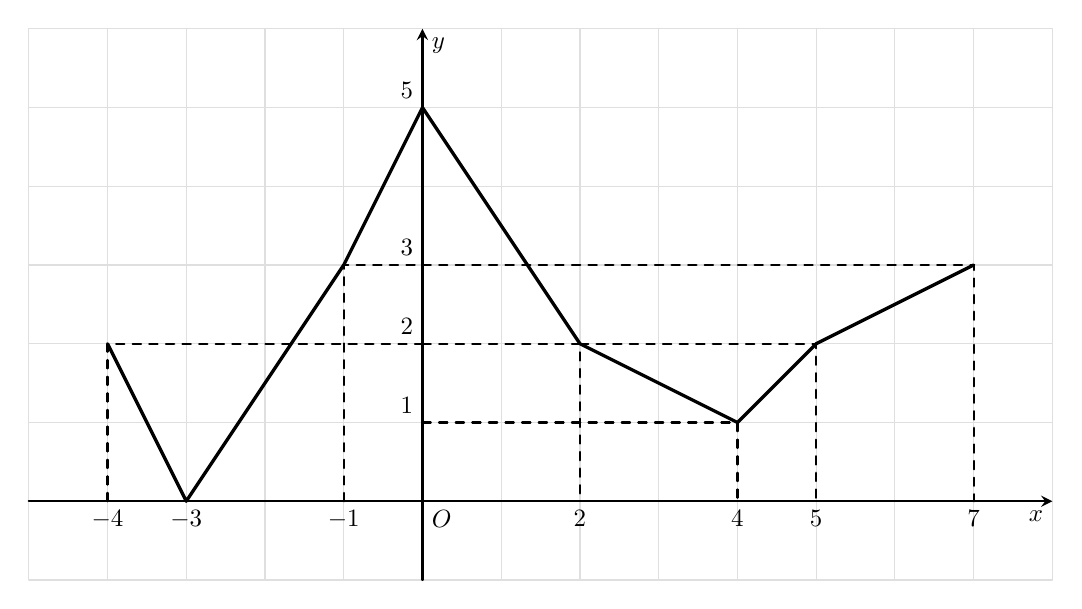
\begin{tikzpicture}[line join=round,line cap=round,thick]
				 \draw[gray!50,thin,opacity=.5]
					(-5,-1)  grid (8,6);
				\draw [-stealth,thick](-5,0) -- (8,0)  node[below left]{$x$};
				\draw  [-stealth,thick](0,-1) -- (0,6) node[below right]{$y$};
				\draw[very thick]  (-4,2)--(-3,0)--(-1,3)--(0,5)--(2,2)--(4,1)--(5,2)--(7,3);
				\draw[dashed] (-4,0) node[below]{$-4$}|-(0,2) node[above left]{$2$} 
					(-1,0) node[below]{$-1$}|-(0,3) node[above  left]{$3$}
					(0,2)-|(2,0) node[below]{$2$} 
					 (0,1) node[above left]{$1$}-|(4,0) node[below]{$4$}
					(2,2)--(5,2)--(5,0) node[below]{$5$} 
					(0,3)-|(7,0) node[below]{$7$} 
					(0,0) node[below right]{$O$} 
					 (-3,0) node[below]{$-3$}
					(0,5) node[above  left]{$5$};
			\end{tikzpicture}
	\end{center}
	Khi đó 
	\choiceTF 
		{Tập giá trị hàm số  $T=[-4;7]$}
		{\True Ta thấy điểm $(-4;2)$, $(4;1)$ thuộc đồ thị hàm số, điểm $(2;3)$ không thuộc đồ thị hàm  số}
		{\True Ta  có $f(-1)=3$, $f(5)=2$}
		{\True Hàm số đã  cho đồng biến trên các khoảng $(-3;0)$, $(4;7)$; hàm số nghịch biến trên các khoảng $(-4;-3)$, $(0;4)$}
	\loigiai{ 
		\begin{itemchoice}
			\itemch Tập xác định hàm  số $\mathscr{D}=[-4;7]$. Tập giá trị hàm số $T=[0;5]$.
			\itemch Ta thấy điểm $(-4;2)$, $(4;1)$  thuộc đồ thị hàm số, điểm $(2;3)$ không thuộc đồ thị hàm số.
			\itemch Ta có  $f(-1)=3$, $f(5)=2$.
			\itemch Hàm số đã cho đồng biến trên các khoảng $(-3;0)$, $(4;7)$; hàm số nghịch biến trên  các khoảng $(-4;-3)$, $(0;4)$.
		\end{itemchoice}
	} 
\end{ex}

% từ: cau-hoi/lop10/0D3_Ham_so_bac_hai_va_do_thi/0D3-1-5_Tinh_dong_bien_nghich_bien.tex
\begin{bt}%[0D3H1-5]%[Dự án đề kiểm tra Toán 10 GHKI NH23-24- Nguyễn Trần Phong]%[THPT NTMK - Tp HCM]%[ma:c4959ce7]
	Xét tính đồng biến, nghịch biến của hàm số $y=f(x)=x^2 -2$ trên khoảng $(-\infty; 0)$ bằng định nghĩa.
	\loigiai{
		Với mọi $x_1$, $x_2 \in (-\infty; 0) \colon x_1 > x_2 \Leftrightarrow x_1 -x_2 >0$, ta có 
		$$f(x_1) - f(x_2) = x_1^2 -x_2^2 = (x_1-x_2) \cdot (x_1+x_2).$$
		Do $x_1$, $x_2 \in (-\infty; 0)$ và $x_1 -x_2>0$ nên $(x_1-x_2) \cdot (x_1+x_2) <0$.\\
		Suy ra $f(x_1) < f(x_2)$ với mọi $x_1$, $x_2 \in (-\infty; 0)$.\\
		Vậy hàm số đã cho nghịch biến trên khoảng $(-\infty; 0)$}
\end{bt}

% từ: cau-hoi/lop10/0D3_Ham_so_bac_hai_va_do_thi/0D3-1-5_Tinh_dong_bien_nghich_bien.tex
\begin{bt}%[0D3H1-5]%[ma:c3b0e5c3]
	Cho hàm số $y=x^2-3x-10$. Chứng tỏ hàm số đã cho:
	\begin{listEX}[1]
		\item Nghịch biến trên khoảng $\left(-\infty;\dfrac{3}{2}\right)$;
		\item Đồng biến trên khoảng $\left(\dfrac{3}{2};+\infty\right)$.
	\end{listEX}
	\loigiai{
		Tập xác định $D=\mathbb{R}$. \\
		Với mọi $x_1, x_2 \in D$ và $x_1 < x_2$, ta xét:
		\begin{eqnarray*}
			f(x_1)-f(x_2)&=&(x^2_1-3x_1-10)-(x^2_2-3x_2-10)\\&=&(x^2_1-x^2_2)-3(x_1-x_2)\\&=&(x_1-x_2)(x_1+x_2-3)
		\end{eqnarray*}
		$\Rightarrow \dfrac{f(x_1)-f(x_2)}{x_1-x_2}=x_1+x_2-3$. \\
		\begin{listEX}[1]
			\item Với mọi $x_1, x_2 \in \left(-\infty;\dfrac{3}{2}\right)$ và $x_1 < x_2$ ta có: $\heva{& x_1 < \dfrac{3}{2} \\ & x_2 < \dfrac{3}{2}} \Rightarrow \dfrac{f(x_1)-f(x_2)}{x_1-x_2}=x_1+x_2-3 < 0$. \\
			Vậy hàm số nghịch biến trên khoảng $\left(-\infty;\dfrac{3}{2}\right)$.
			\item Với mọi $x_1, x_2 \in \left(\dfrac{3}{2};+\infty\right)$ và $x_1 < x_2$ ta có: $\heva{& x_1 > \dfrac{3}{2} \\ & x_2 > \dfrac{3}{2}} \Rightarrow \dfrac{f(x_1)-f(x_2)}{x_1-x_2}=x_1+x_2-3 > 0$. \\
			Vậy hàm số nghịch biến trên khoảng $\left(\dfrac{3}{2};+\infty\right)$.
		\end{listEX}
	}
\end{bt}

% từ: cau-hoi/lop10/0D3_Ham_so_bac_hai_va_do_thi/0D3-1-5_Tinh_dong_bien_nghich_bien.tex
\begin{bt}%[0D3H1-5]%[ma:083e7f36]
	Vẽ đồ thị của hàm số $y=3x+1$ và $y=-2x^2$. Hãy cho biết:
	\begin{listEX}[1]
		\item Hàm số $y=3x+1$ đồng biến hay nghịch biến trên $\mathbb{R}$.
		\item Hàm số $y=-2x^2$ đồng biến hay nghịch biến trên mỗi khoảng $(-\infty;0)$ và $(0;+\infty)$.
	\end{listEX}
	\loigiai{
		Đồ thị hàm số $y=3x+1$ và $y=-2x^2$.
		\begin{center}
			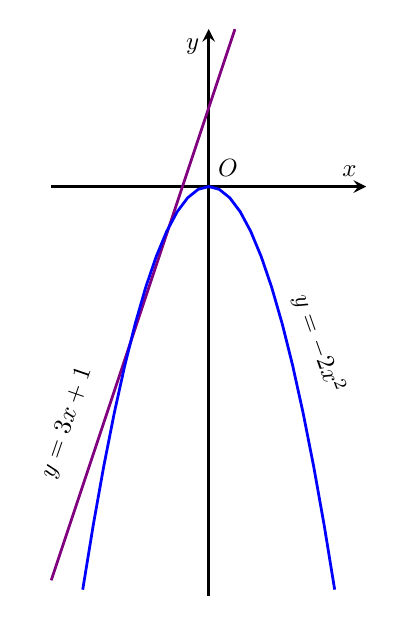
\begin{tikzpicture}[>=stealth]
			\draw[->,line width=1pt] (-2,0)--(0,0)node[above right]{$O$} --(2,0)node[above left]{$x$};
			\draw[->,line width=1pt] (0,-5.2)--(0,2)node[below left]{$y$};
			\draw[violet,line width=1pt] plot[domain=-2:1/3] (\x,{3*\x+1});
			\draw[blue,line width=1pt] plot[domain=-1.6:1.6] (\x,{-2*(\x)^2});
			\node at (1.4,-2)[rotate=-70.5]{$y=-2x^2$};
			\node at (-1.8,-3)[rotate=71]{$y=3x+1$};
			\end{tikzpicture}
		\end{center}
		\begin{listEX}[1]
			\item Đồ thì hàm số là đường đi lên từ trái sang phải nên hàm số đồng biến trên $\mathbb{R}$.
			\item Trên khoảng $(-\infty;0)$ hàm số đồng biến (đường đồ thị đi lên). \\
			Trên khoảng $(0;+\infty)$ hàm số nghịch biến (đường đồ thị đi xuống).
		\end{listEX}
	}
\end{bt}

% từ: cau-hoi/lop10/0D3_Ham_so_bac_hai_va_do_thi/0D3-2-1_Xac_dinh_ham_so_bac_hai.tex
\begin{ex}%[0D3N2-1]%[ma:5bb14943]
	\immini[thm]{Hàm  số nào sau đây có đồ thị như hình dưới đây?
	\choice 
		 {$y=x^2-3x+1$}
		{$y=-x^2+3x-1$} 
		{$y=-2x^2+3x-1$} 
		{\True$y=2x^2-3x+1$} 
		} 
		{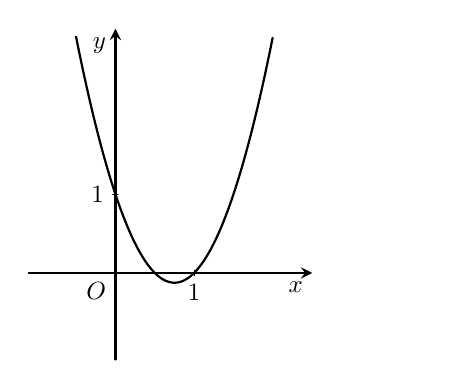
\begin{tikzpicture}[line join=round,line cap=round,>=stealth,thick]
		\tikzset{every  node/.style={scale=0.9}}
		 \draw[->] (-1.1,0)--(2.5,0) node[below left] {$x$};
		\draw[->] (0,-1.1)--(0,3.1)  node[below left] {$y$};
		\draw (0,0) node [below  left] {$O$};
		\foreach \x/\nx in {1/1} 
		 \draw[thin] (\x,1pt)--(\x,-1pt) node [below] {$\nx$};
		 \foreach \y/\ny in {1/1}
		 \draw[thin] (1pt,\y)--(-1pt,\y) node [left] {$\ny$};
		\begin{scope}
			\clip (-1,-1)  rectangle (4,3);
			\draw[samples=200,domain=-1:2,smooth,variable=\x] plot (\x,{2*(\x)^2+-3*(\x)+1}); 
		\end{scope}
	\end{tikzpicture}
		} 
	 \loigiai{
		Bề lõm  của parabol hướng lên trên suy ra $a>0$.\\
		Suy ra  loại đáp án $y=-x^2+3x-1$ và $y=-2x^2+3x-1$.\\
		Đồ thị đi qua điểm $(1; 0)$ nên  chọn $y=2x^2-3x+1$.
	} 
\end{ex}

% từ: cau-hoi/lop10/0D3_Ham_so_bac_hai_va_do_thi/0D3-2-1_Xac_dinh_ham_so_bac_hai.tex
\begin{bt}%[0D3H2-1]%[ma:5c61f42f]
Cho hàm số $y=f(x)=a x^2+b x+c$ có đồ thị như hình vẽ
\begin{center}
\begin{tikzpicture}[line join = round, line cap = round,>=stealth,font=\footnotesize,scale=0.7]
\def\xmin{-1.5} \def\xmax{4.5}
\def\ymin{-1.5} \def\ymax{4.5}
\foreach \x in {2} \draw (\x,2pt)--(\x,-2pt) node [above] {$\x$};
\draw[-stealth] (\xmin,0)--(\xmax,0)node[below]{$x$};
\foreach \y in {-1,3} \draw (2pt,\y)--(-2pt,\y) node [left] {$\y$};
\draw[-stealth] (0,\ymin)--(0,\ymax)node[right]{$y$};
\filldraw (0,0)node[below left]{$O$} circle (1.5pt);
\clip (\xmin,\ymin) rectangle (\xmax,\ymax);
\draw[samples=100,domain=\xmin:\xmax,smooth] plot (\x, {(\x)^2-4*(\x)+3});
\draw[dashed](0,-1)--(2,-1)--(2,0);
\end{tikzpicture}
\end{center}
\begin{listEX}
\item Tìm $a$, $b$, $c$.
\item Tìm giá trị lớn nhất và giá trị nhỏ nhất của hàm số đã cho trên đoạn $[0;3]$.
\end{listEX}
\loigiai{
\begin{listEX}
	\item Tìm $a$, $b$, $c$.
	\\
	Gọi $ (P) $ là đồ thị của hàm số đã cho. Dựa vào đồ thị trên, ta thấy $ (P) $ là parabol có đỉnh $ I(2;-1) $ và đi qua điểm $ M(0;3) $ nên ta có hệ phương trình
	$$
		\heva{
		&\dfrac{-b}{2a} = 2\\
		&4a+2b+c=-1\\
		&c=3
		}
		\Leftrightarrow
		\heva{
		&4a+b=0\\
		&4a+2b=-4\\
		&c=3
		}
		\Leftrightarrow
		\heva{
		&a=1\\
		&b=-4\\
		&c=3
		}
	$$
	Vậy $a=1$, $b=-4$ và $c=3$.
	\item Tìm giá trị lớn nhất và giá trị nhỏ nhất của hàm số đã cho trên đoạn $[0;3]$.
	\\
	Dựa vào đồ thị hàm số $ (P) $, ta thấy trên đoạn $ \left[ 0;3 \right] $
	$$
		\heva{
		&y_\text{max} = 3 \quad &\text{khi } x=0
		\\
		&y_\text{min} = -1 \quad &\text{khi } x=2
		}
	$$
\end{listEX}
}
\end{bt}

% từ: cau-hoi/lop10/0D3_Ham_so_bac_hai_va_do_thi/0D3-2-3_Do_thi_cua_ham_so_bac_hai.tex
\begin{ex}%[0D3H2-3]%[ma:90fe15f4]
	\immini{ 
	Cho hàm số $y=f(x)=a x^2+b x+c$  có đồ thị như hình vẽ. Đặt $\Delta=b^2-4ac$, tìm dấu của $a$ và $\Delta$.}
	{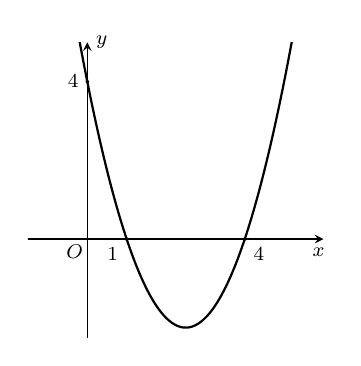
\begin{tikzpicture}[scale=0.5,font=\footnotesize,line join=round,
			line cap=round,>=stealth] 
		\def \xmin{-1.5} 
		\def  \xmax{6}
		\def  \ymin{-2.5}
		 \def \ymax{5}
		\draw[->] (\xmin,0)--(\xmax,0) node[shift=(-110:0.2)]  {$x$};
		\draw[->] (0,\ymin)--(0,\ymax)  node[right] {$y$};
		\fill  (0,0) circle (1pt) node[shift=(-135:0.25)]{$O$};
		\clip (\xmin,\ymin) rectangle (\xmax,\ymax); 
		\draw[smooth,samples=100,domain=\xmin:\xmax,thick] plot (\x,{(\x)^2-5*(\x)+4}); 
		 \foreach \x/\nx in {1/1}
		\draw (\x,0) circle (1pt) node[below left] {$\nx$}; 
		\foreach  \x/\nx in {4/4}
		\draw (\x,0) circle  (1pt) node[below right] {$\nx$};
		\foreach \y/\ny in {4/4} 
		\draw  (0,\y) circle (1pt) node[left] {$\ny$};
	\end{tikzpicture}
	} 
	\choice 
		{\True  $a>0$, $\Delta>0$}
		{$a<0$,  $\Delta>0$}
		{$a>0$, $\Delta=0$} 
		{$a<0$,  $\Delta=0$}
	\loigiai{ 
		Đồ thị hàm số là một parabol có bề lõm quay lên nên $a>0$ và đồ thị hàm số cắt trục $Ox$ tại hai điểm phân  biệt nên $\Delta>0$.
	} 
\end{ex}

% từ: cau-hoi/lop10/0D3_Ham_so_bac_hai_va_do_thi/0D3-2-6_Toan_thuc_te_ung_dung_ham_so_bac_hai.tex
\begin{bt}%[0D3V2-6]%[ma:3fe003fb]
	Bác Hùng dùng $40$ m lưới thép gai rào thành một mảnh vườn hình chữ nhật để trồng rau. Tính chu vi của mảnh vườn hình chữ nhật có diện tích lớn nhất mà bác Hùng có thể rào được (đơn vị: mét).
	\shortans[]{$40$}
	\loigiai{
		Bác Hùng dùng lưới để rào thành một mảnh vườn hình chữ nhật có chiều rộng $x$ (mét) như sau:
		\begin{center}
			\begin{tikzpicture}[line join=round, line cap=round,thick]
				\coordinate (A) at (0,3);
				\coordinate (B) at (5,3);
				\coordinate (D) at (0,0);
				\coordinate (C) at ($(B)+(D)-(A)$);
				\draw(A)--(B)--(C)--(D)--cycle;
				\path (A)--(D) node[midway, left]{$x$}
					  (B)--(C) node[midway, right]{$x$}
				;
				\foreach \i/\g in {A/90,B/90,C/-90,D/-90}{\draw[fill=black](\i) circle (1.0pt) ($(\i)+(\g:3mm)$) node[scale=1]{$\i$};}
			\end{tikzpicture}
		\end{center}
		Vì tấm lưới dài $40$ m, hay chính là chu vi của mảnh vườn hình chữ nhật $ABCD$ là $40$ m.\\
		Suy ra nửa chu vi của mảnh vườn là $40:2=20$\,(m).\\
		Do đó chiều dài của mảnh vườn rào được theo chiều rộng $x$\,(mét) là $20-x$\,(m).\\
		Diện tích mảnh vườn hình chữ nhật rào được theo chiều rộng $x$ (mét) là 
		$$S(x)=x\cdot (20-x)=-x^2+20x\,(\text{m}^2).$$
		Để tìm diện tích lớn nhất của mảnh vườn hình chữ nhật bác Hùng có thể rào được, ta tính giá trị lớn nhất của hàm số $S(x)$, đây là hàm số bậc hai.\\
		Tọa độ đỉnh của đồ thị hàm số bậc hai $S(x)=-x^2+20x$ là $I(10;100)$.\\ 
		Do đó giá trị lớn nhất của hàm số $S(x)$ là $S=100$ tại $x=10$.\\ 
		Suy ra chiều dài khi chiều rộng $x=10$\,m là $20-10=10$ (m).
		Vậy chu vi của mảnh vườn có diện tích lớn nhất là $4\cdot 10=40$ (m). 
	}
\end{bt}

% từ: cau-hoi/lop10/0D7_Bat_phuong_trinh_bac_2_mot_an/0D7-1-3_Bai_toan_xet_dau_biet_BXD_do_thi.tex
\begin{bt}%[0D7N1-3]%[Dự án đề kiểm tra HKII NH22-23- Nguyễn Cường]%[THPT Phạm Phú Thứ]%[ma:9bf79d11]
Dựa vào đồ thị của hàm số bậc hai sau đây, hãy lập bảng xét dấu và kết luận về dấu của tam thức bậc hai tương ứng
\begin{center}
	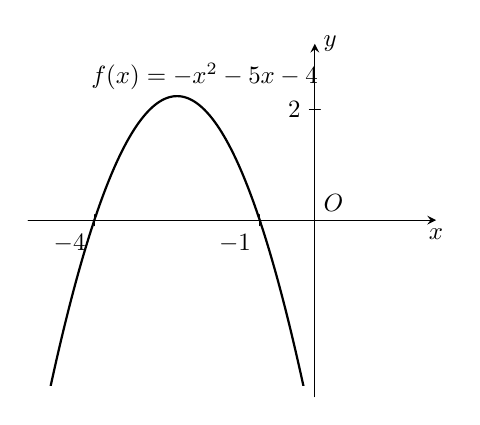
\begin{tikzpicture}[scale=0.7, line join=round, line cap=round, >=stealth]
		\def\xmin{-5}\def\xmax{2}\def\ymin{-3}\def\ymax{3}
		\draw[->] (\xmin-0.2,0)--(\xmax+0.2,0) node[below]{$x$};
		\draw[->] (0,\ymin-0.2)--(0,\ymax+0.2) node[right]{$y$};
		\draw (0,0) node[above right]{$O$};
		\foreach \x in {-4,-1}\draw (\x,0.1)--(\x,-0.1) node[below left]{$\x$};
		\foreach \y in {2}\draw (0.1,\y)--(-0.1,\y) node[left]{$\y$};
		\clip (\xmin,\ymin) rectangle (\xmax,\ymax);
		\draw[thick,smooth,samples=200,domain=\xmin:\xmax] plot (\x,{-1*((\x)^2)+-5*\x+-4});
		\draw (-2,3)node[below]{$f(x)=-x^2-5x-4$};
	\end{tikzpicture}
\end{center}
\loigiai{
Bảng xét dấu của tam thức bậc hai 
\begin{center}

\begin{tikzpicture}[join = round, cap = round, thick, font = \footnotesize, scale = 1]
	\tkzTabInit[lgt=3.5,espcl = 3]
	{$x$ /1, $f(x)$ /1}
	{$-\infty$,$-4$,$-1$,$+\infty$}
	\tkzTabLine{ ,-,z,+,z,-, }
\end{tikzpicture}
\end{center}
Vậy $f(x)>0\Leftrightarrow x\in (-4;-1)$.\\
$f(x)<0\Leftrightarrow x\in (-\infty;-4)\cup (-1;+\infty)$.
}
\end{bt}

% từ: cau-hoi/lop10/0D7_Bat_phuong_trinh_bac_2_mot_an/0D7-1-3_Bai_toan_xet_dau_biet_BXD_do_thi.tex
\begin{bt}%[0D7H1-3]%[ma:d3230bfc]
	Tìm nghiệm và lập bảng xét dấu của tam thức bậc hai $f(x)$ với đồ thị được cho ở mỗi hình\\
	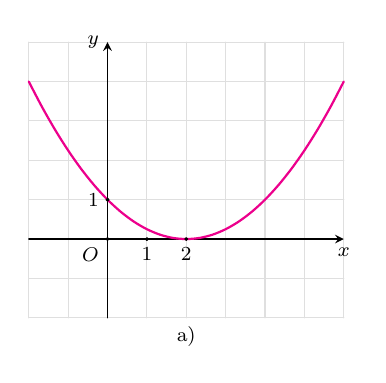
\begin{tikzpicture}[scale=.5, font=\footnotesize, line join=round, line cap=round, >=stealth]
		\draw[gray!50,opacity=.5](-2,-2)grid(6,5);
		\draw[->](-2,0)--(0,0)node[below left]{$O$}--(6,0)node[below]{$x$};
		\draw[->](0,-2)--(0,5)node[left]{$y$};
		\draw[smooth,domain=-2:6,thick,magenta]plot(\x,{1/4*(\x)^2-(\x)+1});
		\draw (2,-2)node[below]{a)};
		\draw(1,0)node[below]{$1$};
		\draw(2,0)node[below]{$2$};
		\draw(0,1)node[left]{$1$};
		\foreach \x in{0,1,2}\draw[fill](\x,0)circle(1pt);
		\draw[fill](0,1)circle(1pt);
		
	\end{tikzpicture}\hspace*{1cm}
	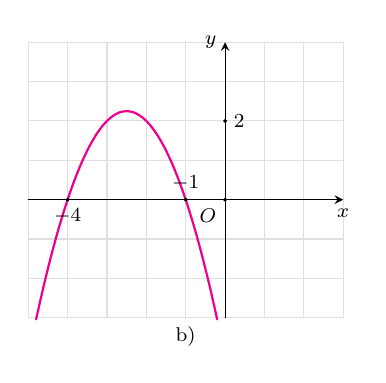
\begin{tikzpicture}[scale=.5, font=\footnotesize, line join=round, line cap=round, >=stealth]
		\draw[gray!50,opacity=.5](-5,-3)grid(3,4);
		\draw[->](-5,0)--(0,0)node[below left]{$O$}--(3,0)node[below]{$x$};
		\draw[->](0,-3)--(0,4)node[left]{$y$};
		\draw[smooth,domain=-4.8:-0.2,thick,magenta]plot(\x,{-(\x)^2-5*(\x)-4});
		\draw (-1,-3)node[below]{b)};
		\draw(-4,0)node[below]{$-4$};
		\draw(0,2)node[right]{$2$};
		\draw(-1,0)node[above]{$-1$};
		\foreach \x in{-4,-1,0}\draw[fill](\x,0)circle(1pt);
		\draw[fill](0,2)circle(1pt);
		
	\end{tikzpicture}\hspace*{1cm}
	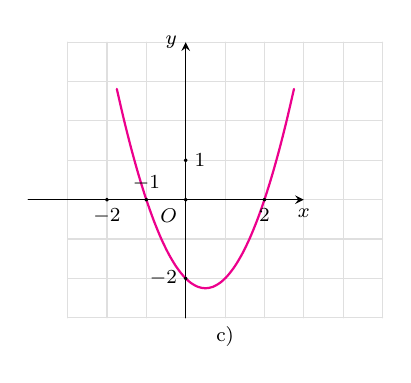
\begin{tikzpicture}[scale=.5, font=\footnotesize, line join=round, line cap=round, >=stealth]
		\draw[gray!50,opacity=.5](-3,-3)grid(5,4);
		\draw[->](-4,0)--(0,0)node[below left]{$O$}--(3,0)node[below]{$x$};
		\draw[->](0,-3)--(0,4)node[left]{$y$};
		\draw[smooth,domain=-1.75:2.75,thick,magenta]plot(\x,{(\x)^2-(\x)-2});
		\draw (1,-3)node[below]{c)};
		\draw(0,1)node[right]{$1$};
		\draw(0,-2)node[left]{$-2$};
		\draw(-2,0)node[below]{$-2$};
		\draw(-1,0)node[above]{$-1$};
		\draw(2,0)node[below]{$2$};
		\foreach \x in {-2,-1,0,2}\draw[fill](\x,0)circle(1pt);
		\foreach \x in {-2,1}\draw[fill](0,\x)circle(1pt);
		
	\end{tikzpicture}
	\loigiai{
		\begin{enumEX}[a)]{1}
			\item \immini{Từ đồ thị hình a) ta có nghiệm của tam thức bậc hai $f(x)$ là $x=2$. Bảng xét dấu của tam thức là}{
				
\begin{tikzpicture}
					\tkzTabInit[deltacl=0.6,espcl=2.5,lgt=2,nocadre=false]
					{$x$/0.6,$f(x)$/0.6}
					{$-\infty$,$2$,$+\infty$}
					\tkzTabLine{,+,0,+,}
					
				\end{tikzpicture}
			}
			\item \immini{Từ đồ thị hình b) ta có tam thức bậc hai $f(x)$ có $2$ nghiệm $x_1=-4$ và $x_2=-1$. Bảng xét dấu của tam thức là}{
				
\begin{tikzpicture}
					\tkzTabInit[deltacl=0.6,espcl=2.5,lgt=2,nocadre=false]
					{$x$/0.6,$f(x)$/0.6}
					{$-\infty$,$-4$,$-1$,$+\infty$}
					\tkzTabLine{,-,0,+,0,-,}
					
				\end{tikzpicture}
			}
			\item \immini{Từ đồ thị hình c) ta có nghiệm của tam thức bậc hai $f(x)$ là $x_1=-1$ và $x_2=2$. Bảng xét dấu của tam thức là}{
				
\begin{tikzpicture}
					\tkzTabInit[deltacl=0.6,espcl=2.5,lgt=2,nocadre=false]
					{$x$/0.6,$f(x)$/0.6}
					{$-\infty$,$-1$,$2$,$+\infty$}
					\tkzTabLine{,+,0,-,0,+,}
					
				\end{tikzpicture}
			}
		\end{enumEX}
	}
\end{bt}

% từ: cau-hoi/lop10/0D7_Bat_phuong_trinh_bac_2_mot_an/0D7-2-3_Bat_phuong_trinh_dang_tich_thuong.tex
\begin{bt}%[0D7T2-3]%[ma:1039bd3d]
	Bác Hùng muốn trồng một vườn hoa trên mảnh đất hình chữ nhật và làm hàng rào bao quanh. Bác Hùng chỉ  mua được $40$ m hàng rào. Gọi $x>0$ (m) là chiều dài hình chữ nhật.
	\begin{enumerate}
		\item Tính diện tích vườn hoa theo $x$ biết rằng bác Hùng  sử dụng hết $40$ m hàng rào.
		\item Bác Hùng muốn diện tích  vườn hoa ít nhất $64$ m$^2$. Hỏi chiều dài của vườn hoa nằm trong khoảng nào?
	\end{enumerate}
	 \loigiai{
		\begin{enumerate}
			\item Chiều rộng của mảnh đất hình chữ nhật là $20-x$ (m).\\ 
			Diện tích của mảnh đất hình chữ nhật  là $x(20-x) = 20x-x^2$ (m$^2$).
			 \item Theo yêu cầu, ta có
			\[20x - x^2 \geq 64 \Leftrightarrow -x^2 + 20x -64\geq 0 \Leftrightarrow 4\leq  x \leq 16.\]
			Mặt khác, ta có  điều kiện $x \geq 20-x \Leftrightarrow x \geq 10$.\\
			Vậy chiều dài $x$ của  vườn hoa thỏa mãn $10\leq x \leq 16$.
		\end{enumerate}
	} 
\end{bt}

% từ: cau-hoi/lop10/0D7_Bat_phuong_trinh_bac_2_mot_an/0D7-2-7_Toan_thuc_te_ung_dung_bat_phuong_trinh_bac_2.tex
\begin{bt}%[0D7H2-7]%[ma:e61cba62]
	Bác Hùng dùng $52$ m lưới thép gai rào  thành một mảnh vườn hình chữ nhật để trồng rau. Hỏi bác Hùng có thể rào được mảnh vườn có diện tích lớn nhất là bao nhiêu mét vuông?
	\shortans{169} 
	\loigiai{ 
		Gọi $x$ (m) là độ dài chiều rộng của mảnh vườn (với $0<x<26$).  \\
		Khi đó  chiều dài là $\dfrac{56-2x}{2}=26-x$ (m).\\
		Diện tích  của hình chữ nhật là $$S=x(26-x)\le\left(\dfrac{x+26-x}{2}\right)^2=169
		\text{  (m}^2)$$
		dấu bằng xảy ra khi $x=26-x\Rightarrow x=13$.\\ 
		Vậy diện tích lớn nhất có  thể rào được mảnh vườn là $169$ m$^2$ với $x=13$ m.
	 }
\end{bt}

% từ: cau-hoi/lop10/0D7_Bat_phuong_trinh_bac_2_mot_an/0D7-2-7_Toan_thuc_te_ung_dung_bat_phuong_trinh_bac_2.tex
\begin{bt}%[0D7V2-7]%[Dự án đề kiểm tra GHKII-NH22-23-TinDatTran]%[ma:1b71f31e]
	Một hình chữ nhật có chu vi bằng $ 40 $ m. Để diện tích hình chữ nhật lớn hơn $ 75 $ m$ ^2 $ thì chiều rộng của hình chữ nhật nằm trong khoảng bao nhiêu?
	\loigiai{
	Gọi $ x $ m là chiều rộng hình chữ nhật. Khi đó chiều dài hình chữ nhật là $ 20-x $ m.\\
	Ta có $ 0<x\leq 20-x \Leftrightarrow 0<x\leq 10 $.\\
	Diện tích hình chữ nhật là $ S=x(20-x) $ m$ ^2 $.\\
	Theo đề bài, ta có $ x(20-x)>75\Leftrightarrow x^2-20x+75<0\Leftrightarrow 5<x<15 $.\\
	So với điều kiện, ta có $ 5<x\leq 10 $.\\
	Vậy chiều rộng của hình chữ nhật nằm trong khoảng từ lớn hơn $5$ đến $10$ m.
	}
\end{bt}

% từ: cau-hoi/lop10/0D7_Bat_phuong_trinh_bac_2_mot_an/0D7-2-7_Toan_thuc_te_ung_dung_bat_phuong_trinh_bac_2.tex
\begin{bt}%[0D7V2-7]%[Dự án đề kiểm tra Toán 10 GHKII NH24-25- Phạm Văn Long]%[THPT Chuyên Lương Thế Vinh-Đồng Nai]%[ma:92dc4778]
	Bạn An muốn trồng một vườn hoa trên một mảnh đất hình chữ nhật và làm hàng rào bao quanh. An chỉ có đủ vật liệu để làm $40$ m hàng rào, nhưng An muốn diện tích vườn hoa ít nhất $84$ m$^2$. Hỏi chiều rộng của mảnh vườn ít nhất bằng bao nhiêu mét?
	\shortans{6}
	\loigiai{
	Gọi $x$ m là chiều rộng của mảnh vườn ($0<x<20$).\\
	Suy ra chiều dài của mảnh vườn là $20-x$ m.\\
	Diện tích vườn hoa là $x\cdot (20-x)$ m$^2$.\\
	Khi đó ta có bất phương trình $$x\cdot (20-x)\ge 84\Leftrightarrow -x^2+20x-84\ge 0\Leftrightarrow 6\le x \le 14.$$
	Vậy chiều rộng của mảnh vườn ít nhất bằng $6$ m.
	}
\end{bt}

% từ: cau-hoi/lop10/0D7_Bat_phuong_trinh_bac_2_mot_an/0D7-3-1_Phuong_trinh_can.tex
\begin{ex}%[0D7V3-1]%[ma:fb9787c5]
	Cho phương trình $(x+1)\left( \sqrt{x+4} - \sqrt{-x^2 + 4x + 14} \right) = 0 \quad (1)$.  Khi đó
	 \choiceTF
		{Phương trình $(1)$  không có nghiệm bé hơn $4$}
		{\True Phương trình $(1)$  có $3$ nghiệm phân biệt}
		{\True Các  nghiệm của phương trình $(1)$ đều là số nguyên}
		{Tổng bình phương các nghiệm của  phương trình $(1)$ bằng $29$}
	\loigiai{ 
		Ta  có
		\[ 
		(1) \Rightarrow \hoac{&x+1 = 0 \\ & \sqrt{x+4} - \sqrt{-x^2 + 4x  + 14} = 0}
		\Rightarrow \hoac{&x=-1\\ &x+4 =  -x^2 + 4x + 14}
		\Leftrightarrow \hoac{&x=-1\\ &x^2 - 3x -  10 = 0.}
		\] 
		Từ đó ta giải được các nghiệm $x=-1$, $x=-2$,  $x=5$.\\
		Thử lại ta  thấy $x=-1$, $x=-2$ và $x=5$ đều thoả mãn. Vậy
		\begin{itemchoice}
			\itemch Phương trình có nghiệm  $x=-1 < 4$.
			\itemch Phương trình $(1)$ có $3$ nghiệm $x=-1$, $x=-2$  và $x=5$.
			\itemch Ta có $-1$; $-2$; $5$ đều  là các số nguyên.
			\itemch Ta có $(-1)^2 + (-2)^2  + 5^2 = 30.$
		\end{itemchoice}
	 }
\end{ex}

% từ: cau-hoi/lop10/0D7_Bat_phuong_trinh_bac_2_mot_an/0D7-3-6_Toan_hinh_toan_thuc_te_ung_dung_phuong_trinh.tex
\begin{bt}%[0D7V3-6]%[ma:4bf8a111]
	Người ta muốn thiết kế một vườn hoa hình chữ nhật nội tiếp trong một miếng đất hình tròn có đường kính bằng $50$\,m.  Tính diện tích vườn hoa hình chữ nhật (đơn vị: m$^2$), biết tổng quãng đường đi xung quanh vườn hoa đó là $140$\,m.
	 \shortans
	{  $1200$}
	\loigiai{ 
	\immini{ 
		Gọi chiều rộng  hình chữ nhật là $x=AB$\,(m).\\
		Suy ra, chiều dài  hình chữ nhật là
		$BC=\sqrt{AC^2-AB^2}=\sqrt{2500-x^2}$\,(m).\\ 
		Ta có $2\left(x+\sqrt{2500-x^2}\right)=140\Leftrightarrow \sqrt{2500-x^2}=70-x$.\\ 
		Bình phương hai  vế phương trình ta được:
		 \allowdisplaybreaks
		\begin{eqnarray*}
			&&2500-x^2=(70-x)^2 
			 \Leftrightarrow 2500-x^2=4900-140x+x^2
			 \\
			&\Leftrightarrow& 2x^2-140x+2400=0 
			 \Leftrightarrow \hoac{&x=40\\&x=30.}
		\end{eqnarray*}
		} 
		 {
		\begin{tikzpicture}[declare function={r=1.5;},font=\footnotesize,line join=round,line cap=round,>=stealth]
				\path (0:0)  coordinate (O)
					 (30:r) coordinate (A)
					(-30:r) coordinate  (B)
					($(O)!-1!(A)$) coordinate (C) 
					($(O)!-1!(B)$)  coordinate (D);
				\draw (A)--(B)--(C)--(D)--cycle (A)--(C) 
					(O)  circle (r);
				 \foreach \t/\g in {A/0,B/0,C/180,D/180}{
					\draw[fill=black] (\t) circle (1pt)  node[shift={(\g:7pt)},font=\scriptsize]{$ \t $};
				 }
			\end{tikzpicture}
		 }
		\noindent 
		Thử lại, ta thấy $x=40$ và $x=30$ đều thỏa phương  trình.\\
		Vậy phương trình có hai nghiệm là  $\hoac{&x=40\\&x=30.}$\\
		Nếu $x=AB=30\Rightarrow BC=40$.\\ 
		 Nếu $x=AB=40\Rightarrow BC=30$ (loại vì $BC>AB$).\\
		Vậy diện  tích vườn hoa là $40\cdot 30=1\,200\,\mathrm{m}^2$.
	} 
\end{bt}

% từ: cau-hoi/lop10/0D7_Bat_phuong_trinh_bac_2_mot_an/0D7-3-6_Toan_hinh_toan_thuc_te_ung_dung_phuong_trinh.tex
\begin{bt}%[0D7V3-6]%[ma:0dbe7e07]
	Lúc $8$ giờ sáng, hai ô tô cùng xuất phát tại vị trí $A$ và vị trí $B$ cách nhau $100$ km chạy về thành phố $T$. Vận tốc của hai ô tô chạy từ vị trí $A$ và vị trí $B$ lần lượt là $55$ km/h và $45$ km/h. Biết rằng tại thời điểm ô tô đi từ vị trí $A$ đến địa điểm $D$ cách thành phố $T$ $14$ km thì  ô tô đi từ vị trí $B$ đến địa điểm $C$ cách thành phố $T$ là $6$ km. Hỏi thời điểm đó là mấy giờ? (Đơn vị tính $24$ h).
	\begin{center}
		\begin{tikzpicture}
				 \def\r{5}
				\path (0:0) coordinate  (A)
					++(0:\r)  coordinate (T)
					++(-90:0.7*\r) coordinate  (B)
					 (A)++(0:0.5*\r) coordinate (D)
					(T)++(-90:0.2*\r) coordinate (C); 
				 \draw (A)--(D)
					(D)--(T) node [midway,above] {$14$ km} 
					(T)--(C)  node [midway,right] {$6$ km}
					(C)--(B) 
					pic[draw,angle radius=2mm]{right  angle=A--T--B}
					(B)--(A) node [midway,below  left] {$100$ km};
				\foreach  \x/ \goc in {A/135,B/-45,T/45,D/90,C/0}
				\fill (\x) circle  (1pt)
					($(\x)+(\goc:3mm)$)  node {$\x$};
			\end{tikzpicture}
	\end{center}
	\loigiai{ 
		Gọi $x$ (giờ) là thời gian ô tô đi từ vị trí $A$ đến địa điểm $D$ $(x  > 0)$.\\
		Vì hai ô tô xuất phát cùng một lúc nên thời gian ô tô đi từ vị trí $B$ đến  địa điểm $C$ cũng là $x$ giờ. Do đó, quảng đường $AD$ và $BC$ lần lượt là $55x$ km và $45x$ km.\\
		Suy ra khoảng cách từ  vị trí $A$ và vị trí $B$ đến thành phố $T$ lần lượt là $55x+14$ km và $45x+6$ km.
		Vì khoảng cách giữa hai vị trí $A$ và $B$ là $100$  km nên ta có phương trình
		 \[\sqrt{(55x+14)^2+(45x+6)^2}=100\Leftrightarrow 5\,050x^2+2\,080x+232=10\,000.\]
		Giải phương trình này và kết hợp với điều kiện $x  > 0$, ta nhận $x=\dfrac{6}{5}$.\\
		Đổi $\dfrac{6}{5}$ giờ $=1$ giờ $12$  phút.\\
		Vậy thời điểm ô tô đi từ vị trí  $A$ đến địa điểm $D$ là $8$ giờ $+$ $1$ giờ $12$ phút $=$ $9$ giờ $12$ phút.
	} 
\end{bt}

% từ: cau-hoi/lop10/0D7_Bat_phuong_trinh_bac_2_mot_an/0D7-3-6_Toan_hinh_toan_thuc_te_ung_dung_phuong_trinh.tex
\begin{bt}%[0D7V3-6]%[ma:b5503141]
	Hằng  ngày bạn Hùng đều đón bạn Minh đi học tại một vị trí trên lề đường thẳng đến trường. Minh đứng tại vị trí $A$ cách lề đường một khoảng $50$ (m) để chờ Hùng. Khi nhìn thấy Hùng đạp xe đến địa điểm $B$, cách mình một đoạn $200$ (m) thì Minh bắt đầu đi bộ ra lề đường đến điểm $C$ để bắt kịp xe. Vận tốc đi bộ Minh là $5$ (km/h), vận tốc xe đạp của Hùng là $15$ (km/h). Vị trí $C$ trên lề đường cách điểm $B$ bao nhiêu mét để hai bạn gặp nhau mà không bạn nào phải chờ người kia.
	\begin{center}
		\begin{tikzpicture}[line cap=round,line join=round,font=\footnotesize,>=stealth,scale=1]
				\tikzset{label style/.style={font=\footnotesize}} 
				\path (0,0)  coordinate (H)
					(0,-2) coordinate  (A)
					(-7.746,0) coordinate  (B)
					(-1.849,0) coordinate (C); 
				\draw (A)--(H)  node[midway,right]{$50$ m}--(B)--(A) node[midway,sloped,below]{$200$ m}--(C) node[above,pos=0.3,sloped]{\tikz \draw[<-,thick] (0,0)--(1,0);};
				\foreach\x/\y in {A/-45,B/-90,C/90,H/90} \draw[fill=black]  (\x) circle (1pt)+(\y:0.3) node{$\x$};
				 \draw (B) node[above]{Hùng}
					($(B)+(1,0)$) node[above]{\tikz \draw[->,thick]  (0,0)--(1,0);}
					(A)  node[below left]{Minh};
				\draw  pic[draw,angle radius=2mm]{right angle=A--H--B};
			\end{tikzpicture}
	\end{center}
	\loigiai{ 
		Tam  giác vuông $AHB$ có $BH=\sqrt{(0{,}2)^2-(0{,}05)^2}=\dfrac{\sqrt{15}}{20}$ (km).\\
		 Gọi $BC=x$ (km) $x>0$.\\
		Suy  ra $CH=\dfrac{\sqrt{15}}{20}-x$, $x\le\dfrac{\sqrt{15}}{20}$.\\
		Ta cần xác định vị trí điểm $C$ để Minh và Hùng gặp nhau mà không  bạn nào phải chờ người kia.\\
		Nghĩa là: ta cần tìm $x$ để thời gian  hai bạn di chuyển đến $C$ là bằng nhau.
		Thời gian Hùng đi từ $B$  đến $C$ là $t_2=\dfrac{S_{BC}}{15}=\dfrac{x}{15}$ (h).\\
		Quảng đường $AC$ Minh đã đi là $AC=\sqrt{CH^2+AH^2}=\sqrt{\left(\dfrac{\sqrt{15}}{20}-x\right)^2+(0{,}05)^2}$.\\ 
		Thời gian Minh đã đi từ  $A$ đến $C$ là $t_1=\dfrac{S_{AC}}{5}=\dfrac{\sqrt{\left(\dfrac{\sqrt{15}}{20}-x\right)^2+(0{,}05)^2}}{5}$ (h).\\
		Theo yêu cầu bài toán ta có $\dfrac{\sqrt{\left(\dfrac{\sqrt{15}}{20}-x\right)^2+(0{,}05)^2}}{5}=\dfrac{x}{15}$.\\ 
		Bình phương hai vế  ta được
		\begin{align*}
			\dfrac{\left(\dfrac{\sqrt{15}}{20}-x\right)^2+(0{,}05)^2}{25}=\dfrac{x^2}{225} 
			&\Leftrightarrow  9\left(\dfrac{3}{80}-\dfrac{\sqrt{15}}{10}x+x^2\right)+\dfrac{9}{400}=x^2\\
			&\Leftrightarrow 8x^2-\dfrac{9\sqrt{15}}{10}x+\dfrac{9}{25}=0\Leftrightarrow \hoac{&x\approx  0{,}3\\&x\approx0{,}1.}
		\end{align*}
		Vì $0<x\le\dfrac{\sqrt{15}}{20}\approx  0{,}19$ nên $x\approx 0{,}168$, thỏa mãn.\\
		Vậy hai bạn Minh và Hùng di chuyển đến vị trí $C$ cách điểm $B$  một đoạn $x\approx 0{,}168$ (km) $=168$ (m).
	} 
\end{bt}

% từ: cau-hoi/lop10/0D7_Bat_phuong_trinh_bac_2_mot_an/0D7-3-6_Toan_hinh_toan_thuc_te_ung_dung_phuong_trinh.tex
\begin{bt}%[0D7V3-6]%[ma:5eacd623]
	Hằng ngày bạn Hùng đều đón bạn Minh đi học tại một vị trí trên lề đường thẳng đến trường. Minh đứng tại vị trí $A$ cách lề đường một khoảng $50$ m  để chờ Hùng. Khi nhìn thấy Hùng đạp xe đến địa điểm $B$, cách mình một đoạn $200$ m thì Minh bắt đầu đi bộ ra lề đường để bắt kịp xe. Vận tốc đi bộ của Minh là $5$ km/h, vận tốc xe đạp của Hùng là $15$ km/h. Hãy xác định vị trí $C$ trên lề đường để hai bạn gặp nhau mà không bạn nào phải chờ người kia. (làm tròn kết quả đến hàng phần muời)
	\begin{center}
		\begin{tikzpicture}[thick,scale=1.5]
				\path (0,0)  coordinate (B) node[above]{Hùng}
					(6,0) coordinate  (C)++(-35:2.5) coordinate (A) node[below left]{Minh}
					 ($(B)!(A)!(C)$) coordinate (H);
				\draw  (B)--(A)--(H)
					 (A)--(C)
					($(B)!-.1!(H)$)--($(H)!-.1!(B)$); 
				 \foreach \x/\g in {A/0,B/-90,C/90,H/90}
				\fill[black]  (\x) circle (1pt)
					 ($(\g:3mm)+(\x)$) node {$\x$};
				\path (A)--(B) node[pos=.45,below left]{$200$  m}
					(A)--(H) node[pos=.5,right]{$50$ m}; 
				 \draw pic[draw,angle radius=2mm]{right angle=B--H--A};
				 \draw[-stealth] (B)++(30:.5)--++(0:1);
				 \draw[-stealth] (A)++(120:.3)--++(145:.6);
			\end{tikzpicture}
	\end{center}
	 \loigiai{
		Vận tốc của bạn Minh:  $v_{1}=5$ km/h,
		 vận tốc của bạn Hùng: $v_{2}=15$ km/h. \\
		Áp  dụng định lý Pythagore vào tam giác vuông $AHB$, ta có
		\allowdisplaybreaks 
		\begin{eqnarray*}
			 BH=\sqrt{(0{,}2)^{2}-(0{,}05)^{2}}=\dfrac{\sqrt{15}}{20} \text{ km}.
		\end{eqnarray*}
		Gọi $B C=x$ (km),  $x>0$.\\
		Suy ra $C  H=\dfrac{\sqrt{15}}{20}-x$, $x \leq \dfrac{\sqrt{15}}{20}$. \\
		Ta cần xác định vị trí điểm $C$ để Minh và Hùng gặp nhau mà không bạn nào phải chờ người kia nghĩa  là ta cần tìm $x$ để thời gian hai bạn di chuyển đến $C$ là bằng nhau. \\
		Thời gian Hùng đi từ $B$ đến $C$  là $t_{2}=\dfrac{S_{B C}}{v_{2}}=\dfrac{x}{15}$ (h). \\
		Quãng đường $A C$ Minh đã đi  là $A C=\sqrt{C H^{2}+A H^{2}}=\sqrt{\left(\dfrac{\sqrt{15}}{20}-x\right)^{2}+(0{,}05)^{2}}$ \\
		Thời gian Minh đã đi từ $A$ đến $C$ là $t_{1}=\dfrac{S_{A C}}{v_{1}}=\dfrac{\sqrt{\left(\dfrac{\sqrt{15}}{20}-x\right)^{2}+(0{,}05)^{2}}}{5}$ (h).  \\
		Theo yêu cầu bài  toán $\dfrac{\sqrt{\left(\dfrac{\sqrt{15}}{20}-x\right)^{2}+(0{,}05)^{2}}}{5}=\dfrac{x}{15}$. \\
		Bình phương 2 vế: 
		 \allowdisplaybreaks
		\begin{eqnarray*}
			&&\dfrac{\left(\dfrac{\sqrt{15}}{20}-x\right)^2+(0{,}05)^2}{25}=\dfrac{x^2}{225}\\ 
			&\Leftrightarrow& 9\left(\dfrac{3}{80}-\dfrac{\sqrt{15}}{10} x+x^2\right)+\dfrac{9}{400}=x^2 \\ 
			 &\Leftrightarrow& 8x^2-\dfrac{9\sqrt{15}}{10} x+\dfrac{9}{25}=0\\
			&\Leftrightarrow& 
			\hoac{&x \approx 0{,}3\\ 
			&x \approx 0{,}1.} 
		\end{eqnarray*}
		Vì $0<x \leq \dfrac{\sqrt{15}}{20} \approx 0{,}19$ nên $x  \approx 0{,}1$ thỏa mãn. \\
		Vậy hai bạn  Minh và Hùng di chuyển đến vị trí $C$ cách $B$ một đoạn $x \approx 0{,}1$ km $=100$ m.
	 }
\end{bt}

% từ: cau-hoi/lop10/0D7_Bat_phuong_trinh_bac_2_mot_an/0D7-3-6_Toan_hinh_toan_thuc_te_ung_dung_phuong_trinh.tex
\begin{bt}%[Dự án Bài Giảng 10-11 Nhóm Toán & LaTex, Nguyễn Anh Tuấn]%[0D7V3-6]%[ma:72f6f066]
	\immini{
		Từ một tấm tôn có hình dạng là nửa hình tròn bán kính $R=3$, người ta muốn cắt ra một hình chữ nhật (hình vẽ bên). Tính độ dài cạnh $MQ$, biết chu vi hình chữ nhật bằng $12$.
	}
	{
		\begin{tikzpicture}[thick,scale=0.7]
			\draw [-] (-4,0)--(4,0);
			\draw [-] (-3,0)--(-2.99,2.65)--(2.99,2.65)--(3,0);
			\draw[smooth,samples=200,variable=\t,domain=0:180] plot({(4)*cos (\t)},{(4)*sin(\t)});
			\draw (0,0) [fill=black] circle (1pt) node[below]{$O$};
			\draw (-3,0) [fill=black] circle (1pt) node[below]{$Q$};
			\draw (3,0) [fill=black] circle (1pt) node[below]{$P$};
			\draw (-2.99,2.65) [fill=black] circle (1pt) node[left]{$M$};
			\draw (2.99,2.65) [fill=black] circle (1pt) node[right]{$N$};
			\draw[pattern=north east lines,pattern color=black!50!] (-3,0)--(-2.99,2.65)--(2.99,2.65)--(3,0);
		\end{tikzpicture}
	}
	\loigiai{
		Đặt $OQ=x,\ (0<x<3) \Rightarrow MQ=\sqrt{MO^2-OQ^2}=\sqrt{9-x^2}$.\\
		Ta có  $4x+2\sqrt{9-x^2}=12\Leftrightarrow \sqrt{9-x^2}=6-2x\Leftrightarrow 5x^2-24x+27=0\Leftrightarrow\hoac{&x=3\text{ (loại)}\\&x=1{,}8.}$\\
		Vậy $MQ=\dfrac{12}{5}$.
	}
\end{bt}

% từ: cau-hoi/lop10/0D7_Bat_phuong_trinh_bac_2_mot_an/0D7-3-6_Toan_hinh_toan_thuc_te_ung_dung_phuong_trinh.tex
\begin{bt}%[0D7V3-6]%[ma:ed9edc54]
	Để leo lên một bức tường, bác Nam dùng một chiếc thang có chiều dài cao hơn bức tường đó $1$ m. Ban đầu, bác Nam đặt chiếc thang mà đầu trên của chiếc thang đó vừa chạm vào mép trên bức tường (Hình a). Sau đó, bác Nam dịch chuyển chân thang vào gần chân tường thêm $0{,}5$ m thì bác Nam nhận thấy thang tạo với mặt đất một góc $60^\circ$ (Hình b). Bức tường cao bao nhiêu mét (làm tròn kết quả đến hàng phần mười)?
	\begin{center}
		\begin{tikzpicture}[scale=0.8, line join=round, line cap=round,>=stealth]
			\path
			(-1,0) coordinate (P)+(-80:1) node{Hình a)}
			(P)+(60:5) coordinate (Q)
			(P)+(-30:0.2) coordinate (P1)+(-90:.3) node{$B$}
			(Q)+(-30:0.2) coordinate (Q1)+(0:.3) node{$A$}
			(P)+(150:0.9) coordinate (PP)
			(Q)+(150:0.9) coordinate (QQ)
			(P1)+(150:0.9) coordinate (PP1)
			(Q1)+(150:0.9) coordinate (QQ1)
			(4,0) coordinate (SD)
			(SD)+(150:10) coordinate (ST)
			(Q1)+(-90:1) coordinate (QT)
			(Q)+(0:1) coordinate (Q2)
			(intersection of SD--ST and Q1--QT) coordinate (C)+(-90:.3) node{$C$}
			;
			\draw (-2,-0.5) rectangle (2,5.5);
			\clip (-2,-0.5) rectangle (2,5.5);
			\foreach \b in {0.1,0.2,...,0.9} {
				\path 
				($(P)!\b!(Q)$) coordinate (m)
				(m)+(50:0.2)coordinate (m1)
				(m)+(150:0.7)coordinate (m2)
				(m1)+(150:0.7)coordinate (m3);
				\draw[fill=cyan!50](m)--(m1)--(m3)--(m2)--(m);}
			\draw[fill=cyan!50] (P)--(Q)--(Q1)--(P1)--(P);
			\draw[fill=cyan!50] (PP)--(QQ)--(QQ1)--(PP1)--(PP);
			\draw (SD)--(ST) (P1)--(C)--(Q1);
			\draw (Q1)--++(-30:2) (Q1)--++(150:3);
			\draw (Q2)--++(-30:2) (Q2)--++(150:3);
			\pic[draw,angle radius=10]{right angle=P1--C--Q1};
		\end{tikzpicture}
		\begin{tikzpicture}[scale=0.8, line join=round, line cap=round,>=stealth]
			\path
			(-1,0) coordinate (P)+(-80:1) node{Hình b)}
			(P)+(70:5) coordinate (Q)
			(P)+(-30:0.2) coordinate (P1)+(-90:.3) node{$E$}
			(Q)+(-30:0.2) coordinate (Q1)
			(P)+(150:0.9) coordinate (PP)
			(Q)+(150:0.9) coordinate (QQ)
			(P1)+(150:0.9) coordinate (PP1)
			(Q1)+(150:0.9) coordinate (QQ1)
			($(P1)!0.9!(Q1)$) coordinate (D)+(0:.3) node{$D$}
			(4,-1) coordinate (SD)
			(SD)+(150:10) coordinate (ST)
			(D)+(-90:1) coordinate (QT)
			(D)+(0:1) coordinate (Q2)
			(intersection of SD--ST and Q1--QT) coordinate (C)+(0:.3) node{$G$}
			;
			\draw (-2,-0.5) rectangle (1.7,5.5);
			\clip (-2,-0.5) rectangle (1.7,5.5);
			\foreach \b in {0.1,0.2,...,0.9} {
				\path 
				($(P)!\b!(Q)$) coordinate (m)
				(m)+(70:0.2)coordinate (m1)
				(m)+(150:0.7)coordinate (m2)
				(m1)+(150:0.7)coordinate (m3);
				\draw[fill=cyan!50](m)--(m1)--(m3)--(m2)--(m);}
			\draw[fill=cyan!50] (P)--(Q)--(Q1)--(P1)--(P);
			\draw[fill=cyan!50] (PP)--(QQ)--(QQ1)--(PP1)--(PP);
			\draw (SD)--(ST) (P1)--(C)--(D);
			\draw (D)--++(-30:2) (D)--++(150:3);
			\draw (Q2)--++(-30:2) (Q2)--++(150:3);
			\pic[draw,angle radius=10]{right angle=P1--C--Q1};
			\begin{scope}
				\clip (D)--(P1)--(C);
				\draw[fill=yellow] (P1) circle(.6);
			\end{scope}
		\end{tikzpicture}
	\end{center}
	\loigiai{
		Gọi chiều cao bức tường là $x$ ($x>0$). Chiều dài của thang là $x+1$.\\
		Với Hình a, ta có 
		\[BC=\sqrt{AB^2-AC^2}=\sqrt{(x+1)^2-x^2}=\sqrt{2x+1}.\]
		Với Hình b, ta có $EG=BC-0{,}5=\sqrt{2x+1}-0{,}5$, $DG=x$ và $\widehat{DEG}=60^\circ$. Do đó
		\[DG=EG\cdot \tan 60^\circ\Leftrightarrow x=\left(\sqrt{2x+1}-0{,}5\right)\sqrt{3}\Leftrightarrow \sqrt{6x+3}=x+\dfrac{\sqrt{3}}{2}.\qquad (*)\]
		Bình phương hai vế phương trình $(*)$ ta được
		\allowdisplaybreaks 
		\begin{eqnarray*}
			&&6x+3=\left(x+\dfrac{\sqrt{3}}{2}\right)^2 \\
			&\Leftrightarrow& x^2+\left(\sqrt{3}-6\right)x-\dfrac{9}{4}=0\\
			&\Leftrightarrow& \hoac{&x\approx 4{,}7\\&x\approx-0{,}5.}
		\end{eqnarray*}
		Vậy, bức tường cao xấp xỉ $4{,}7$ m.
	}	
\end{bt}

% từ: cau-hoi/lop10/0D7_Bat_phuong_trinh_bac_2_mot_an/0D7-3-6_Toan_hinh_toan_thuc_te_ung_dung_phuong_trinh.tex
\begin{bt}%[0D7V3-6]%[Tex hoa sach Toan 10]%[Đỗ Đường Hiếu]%[ma:a52ed0eb]
	\immini{Một ngọn hải đăng đặt tại vị trí $A$ cách bờ biển một khoảng cách $AB=4$ km. Trên bờ biển có một cái kho ở vị trí $C$ cách $B$ một khoảng là $7$ km. Người canh hải đăng có thể chèo thuyền từ $A$ đến vị trí $M$ trên bờ biển với vận tốc $3$ km/h rồi đi bộ đến $C$ với vận tốc $5$ km/h như hình bên. Tính khoảng cách từ vị trí $B$ đến $M$, biết thời gian người đó đi từ $A$ đến $C$ là $148$ phút.}
	{\begin{tikzpicture}[scale=0.8, line join=round, line cap=round,>=stealth]
			\def\h{1}\def\a{3}\def\b{6}
			\path
			(0:0) coordinate (B)
			(90:\a) coordinate (A)
			(0:\b) coordinate (C)
			($(C)!0.7!(B)$) coordinate (M)
			;
			% sông
			\draw (A)--(B)node[midway,sloped,below]{$4$ km}--(C)
			(A)--(M)
			(B)--++(180:\h) (C)--++(0:\h)
			;
			\draw[dashed] (B)--++(-90:\h) (C)--++(-90:\h);
			\draw[<->] ([yshift=-5mm]B)--([yshift=-5mm]C)node[midway,sloped,below]{$7$ km};
			\foreach \p/\q in{A/90,B/150,C/90,M/50}\fill(\p)circle(1pt)+(\q:.5)node{$\p$};
	\end{tikzpicture}}
	\loigiai{
		Đặt $BM=x$ km ($0<x<7$), khi đó $CM=7-x$ và $AM=\sqrt{16+x^2}$.\\
		Ta có 
		\allowdisplaybreaks 
		\begin{eqnarray*}
			&&\dfrac{AM}{3}+\dfrac{MC}{5}=\dfrac{148}{60}\\
			&\Leftrightarrow&\dfrac{\sqrt{16+x^2}}{3}+\dfrac{7-x}{5}=\dfrac{37}{15}\\
			&\Leftrightarrow& 5\sqrt{16+x^2}=3x+16\\
			&\Leftrightarrow& 25(16+x^2)=(3x+16)^2\\
			&\Leftrightarrow& 16x^2-96x+144=0\\
			&\Leftrightarrow& x^2-6x+9=0\\
			&\Leftrightarrow& x=3.
		\end{eqnarray*}
		Vậy $BM=3$ km.
	}	
\end{bt}

% từ: cau-hoi/lop10/0D7_Bat_phuong_trinh_bac_2_mot_an/0D7-3-6_Toan_hinh_toan_thuc_te_ung_dung_phuong_trinh.tex
\begin{bt}%[0D7V3-6]%[0D6KH-2]%[ma:67c68486]
	Người thứ nhất chèo thuyền với vận tốc $6$ (km/h) vào bờ biển từ một ngọn hải đăng đặt tại vị trí $A$ cách bờ biển một khoảng $AB=4$ (km). Trên bờ biển, người thứ hai đi xe máy với vận tốc $10$ (km/h) từ một nhà kho ở vị trí $C$ cách $B$ một khoảng $BC=7$ (km) (hình vẽ bên dưới). Xác định vị trí hai người gặp nhau ở vị trí $M$ đến $C$, biết hai người xuất phát cùng một lúc.
	\begin{center}
		\begin{tikzpicture}[line join=round,line cap=round,line width=.6pt,font=\footnotesize,scale=1]
			\coordinate[label=above left:$A$](A) at (0,3);
			\coordinate[label=above left:$B$](B) at (0,0);
			\coordinate[label=above right:$C$](C) at (6,0);
			\coordinate(D) at (7,0);
			\coordinate(E) at (-1,0);
			\coordinate[label=above right:$M$] (M) at ($(B)!0.5!(C)$);
			\tkzDrawPoints[fill=black,size=3](A,B,C,M)
			\draw (D)--(E) (A)--(B) (A)--(M);
			\draw[very thick] (M)--(C);
			\coordinate[label=above:$x$] (X) at ($(M)!0.5!(C)$);
			\draw[<->] (0,-0.5)--(6,-0.5) node[midway, fill=white] {$7\,\,km$};
		\end{tikzpicture}
	\end{center}
	\loigiai{
		Đặt $MC=x$ km điều kiện $0<x<7$.\\
		Quãng đường $AM=\sqrt{AB^2+BM^2}$ =$\sqrt{16+( 7-x )^2}$.\\
		Suy ra thời gian đi quãng đường $AM$ là $\dfrac{\sqrt{16+( 7-x )^2}}{6}$ giờ.\\
		Quãng đường $MC=x$ suy ra thời gian đi quãng đường $MC$ là $\dfrac{x}{10}$ giờ.\\
		Giải phương trình $\dfrac{\sqrt{16+( 7-x )^2}}{6}=\dfrac{x}{10}$, ta sẽ được vị trí $M$ đến $C$.\\
		Ta có 
		\begin{eqnarray*}
			\dfrac{\sqrt{16+( 7-x )^2}}{6}=\dfrac{x}{10} &\Leftrightarrow &5\sqrt{16+( 7-x )^2}=3x\\
			&\Rightarrow &25(16+(7-x)^2)=9x^2 \Rightarrow  25x^2 -350x+1625=9x^2\\
			&\Rightarrow & 16x^2-350x+1625=0 \Rightarrow \hoac{
				&x\approx 6{,}687\,\, (\text{nhận})\\
				&x\approx 15{,}188. \,\, (\text{loại})
			}
		\end{eqnarray*}
		Vậy hai nguời gặp nhau ở vị trí $M$ cách $C$ một khoảng cách $6{,}687$ km.
	}
\end{bt}

% từ: cau-hoi/lop10/0D7_Bat_phuong_trinh_bac_2_mot_an/0D7-3-6_Toan_hinh_toan_thuc_te_ung_dung_phuong_trinh.tex
\begin{bt}%[0D7V3-6]%[Dự án đề kiểm tra GKII NH22-23 - Thành Đức Trung]%[THPT Trần Phú - Hồ Chí Minh]%[ma:d1852ed5]
\immini
{
Một người chạy bộ từ vị trí $A$ đến vị trí $C$ trên đoạn đường $BD$, sau đó đạp xe từ vị trí $C$ đến vị trí $B$. Biết rằng vận tốc chạy bộ là $6$km/h, vận tốc đạp xe là $8$km/h, khoảng cách từ vị trí $A$ đến đoạn đường $BD$ bằng $3$km, khoảng cách giữa hai vị trí $B$ và $D$ bằng $8$km. Tính khoảng cách lớn nhất giữa hai vị trí $B$, $C$ biết rằng tổng thời gian người đó chạy bộ và đạp xe là $1$ giờ $20$ phút.
}
{
\begin{tikzpicture}[scale=1, font=\footnotesize, line join=round, line cap=round, >=stealth]
\path
(0,0)coordinate(D)
(8,0)coordinate(B)
(20/7,0)coordinate(C)
(0,3)coordinate(A)
($(A)!0.5!(D)$)node[left]{$3$km}
($(B)!0.5!(D)-(0,0.5)$)node[below]{$8$km}
;
\draw(A)--(D)--(B)--(A)--(C);
\draw[<->, dashed]($(D)-(0,0.5)$)--($(B)-(0,0.5)$);
\foreach \p/\q in {A/90, D/-90, B/-90, C/-90} \fill[black] (\p) circle (2pt) ($(\p)+(\q:2.5mm)$) node{$\p$};
\end{tikzpicture}
}
\loigiai
{\\
Đặt $CD=x$ ($0\leqslant x\leqslant8$; đơn vị km), suy ra $BC=8-x$ (km). \\
Ta có $AC=\sqrt{AD^2+CD^2}=\sqrt{x^2+9}$ (km). \\
Thời gian chạy bộ là $\dfrac{\sqrt{x^2+9}}{6}$ (giờ). \\
Ta có $1$ giờ $20$ phút bằng $\dfrac{4}{3}$ giờ. \\
Suy ra thời gian đạp xe là $\dfrac{4}{3}-\dfrac{\sqrt{x^2+9}}{6}=\dfrac{8-\sqrt{x^2+9}}{6}$ (giờ). \\
Do đó $BC=8\cdot\dfrac{8-\sqrt{x^2+9}}{6}=\dfrac{32-4\sqrt{x^2+9}}{3}$ (km). \\
Ta có phương trình $8-x=\dfrac{32-4\sqrt{x^2+9}}{3} \Leftrightarrow 4\sqrt{x^2+9}=3x+8$. \hfill $(1)$ \\
Bình phương hai vế phương trình $(1)$ ta có $16\left(x^2+9\right)=\left(3x+8\right)^2 \Leftrightarrow 7x^2-48x+80=0 \Leftrightarrow \hoac{ & x=4 \\ & x=\dfrac{20}{7}.}$ \\
Thay thử lại vào phương trình $(1)$ ta thấy hai nghiệm $x=4$, $x=\dfrac{20}{7}$ thỏa mãn. \\
Với $x=4$ ta có $BC=4$ (km). \\
Với $x=\dfrac{20}{7}$ ta có $BC=\dfrac{36}{7}$ (km). \\
Vậy khoảng cách lớn nhất giữa hai vị trí $B$, $C$ là $\dfrac{36}{7}$km. \\
}
\end{bt}

% từ: cau-hoi/lop10/0D7_Bat_phuong_trinh_bac_2_mot_an/0D7-3-6_Toan_hinh_toan_thuc_te_ung_dung_phuong_trinh.tex
\begin{bt}%[0D7H3-6]%[Tex hóa SGK CD-CT,T7/22, Tuấn Nguyễn]%[ma:40856b8d]
	\immini
	{Một người đứng ở điểm $A$ trên một bờ sông rộng $300$ m, chèo thuyền đến vị trí $D$, sau đó chạy bộ đến vị trí $B$ cách C một khoảng $800$ m như Hình 34. Vận tốc chèo thuyền là $6$ km/h, vận tốc chạy bộ là $10$ km/h và giả sử vận tốc dòng nưốc không đáng kể. Tính khoảng cách từ vị trí $C$ đến $D$, biết tổng thời gian người đó chèo thuyền và chạy bộ từ $A$ đến $B$ là $7{,}2$ phút.}
	{
		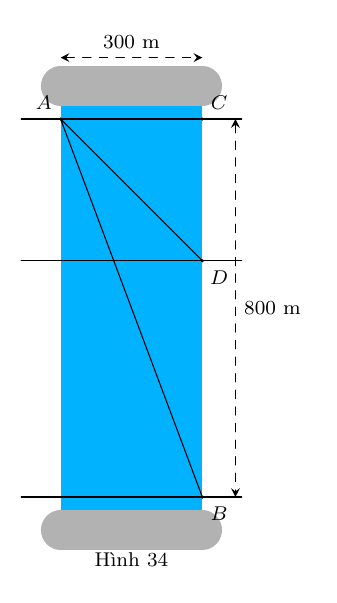
\begin{tikzpicture}[scale=0.6, font=\footnotesize, line join=round, line cap=round, >=stealth]
			\fill[blue!30!cyan] (0,-8.5) rectangle (3,0.5);
			\path 
			(0,0) coordinate (A)
			(3,0) coordinate (C)
			(3,-3) coordinate (D)
			(3,-8) coordinate (B)
			(1.5,-9) coordinate (FF) node[below]{Hình 34}
			;
			\foreach  \x in {0,-3,-8}{
				\draw[shorten <= -0.5cm,shorten >= -0.5cm,shift={(0,\x)}] (0,0)--(3,0);
			}	
			\foreach  \x in {0.7,-8.7}{
				\draw[shift={(0,\x)},line width=0.5cm,black!30] (0,0)--(3,0);
			}	
			\draw[<->,dashed] (0,1.3)--(3,1.3) node[above,midway]{$300$ m};
			\draw (B)--(A)--(D);
			\draw[<->,dashed] (3.7,0)--(3.7,-8) node[right,midway]{$800$ m};
			\foreach \p/\g in {A/135,B/-45,C/45,D/-45}\fill[black] (\p) circle (1pt) +(\g:.5)node{$\p$};
	\end{tikzpicture}}
	\loigiai{
		Gọi $CD=a$ km suy ra $BD=0{,}8-a$ km ($0<a< 0{,}8$).\\
		Theo giả thiết ta có $AD=\sqrt{AC^2+CD^2}=\sqrt{0{,}3^2+a^2}$.\\
		Từ đó suy ra \begin{eqnarray*}
			&&\dfrac{\sqrt{0{,}3^2+a^2}}{6}+\dfrac{0{,}8-a}{10}=\dfrac{7{,}2}{60}\\
			&\Leftrightarrow & \sqrt{0{,}09+a^2}=0{,}6a+0{,}24\\
			&\Leftrightarrow & 0{,}09+a^2=0{,}36a^2+0{,}288a+0{,}0576\\
			&\Leftrightarrow & 0{,}64a^2-0{,}288a+0{,}0324=0\\
			&\Leftrightarrow & a=0{,}225.
		\end{eqnarray*}
		Vậy $CD=0{,}225$ km $=225$ m.	
	} 
\end{bt}

% từ: cau-hoi/lop10/0D7_Bat_phuong_trinh_bac_2_mot_an/0D7-3-6_Toan_hinh_toan_thuc_te_ung_dung_phuong_trinh.tex
\begin{bt}%[0D7V3-6]%[Dự án BG10-24-25]%[ma:99608e93]
	\immini{Hai ô tô cùng xuất phát tại vị trí $A$ và vị trí $B$ cách nhau $100 $ km chạy về thành phố $T$. Vận tốc của hai ô tô chạy từ vị trí $A$ và vị trí $B$ lần lượt là $55$  km/h và $45$  km/h. Biết rằng tại thời điểm ô tô đi từ vị trí $A$ đến địa điểm $D$ cách thành phố $T$ là $ 14$ km thì ô tô đi từ vị trí $B$ đến địa điểm $C$ cách thành phố $T$ là $6 $ km. Hỏi thời điểm đó, hai ô tô đã di chuyển được bao nhiêu giờ?}
	{\begin{tikzpicture}[scale=.7]
			\coordinate [label=above:$A$](A) at (0,0);
			\coordinate [label=above:$D$](D) at (6,0);
			\coordinate [label=above right:$T$](T) at (9,0);
			\coordinate [label=right:$C$](C) at (9,-1);
			\coordinate [label=below right:$B$](B) at (9,-6);
			\foreach \diem in {A,D,T,C,B}	\fill (\diem)circle(2.5pt);		
			\draw[smooth](A)--(T)--(B)--(A);
			\foreach \x/\y/\z in {A/T/B}{\draw pic[draw,angle radius=4mm]{right angle=\x--\y--\z};}
			\draw [->]($(A)+ (.5,.5)$)--($(A)+ (1.5,.5)$);
			\draw [->]($(B)+ (.5,.5)$)--($(B)+ (.5,1.5)$);
			\draw ($(A)! .5 ! (B)$) node[left]{$100$ km};
	\end{tikzpicture}}
	\shortans[]{$1{,}2$}
	\loigiai{
		Gọi $x$ (giờ) là thời gian ô tô đi từ vị trí $A$ đến địa điểm $D $ $(x>0)$. \\
		Vì hai ô tô xuất phát cùng một lúc nên thời gian ô tô đi từ vị trí $B$ đến địa điểm $C$ cũng là $x$ giờ.\\
		Do đó, quãng đường $A D$ và $B C$ lần lượt là $55 x $ (km) và $45 x $ (km) .\\
		Suy ra khoảng cách từ vị trí $A$ và vị trí $B$ đến thành phố $T$ lần lượt là $55 x+14 $ (km)  và $45 x+6 $ (km) .\\
		Vì khoảng cách giữa hai vị trí $A$ và $B$ là $100 $ (km)  nên ta có phương trình:
		$$\sqrt{(55 x+14)^{2}+(45 x+6)^{2}}=100 \Leftrightarrow 5050 x^{2}+2080 x+232=100000.$$
		Giải phương trình này và kết hợp với điều kiện $x>0$, ta nhận $x=\dfrac{6}{5}=1{,}2$.\\
		Vậy thời điểm ô  $1$ đi từ $A$ đến địa điểm $D$ và ô tô $2$ đi từ $B$ đến vị trí $C$, hai ô tô đã di chuyển được $1{,}2$ giờ.
	}
\end{bt}

% từ: cau-hoi/lop10/0D7_Bat_phuong_trinh_bac_2_mot_an/0D7-3-6_Toan_hinh_toan_thuc_te_ung_dung_phuong_trinh.tex
\begin{bt}%[0D7V3-6]%[Dự án BG10-24-25]%[ma:b581e444]
\immini{	Người ta kéo dây điện từ nguồn điện ở vị trí $A$ đến $B$ rồi kéo lên vị trí $C$ là ngọn hải đăng ở Vũng Tàu để chiếu sáng. Biết khoảng cách từ vị trí $A$ đến chân ngọn hải đăng là $5$ km, chiều cao ngọn hải đăng là $1$ km. Tiền công kéo dây điện bắt từ $A$ đến $B$ là $2$ triệu đồng/km và từ $B$ đến $C$ là $3$ triệu đồng/km (như hình vẽ bên). Hỏi tổng chiều dài km dây điện đã kéo từ $A$ đến $C$ là bao nhiêu biết tổng chi phí tiền công kéo dây điện là $13$ triệu đồng?}{	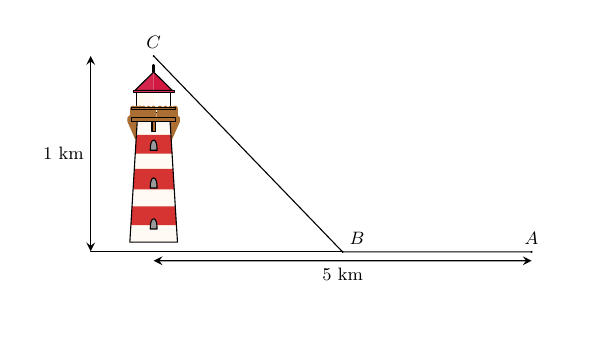
\begin{tikzpicture}[line join=round, line cap=round,scale=1,transform shape,>=stealth,scale=0.8,transform shape]
		\definecolor{anti-flashwhite}{rgb}{0.95, 0.95, 0.96}
		\definecolor{alizarin}{rgb}{0.82, 0.1, 0.26}
		\definecolor{floralwhite}{rgb}{1.0, 0.98, 0.94}
		\definecolor{brown(traditional)}{rgb}{0.59, 0.29, 0.0}
		\definecolor{bostonuniversityred}{rgb}{0.8, 0.0, 0.0}
		\definecolor{tumbleweed}{rgb}{0.87, 0.67, 0.53}%cát
		\clip (-5,-2.5) rectangle (3.5,2);
		
		\tikzset{hai_dang/.pic={
				\draw[line width=1]  (0,2.6)--(0,2.4);
				\draw[fill=alizarin] (0,2.4)--(.55,1.86)--(0,1.86);
				\draw[fill=alizarin!95] (0,2.4)--(-.55,1.86)--(0,1.86);
				\draw[fill=alizarin!90] (.6,1.86) rectangle (-.6,1.8);
				\fill[floralwhite!10] (.25,1) rectangle (.5,1.8);
				\fill[floralwhite!40] (0,1) rectangle (.25,1.8);
				\fill[floralwhite!70] (0,1) rectangle (-.25,1.8);
				\fill[floralwhite] (-.25,1) rectangle (-.5,1.8);
				\draw (-.5,1.8) rectangle (.5,1);
				\draw[fill=brown(traditional)!50] (-.55,1.2) rectangle (.55,1);
				\draw[color=brown(traditional)!80, line width=2] 
				(-.6,1)--(-.6,1.33)
				(-.5,1)--(-.5,1.33)
				(-.4,1)--(-.4,1.33)
				(-.3,1)--(-.3,1.33)
				(-.15,1)--(-.15,1.33)
				(.18,1)--(.18,1.33)
				(.35,1)--(.35,1.33)
				(.5,1)--(.5,1.33)
				(.63,1)--(.63,1.33)
				(0,1)--(0,1.33);
				\draw[color=brown(traditional)!80, line width=4] 
				(.62,1)--(.4,.5)
				(-.62,1)--(-.4,.5);
				\fill[floralwhite!70] (-.48,1)--(.48,1)--(.7,-2.6)--(-.7,-2.6)--cycle;
				\fill[bostonuniversityred!80] (-.5,.55)--(-.55,0)--(.55,0)--(.5,.55)--cycle (-.57,-.45)--(-.6,-1.05)--(.6,-1.05)--(.57,-.45)--cycle(-.64,-1.55)--(-.67,-2.1)--(.67,-2.1)--(.64,-1.55)--cycle;
				\draw (-.48,1)--(.48,1)--(.7,-2.6)--(-.7,-2.6)--cycle;
				\draw[fill=brown(traditional)!80](-.05,1) rectangle (.05,.65);
				\draw[fill=brown(traditional)!80](-.65,1.3) rectangle (.65,1.35);
				\draw[fill=brown(traditional)!80](-.65,.94) rectangle (.65,1.05);
		}}
		\tikzset{cua/.pic={
				\def\c{
					(-.1,.1)--(.1,.1)
					..controls +(88:.4) and +(92:.4) ..
					(-.1,.1)
					;}
				\draw[fill=gray!80] \c;
		}}
		\draw[<->] (-4,-1.55)--(-4,1.55);
		\node at (-4,0) [left] {\small $1$ km};
		\node at (0,-1.7) [below] {\small $5$ km};
		\draw (-4,-1.56)--(0,-1.56);
		
		\path 	(0,-1.56) coordinate (B)
		(-3,1.55) coordinate (C)
		(3,-1.56) coordinate (A)
		(3,-1.7) coordinate (A')
		;	
		\draw[<->] (-3,-1.7)--(A');
		\node at (A) [above] {\small $A$};
		\node at (B) [above right] {\small $B$};
		\node at (C) [above] {\small $C$};
		\fill[black](A) circle (.5pt);
		\fill[black](B) circle (.5pt);
		\fill[black](C) circle (.5pt);	
		\draw (A)--(B)--(C);	
		\path(-3,0)pic[scale=.6]{hai_dang};
		\path(-3,0)pic[scale=.6]{cua};
		\path(-3,-.6)pic[scale=.6]{cua};
		\path(-3,-1.25)pic[scale=.6]{cua};
\end{tikzpicture}}
	\shortans[]{$8$} 
	\loigiai{
		Gọi chiều dài đoạn dây điện kéo từ $A$ đến $B$ là $AB=x$ (km).\\
		Khi đó chiều dài dây điện kéo từ $B$ đến $C$ là $B C=\sqrt{1+(5-x)^2}=\sqrt{x^2-10x+26}$ (km).\\
		Tổng tiền công là $3\sqrt{x^2-10 x+26}+2x=13$ (triệu đồng).\\
		Theo đề bài ta có
		\begin{eqnarray*}
			&&3 \sqrt{x^2-10x+26}+2x=13 
			\Rightarrow 3 \sqrt{x^2-10 x+26}=13-2x \\
			&\Rightarrow&9\left(x^2-10x+26\right)=169-52x+4 x^2 
			\Rightarrow 5 x^2-38x + 65 = 0 \\
			&\Rightarrow  
				&\hoac{&x=5\\ &x=\dfrac{13}{5}.} 
		\end{eqnarray*}		
	   Thử lại ta thấy $x=\dfrac{13}{5}$ thỏa mãn.\\
		Khi đó $A B=x=\dfrac{13}{5}\Rightarrow BC=\dfrac{13}{5}$ (km).\\
		Khi đó tổng chiều dài dây điện đã kéo từ $A$ đến $C$ là $A B+B C=\dfrac{26}{5}=5{,}2$ (km).
	}
\end{bt}

% từ: cau-hoi/lop10/0D7_Bat_phuong_trinh_bac_2_mot_an/0D7-3-6_Toan_hinh_toan_thuc_te_ung_dung_phuong_trinh.tex
\begin{bt}%[0D7V3-6]%[ma:399b5ac6]
	Người ta muốn thiết kế một vườn hoa hình chữ nhật nội tiếp trong một miếng đất hình tròn có đường kính bằng $100$\,m. Tính diện tích vườn hoa hình chữ nhật (đơn vị: m$^2$), biết tổng quãng đường đi xung quanh vườn hoa đó là $280$\,m.
	\shortans[]{ $4800$}
	\loigiai{
		\immini{
			Gọi chiều rộng hình chữ nhật là $x=AB$\,(m).\\
			Suy ra, chiều dài hình chữ nhật là \\
			$BC=\sqrt{AC^2-AB^2}=\sqrt{10000-x^2}$\,(m).\\
			Ta có $2\left(x+\sqrt{10000-x^2}\right)=280\Leftrightarrow \sqrt{10000-x^2}=140-x$.\\
			Bình phương hai vế phương trình ta được:
			\allowdisplaybreaks
			\begin{eqnarray*}
				&&10000-x^2=(140-x)^2
				\Leftrightarrow 10000-x^2=140^2-280x+x^2
				\\
				&\Leftrightarrow& 2x^2-280x+9600=0
				\Leftrightarrow \hoac{&x=60\\&x=80.}
			\end{eqnarray*}
		}	
		{
			\begin{tikzpicture}[declare function={r=1.5;},font=\footnotesize, line join=round, line cap=round, >=stealth]
				\path (0:0) coordinate (O)
				(30:r) coordinate (A)
				(-30:r) coordinate (B)
				($(O)!-1!(A)$)  coordinate (C)
				($(O)!-1!(B)$)  coordinate (D)
				;
				\draw (A)--(B)--(C)--(D)--cycle  (A)--(C)
				(O) circle (r)
				;
				\foreach \t/\g in {A/0,B/0,C/180,D/180}{
					\draw[fill=black] (\t) circle (1pt) node[shift={(\g:7pt)},font=\scriptsize]{$ \t $};
				}
			\end{tikzpicture}
		}
		\noindent
		Thử lại, ta thấy $x=60$  và $x=80$ đều thỏa phương trình.\\
		Vậy phương trình có hai nghiệm là $\hoac{&x=60\\&x=80.}$\\
		Nếu $x=AB=60\Rightarrow BC=80$.\\
		Nếu $x=AB=80\Rightarrow BC=60$ (loại vì $BC>AB$).\\
		Vậy diện tích vườn hoa là $60\cdot 80=4\,800\,\mathrm{m}^2$.
	}
\end{bt}

% từ: cau-hoi/lop10/0D7_Bat_phuong_trinh_bac_2_mot_an/0D7-3-6_Toan_hinh_toan_thuc_te_ung_dung_phuong_trinh.tex
\begin{bt}%[0D7V3-6]%[ma:a5178634]
	\immini[thm]{
		Một người đứng ở điểm $A$ trên một bờ sông rộng $300$ m, chèo thuyền đến vị trí $D$, sau đó chạy bộ đến vị trí $B$ cách $C$ một khoảng $800$ m như bên. Vận tốc chèo thuyền là $6$ km/h, vận tốc chạy bộ là $10$ km/h và giả sử vận tốc dòng nước không đáng kể. Tính khoảng cách từ vị trí $C$ đến $D$, biết tổng thời gian người đó chèo thuyền và chạy bộ từ $A$ đến $B$ là $7{,}2$ phút.
	}
	{\begin{tikzpicture}[line join=round,line cap=round,>=stealth,font=\footnotesize,scale=.5]
			\def\d{3} %dài
			\def\r{8} %rộng
			\path 	(0:0) coordinate (E)
			++(0:\d) coordinate (B)
			++(90:\r) coordinate (C)
			++(180:\d) coordinate (A)
			($(C)!.4!(B)$) coordinate (D)
			($(A)+(0,.3)$) coordinate (A')
			($(C)+(0,.3)$) coordinate (C')
			($(A')!.5!(C')$) node[above]{\tiny $300$ m}
			($(C)+(1,0)$) coordinate (C'')
			($(B)+(1,0)$) coordinate (B')
			($(C'')!.5!(B')$) node[right]{\tiny $800$ m}
			;
			\draw (A)--(E)--(B)--(C)--cycle (D)--(A)--(B);
			\draw[<->] (A')--(C');
			\draw[<->] (B')--(C'');
			\foreach \x/ \goc in {A/135,B/-45,C/45,D/0}
			\fill (\x) circle (1pt)
			($(\x)+(\goc:4mm)$) node {$\x$};
	\end{tikzpicture}}
	\shortans[oly]{$225$}
	\loigiai{
		Theo đề bài, ta sẽ có các dữ kiện sau $1$ km/h $=\dfrac{5}{18}$ m/s.\\
		Gọi $x$ là khoảng cách từ vị trí $C$ đến $D$, theo định lý Pythagore với tam giác $ACD$, ta có $AD=\sqrt{300^2+x^2}$	(m).\\
		Khi đó thời gian để người đó chèo thuyền từ $A$ đến $D$ là $$t_{AD}=\dfrac{AD}{6\cdot\frac{5}{18}}=\dfrac{3\sqrt{300^2+x^2}}{5} \text{ (s)}.$$
		Và $DB=800-x$. Khi đó thời gian để người đó đi bộ từ $D$ đến $B$ là
		$$t_{DB}=\dfrac{DB}{10\cdot\frac{5}{18}}=\dfrac{9(800-x)}{25}\text{ (s)}.$$
		Tổng thời gian người đó chèo thuyền và chạy bộ từ $A$ đến $B$ là $7{,}2$ p$=432$ s, khi đó ta có phương trình
		\begin{eqnarray*}
			&&\dfrac{3\sqrt{300^2+x^2}}{5}+\dfrac{9(800-x)}{25}=432 \,(*)\\
			&\Leftrightarrow& 15\sqrt{90\,000+x^2}+9(800-x)=10\,800\\
			&\Leftrightarrow& \sqrt{90\,000+x^2}=\dfrac{3x}{5}+240\\
			&\Rightarrow& 90\,000+x^2=\left(\dfrac{3x}{5}+240\right)^2\\
			&\Leftrightarrow& 90\,000+x^2=\dfrac{9x^2}{25}+288x+57\,600\\
			&\Leftrightarrow& \dfrac{-16x^2}{25}+288x-32\,400=0\\
			&\Leftrightarrow& x=225.
		\end{eqnarray*}
		Thay $x=225$ vào $(*)$ thỏa mãn.\\
		Vậy khoảng cách từ vị trí $C$ đến $D$ là $225$ m.
	}
\end{bt}

% từ: cau-hoi/lop10/0D7_Bat_phuong_trinh_bac_2_mot_an/0D7-3-6_Toan_hinh_toan_thuc_te_ung_dung_phuong_trinh.tex
\begin{bt}%[0D7V3-6]%[ma:20537f22]
	\immini
	{Một người đứng ở điểm $A$ trên một bờ sông rộng $300$ m, chèo thuyền đến vị trí $D$, sau đó chạy bộ đến vị trí $B$ cách C một khoảng $800$ m như hình vẽ. Vận tốc chèo thuyền là $6$ km/h, vận tốc chạy bộ là $10$ km/h và giả sử vận tốc dòng nưốc không đáng kể. Tính khoảng cách từ vị trí $C$ đến $D$, biết tổng thời gian người đó chèo thuyền và chạy bộ từ $A$ đến $B$ là $7{,}2$ phút.}
	{
		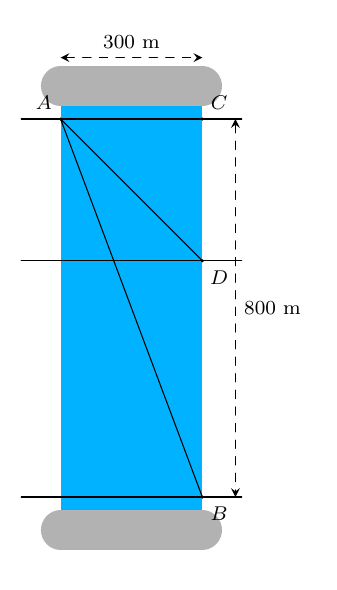
\begin{tikzpicture}[scale=0.6, font=\footnotesize, line join=round, line cap=round, >=stealth]
			\fill[blue!30!cyan] (0,-8.5) rectangle (3,0.5);
			\path 
			(0,0) coordinate (A)
			(3,0) coordinate (C)
			(3,-3) coordinate (D)
			(3,-8) coordinate (B)
			(1.5,-9) coordinate (FF) node[below]{ }
			;
			\foreach  \x in {0,-3,-8}{
				\draw[shorten <= -0.5cm,shorten >= -0.5cm,shift={(0,\x)}] (0,0)--(3,0);
			}	
			\foreach  \x in {0.7,-8.7}{
				\draw[shift={(0,\x)},line width=0.5cm,black!30] (0,0)--(3,0);
			}	
			\draw[<->,dashed] (0,1.3)--(3,1.3) node[above,midway]{$300$ m};
			\draw (B)--(A)--(D);
			\draw[<->,dashed] (3.7,0)--(3.7,-8) node[right,midway]{$800$ m};
			\foreach \p/\g in {A/135,B/-45,C/45,D/-45}\fill[black] (\p) circle (1pt) +(\g:.5)node{$\p$};
	\end{tikzpicture}}
\shortans{$225$}
	\loigiai{
		Gọi $CD=a$ km suy ra $BD=0{,}8-a$ km ($0<a< 0{,}8$).\\
		Theo giả thiết ta có $AD=\sqrt{AC^2+CD^2}=\sqrt{0{,}3^2+a^2}$.\\
		Từ đó suy ra \allowdisplaybreaks\begin{eqnarray*}
			&&\dfrac{\sqrt{0{,}3^2+a^2}}{6}+\dfrac{0{,}8-a}{10}=\dfrac{7{,}2}{60}\\
			&\Leftrightarrow & \sqrt{0{,}09+a^2}=0{,}6a+0{,}24\\
			&\Leftrightarrow & 0{,}09+a^2=0{,}36a^2+0{,}288a+0{,}0576\\
			&\Leftrightarrow & 0{,}64a^2-0{,}288a+0{,}0324=0\\
			&\Leftrightarrow & a=0{,}225.
		\end{eqnarray*}
		Vậy $CD=0{,}225$ km $=225$ m.	
	} 
\end{bt}

% từ: cau-hoi/lop10/0D7_Bat_phuong_trinh_bac_2_mot_an/0D7-3-6_Toan_hinh_toan_thuc_te_ung_dung_phuong_trinh.tex
\begin{bt}%[0D7V3-6]%[ma:b72da810]
	\immini{
		Trên bờ biển $AC$ có độ dài $80$ km. Tại hòn đảo ở vị trí $B$ cách bờ biển $AC$ một độ dài là $40$ km, một người đi xe ô tô từ vị trí $C$ với vận tốc $50$ km/h theo cung đường $AC$ và cùng lúc đó một người đi cano từ vị trí $B$ với vận tốc $70$ km/h, biết rằng $2$ người này gặp nhau tại cùng một thời điểm ở vị trí $H$ ($H$ thuộc đoạn đường $AC$). Tính quãng đường mà người tại vị trí $C$ đã di chuyển để gặp người đã di chuyển từ $B$. (Kết quả làm tròn đến hàng phần chục).
	}
	{
		\begin{tikzpicture}[font=\footnotesize,line join=round, line cap=round, >=stealth,scale=1]
			\foreach \x/\y/\pos in {0/0/A, 5/0/C} \path ($(\x,\y)$) coordinate (\pos);
			\path 
			(A)+(90:3)coordinate(B)
			($(A)!1/3!(C)$) coordinate (H)
			;
			\draw (A)--(B)node[midway,left]{$40$ km}--(H)
			(A)--(C)node[below,midway]{$80$ km}
			;
			\foreach \x/\pos in {A/180,C/0,B/90,H/60} \fill (\x) circle(1pt) node[{shift=(\pos:0.25)}]{$\x$};
		\end{tikzpicture}
	}
	\shortans{$40{,}3$}
	\loigiai{
		Gọi $x>0$ (giờ) là thời gian di chuyển của hai người.\\
		Ta có $BH=70x$; $CH=50x$.\\
		Lại có $AH=\sqrt{BH^2-AB^2}=\sqrt{4900x^2-1600}=10\sqrt{49x^2-16}$.\\
		Khi đó, $AH+CH=AC\Leftrightarrow10\sqrt{49x^2-16}+50x=80\Leftrightarrow \sqrt{49x^2-16}=8-5x$.\\
		Bình phương hai vế, ta có
		\allowdisplaybreaks
		\begin{eqnarray*}
			49x^2-16=(8-5x)^2&\Leftrightarrow&49x^2-16=64-80x+25x^2\\
			&\Leftrightarrow&24x^2+80x-80=0\\
			&\Leftrightarrow&\hoac{&x=\dfrac{-5+\sqrt{55}}{3}\\&x=\dfrac{-5-\sqrt{55}}{3}.}
		\end{eqnarray*}
		Thử lại ta nhận $x=\dfrac{-5+\sqrt{55}}{3}$.\\
		Vậy $CH=50\cdot \dfrac{-5+\sqrt{55}}{3}\approx 40{,}3$ (km).
	}
\end{bt}

% từ: cau-hoi/lop10/0H4_He_thuc_luong_trong_tam_giac/0H4-1-2_Tinh_cac_gia_tri_luong_giac.tex
\begin{ex}%[0H4N1-2]%[ma:6737e8b7]
	Giá trị của $\cos 60^\circ+\sin 30^\circ$ bằng bao nhiêu? 
	 \choice
		 {$\dfrac{\sqrt{3}}{2}$}
		{$\sqrt{3}$} 
		{$\dfrac{\sqrt{3}}{3}$} 
		{\True  $1$}
	\loigiai{ 
		Ta có $\cos  60^\circ+\sin 30^\circ=\dfrac{1}{2}+\dfrac{1}{2}=1$.
	} 
\end{ex}

% từ: cau-hoi/lop10/0H4_He_thuc_luong_trong_tam_giac/0H4-2-1_Bai_toan_chi_dung_dinh_ly_Sin_Cosin.tex
\begin{ex}%[0H4H2-1]%[ma:97507779]
	\immini[thm]{Khoảng cách từ $A$ đến $B$  không thể đo trực tiếp được vì phải đi qua một đầm lầy. Người ta xác định một điểm $C$ mà từ đó có thể nhìn được $A$ và $B$ dưới một góc $78^\circ 24'$. Biết rằng $CA=250$\,m, $CB=120$\,m. Khoảng cách $AB$ bằng bao nhiêu?
	\choice 
		{\True $255$\,m} 
		 {$166$\,m}
		 {$298$\,m}
		 {$266$\,m}}
		{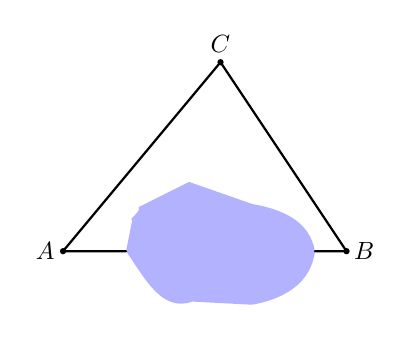
\begin{tikzpicture}[line join=round,line cap=round,>=stealth,thick,scale=0.8]
		\fill[blue!30]  (0,0)
			to[out=-55,in=200] (1.05,-0.8)--(2,-.85) 
			 to[out=10,in=263] (3,0)
			to[out=100,in=-10] (2,0.75)--(1,1.1)--(0.2,0.7) 
			 to[out=-55,in=190] (.1,0.5)--cycle;
		 \path
			(-1,0) coordinate  (A)
			 (1.5,3) coordinate (C)
			(3.5,0)  coordinate (B);
		\draw  [thick] (0,0)--(A)--(C)--(B)--(3,0);
		\foreach \i/\g in {C/90,A/180,B/0} \fill (\i) circle (.05)  node[shift={(\g:.25)}] {$\i$};
	\end{tikzpicture}
		 }
	\loigiai{ 
	Ta  có $AB=\sqrt{AC^2+BC^2-2AC\cdot BC\cdot\cos \widehat{ACB}}\approx 255$\,m.}
\end{ex}

% từ: cau-hoi/lop10/0H4_He_thuc_luong_trong_tam_giac/0H4-2-1_Bai_toan_chi_dung_dinh_ly_Sin_Cosin.tex
\begin{bt}[KNTT, Mức độ 2]%[24-25 Bài giảng K10-K11, Phan Chiến Thắng]%[0H4H2-1]%[ma:eacad5b4]
	Cho tam giác $ABC$ có $\widehat{A}=135^\circ$, $\widehat{C}=15^\circ$ và $b=12$. Tính $a,c,R$ và số đo góc $B$.
	\loigiai{Ta có $\widehat{B}=180^\circ-(\widehat{A}+\widehat{C})=30^\circ$.\\
		Áp dụng định lí sin ta có $\dfrac{a}{\sin 135^\circ}=\dfrac{12}{\sin 30^\circ}=\dfrac{c}{\sin 15^\circ}=2R$. Suy ra $a=\dfrac{12}{\sin 30^\circ}\dot\sin 135^\circ=12\sqrt{2}$.\\
		$c=\dfrac{12}{\sin 30^\circ}\dot\sin 15^\circ\approx 6{,}21$; $R=\dfrac{12}{2\sin 30^\circ}=12$.
	}
\end{bt}

% từ: cau-hoi/lop10/0H4_He_thuc_luong_trong_tam_giac/0H4-2-2_Bai_toan_co_dung_cong_thuc_dien_tich.tex
\begin{bt}%[0H4C2-2]%[ma:81cd6d13]
	 \immini[thm]
	 {
	Cho hình vẽ bên, với $M$ là điểm bên trong tam giác sao cho $\widehat{AMB}=\widehat{BMC}=\widehat{CMA}=120^{\circ}$. Đặt $MA=x$,  $MB=y$, $MC=z$. Biết các số thực dương $x$, $y$, $z$ thỏa mãn hệ phương trình $\heva{&x^2+y^2+xy=5 \\& y^2+z^2+yz=6\\ &z^2+x^2+zx=7}$. Tính giá trị biểu thức $S=xy+yz+zx$ (kết quả làm tròn đến hàng phần trăm).
	 }
	{ 
	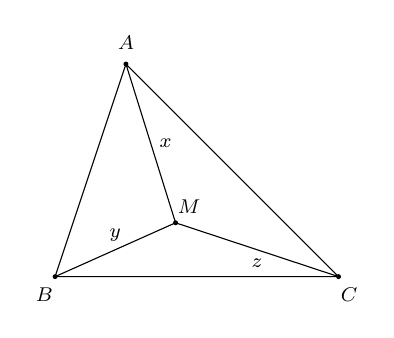
\begin{tikzpicture}[scale=0.9,font=\footnotesize,line join=round,line cap=round,>=stealth]
			 \path
				(2,4) coordinate (A) 
				(1,1) coordinate  (B)
				(5,1)  coordinate (C)
				(2.7,1.76) coordinate (M); 
			\draw (A)--(B)--(C)--(A)--(M)  node[midway,right]{$x$}
				(B)--(M) node[midway,above]{$y$} 
				(M)--(C) node[midway,below]{$z$}; 
			 \foreach \x/\g in {A/90,B/-120,C/-60,M/50}
			\fill[black] (\x)  circle (1pt)+(\g:3mm) node {$\x$};
		\end{tikzpicture}
	 }
	 \loigiai{
		Ta có $AB^2=MA^2+MB^2-2MA\cdot  MB\cdot \cos 120^\circ=x^2+y^2+xy=5\Rightarrow AB=\sqrt{5}$.\\
		Tương tự  ta tính được $BC=\sqrt{6}$, $CA=\sqrt{7}$.\\
		Đặt  $p=\dfrac{AB+BC+AC}{2}=\dfrac{\sqrt{5}+\sqrt{6}+\sqrt{7}}{2}$.\\
		Diện  tích tam giác $ABC$ là $S_{ABC}=\sqrt{p\left(p-AB\right)\left(p-AC\right)\left(p-BC\right)}=\sqrt{\dfrac{13}{2}}$.\\
		Ta có  $S_{AMB}=\dfrac{1}{2}MA \cdot MB\cdot \sin \widehat{AMB}=\dfrac{\sqrt{3}}{4}xy$, $S_{BMC}=\dfrac{\sqrt{3}}{4}yz$, $S_{CMA}=\dfrac{\sqrt{3}}{4}xz$.\\
		 Mà $S_{ABC}=S_{AMB}+S_{BMC}+S_{CMA}=\dfrac{\sqrt{3}}{4}\left(xy+yz+zx\right)$.\\
		Thế nên suy ra $xy+yz+zx=\dfrac{2\sqrt{78}}{3}\approx 5{,}89$. 
	 }
\end{bt}

% từ: cau-hoi/lop10/0H4_He_thuc_luong_trong_tam_giac/0H4-2-2_Bai_toan_co_dung_cong_thuc_dien_tich.tex
\begin{bt}%[0H4H2-2]%[Dự án đề kiểm tra Toán 10 GHKI NH23-24- Tư Đô Nguyên]%[THPT Nguyễn Du- Tp HCM]%[ma:33349022]
	\immini{
		Từ công thức diện tích $S=\dfrac{1}{2}a\cdot h_a$ của tam giác $ABC$ (tham khảo hình vẽ bên), hãy chứng minh diện tích tam giác $ABC$ còn được tính theo công thức $S=\dfrac{1}{2}ab\sin C$.%Điền câu hỏi
	}
	{
\begin{tikzpicture}[scale=1,nodes={scale=1}]
	\path (0,0) coordinate (B) 
	(4,0) coordinate (C) (1,2) coordinate (A) 
	($(B)!(A)!(C)$) coordinate (H);
	\draw (A)--(B)node[pos=.5,above left]{$c$};
	\draw (B)--(C)node[pos=.7,below]{$a$};
	\draw (C)--(A)node[pos=.5,above]{$b$};
	\draw (A)--(H)node[pos=.5,right]{$h_a$};
	\draw pic[draw,angle radius=3mm]{right angle=C--H--A};
	\foreach \x/\g in {A/90,B/180,C/-45,H/-90}
			\fill[black] 	(\x) circle (1pt)
			($(\g:3mm)+(\x)$) node {$\x$};
	\draw pic[draw,,angle radius=5mm]{angle=A--C--B};%Theo chiều dương, tùy chọn double,fill=yellow!50,-stealth,dashed

	
\end{tikzpicture}
	}
		\loigiai{
		Xét $\triangle AHC$ vuông tại $H$ ta có $\sin C=\dfrac{AH}{AC}=\dfrac{h_a}{b} \Leftrightarrow h_a=b\sin C$. \\
		Khi đó $S=\dfrac{1}{2}a\cdot h_a=\dfrac{1}{2}a \cdot \left(b \sin C\right)=\dfrac{1}{2}ab\sin C$.
	}
\end{bt}

% từ: cau-hoi/lop10/0H4_He_thuc_luong_trong_tam_giac/0H4-3-1_Giai_tam_giac.tex
\begin{bt}%[0H4H3-1]%[Dự án đề kiểm tra Toán 10 GHKI NH23-24- TheHung Nguyen]%[THPT VĨNH LỘC]%[ma:6b9a4ecb]
	Cho $\triangle ABC$ có $BC=4$cm, $ AB=2$cm, $ \widehat{B}=60^{\circ}$. Tính cạnh $AC$, $\widehat{A}$, diện tích, đường cao $AM$, bán kính đường tròn ngoại tiếp và nội tiếp của $\triangle ABC$.
	\loigiai{
	\immini{
	Theo định lý hàm số cosin ta có\\
	 $AC^2=AB^2+BC^2-2\cdot AB\cdot BC\cdot \cos B=2^2+4^2-2\cdot 2\cdot4\cdot\cos 60^\circ=12$.\\
	 Suy ra $AC=\sqrt{12}=2\sqrt{3}$.\\
	 Ta có $\heva{& BC^2=12 \\ & AC^2+AB^2=12+4=16}\Rightarrow BC^2=AC^2+AB^2$.\\
	 Suy ra $\triangle ABC$ vuông tại $A\Rightarrow \widehat{A}=90^\circ$.\\
	 Ta có $S=\dfrac{1}{2}\cdot AB\cdot AC=\dfrac{1}{2}\cdot 2\cdot 2\sqrt{3}=2\sqrt{3}$.\\
	 Ta có $S=\dfrac{1}{2}AM\cdot BC\Rightarrow AM=\dfrac{2S}{BC}=\dfrac{2\cdot 2\sqrt{3}}{4}=\sqrt{3}$.	 

}{\begin{tikzpicture}[scale=1, font=\footnotesize, line join=round, line cap=round, >=stealth]
			\draw (0,0)coordinate (A)--++(0:2)coordinate (B)--++(120:4)coordinate (C)--(A);
			\path 	($(B)!(A)!(C)$ ) coordinate (M);
			\draw (A)--(M);	
			\foreach \y/\g in {A/-180,B/0,C/90,M/10}  \fill (\y) circle (1pt)+(\g:.25)node {$\y$};
	\end{tikzpicture}}	
\noindent	Do $\triangle ABC$ vuông tại $A$ nên bán kính đường tròn ngoại tiếp  $R=\dfrac{BC}{2}=\dfrac{4}{2}=2$.	\\
Ta có $S=p\cdot r\Rightarrow r=\dfrac{S}{p}=\dfrac{2\sqrt{3}}{\dfrac{4+2+2\sqrt{2}}{2}}=\dfrac{2\sqrt{3}}{2+\sqrt{3}}=4\sqrt{3}-6$.
		
		
	}
\end{bt}

% từ: cau-hoi/lop10/0H4_He_thuc_luong_trong_tam_giac/0H4-3-1_Giai_tam_giac.tex
\begin{bt}%[0H4H3-1]%[Dự án đề kiểm tra Toán 10 GHKI NH23-24- Trương Quang Phú ]%[THPT Nguyễn Hữu Cảnh ]%[ma:4d661f2c]
\begin{enumerate}[a)]
	\item Cho $\Delta ABC$ có $BC=10$, $\widehat{A}=45^\circ$, $\widehat{B}=60^\circ$. Tính độ dài cạnh $AC$ và bán kính đường tròn ngoại tiếp $\Delta ABC$.
	\item Cho $\Delta ABC$ có $AB=5$, $BC=3$, $CA=4$. Tính giá trị $\cos A$ và độ dài đường trung tuyến $BM$ của $\Delta ABC$.
\end{enumerate}
	\loigiai{
\begin{enumerate}[a)]
	\item 
	Áp dụng định lí sin ta có $\dfrac{BC}{\sin A}=\dfrac{AC}{\sin B}\Leftrightarrow AC=BC\cdot \dfrac{\sin A}{\sin B}=\dfrac{10\sqrt{6}}{3}$.\\
	Ta có $R=\dfrac{BC}{2\sin A}=5\sqrt{2}$.
	\item Áp dụng định lí cosin ta có $\cos A=\dfrac{AB^2+AC^2-BC^2}{2AB\cdot AC}=\dfrac{4}{5}$.\\
	Ta có $BM^2=AB^2+AM^2-2\cdot AB\cdot AM\cos \widehat{BAC}=13\Rightarrow BM=\sqrt{13}$.
\end{enumerate}	
}
\end{bt}

% từ: cau-hoi/lop10/0H4_He_thuc_luong_trong_tam_giac/0H4-3-1_Giai_tam_giac.tex
\begin{bt}%[0H4H3-1]%[ma:86bba85e]
	Cho tam giác $A B C$ có $c=1, a=2$ và $\widehat{B} = 120^{\circ}$.
	\begin{enumerate}
		\item Tinh $b$, $\widehat{A}$, $\widehat{C}$.
		\item Tính diện tich của tam giác.
		\item Tính độ dài đường cao kẻ từ $B$ của tam giác.
	\end{enumerate}
	\loigiai{
		\begin{enumerate}
			\item Áp dụng định lý Cosin trong tam giác có
				$$b = \sqrt{a^2 + c^2 - 2 \cdot a \cdot c \cdot \cos \widehat{B}} = \sqrt{1 + 4- 2 \cdot 1 \cdot 2 \cdot \cos 120^{\circ}} = \sqrt{7}.$$
			Áp dụng định lý sin trong tam giác ta có
			\[\dfrac{a}{\sin A} = \dfrac{b}{\sin B} \Rightarrow \sin A = \dfrac{a \cdot \sin B}{b} = \dfrac{2 \cdot \sin 120^\circ }{\sqrt{7}}= \dfrac{\sqrt{21}}{7} \Rightarrow \widehat{A} \approx 40^\circ 54'.\]
			Suy ra $\widehat{C} \approx 19^\circ 6'$.
			\item Diện tích của tam giác là
			\[S = \dfrac{1}{2} \cdot a \cdot c \sin B  = \dfrac{1}{2} \cdot 2 \cdot 1 \cdot \sin 120^{\circ} = \dfrac{\sqrt{3}}{2} \;\;\text{(đvdt)}.\]
			\item Áp dụng công thức tính diện tích tam giác ta có
			\[S = \dfrac{1}{2} \cdot b \cdot h_b \Leftrightarrow h_b = \dfrac{2S}{b} = \dfrac{2 \cdot \dfrac{\sqrt{3}}{2}}{\sqrt{7}} = \dfrac{\sqrt{21}}{7}.\]
		\end{enumerate}
	}
\end{bt}

% từ: cau-hoi/lop10/0H4_He_thuc_luong_trong_tam_giac/0H4-3-1_Giai_tam_giac.tex
\begin{ex}%[0H4H3-1]%[ma:hl10t11]%[ma:bd30bec7]
% nguon: AI tự sinh (Ôn thi HK)
	Cho tam giác $ABC$ có $\widehat{B}=30^\circ$, $\widehat{C}=105^\circ$, $BC=10$. Xét tính đúng sai của các khẳng định sau.
	\choiceTF
		{\True $\widehat{A}=45^\circ$}
		{\True $AC=5\sqrt2$}
		{$AB=5(\sqrt6+\sqrt2)$}
		{\True $R=5\sqrt2$}
	\loigiai{
		\begin{itemchoice}
			\itemch Đúng. $\widehat{A}=180^\circ-30^\circ-105^\circ=45^\circ$.
			\itemch Đúng. $AC=\dfrac{BC\sin B}{\sin A}=\dfrac{10\cdot\frac12}{\frac{\sqrt2}{2}}=5\sqrt2$.
			\itemch Sai. $AB=\dfrac{BC\sin C}{\sin A}=\dfrac{10\sin105^\circ}{\frac{\sqrt2}{2}}$. Với $\sin105^\circ=\dfrac{\sqrt6+\sqrt2}{4}$: $AB=\dfrac{10\cdot\frac{\sqrt6+\sqrt2}{4}}{\frac{\sqrt2}{2}}=5(\sqrt3+1)$. Khẳng định sai.
			\itemch Đúng. $R=\dfrac{BC}{2\sin A}=\dfrac{10}{2\cdot\frac{\sqrt2}{2}}=5\sqrt2$.
		\end{itemchoice}
	}
\end{ex}

% từ: cau-hoi/lop11/1D1_Ham_so_luong_giac_va_phuong_trinh_luong/1D1-2-3_Bien_doi_rut_gon_bieu_thuc_luong_giac_chung_m.tex
\begin{ex}%[1D1H2-3]%[ma:6dbe7cbd]
	Rút gọn các biểu  thức sau:
	\begin{listEX}
		\item $A  = \sin (x+14^\circ) \sin (x+74^\circ) + \sin (x-76^\circ) \sin (x-16^\circ)$.
		\item $B = \dfrac{\sin (a-b)}{\cos a \cos b} + \dfrac{\sin (b-c)}{\cos  b \cos c} + \dfrac{\sin (c-a)}{\cos c \cos a}$.
	\end{listEX}
	 \loigiai{
		\begin{listEX}
			\item Ta có $A =  \sin(14^\circ + x)\cos(16^\circ - x) + \sin(76^\circ - x)\sin(16^\circ - x)$\\
			$=  \sin(14^\circ + x)\cos(16^\circ - x) + \cos(14^\circ + x)\sin(16^\circ - x)$.
			$= \sin(14^\circ + x + 16^\circ  - x) = \sin 30^\circ = \dfrac{1}{2}$.
			\item  $B = \dfrac{\sin (a-b)}{\cos a \cos b} + \dfrac{\sin (b-c)}{\cos b \cos c} + \dfrac{\sin (c-a)}{\cos c \cos a}$.\\
			Ta có $B = \dfrac{\sin a \cos b - \sin b \cos a}{\cos a \cos b} + \dfrac{\sin b \cos c - \sin c \cos b}{\cos b \cos c} + \dfrac{\sin c \cos a  - \sin a \cos c}{\cos c \cos a}$.\\
			$= \dfrac{\sin a \cos b}{\cos a \cos b} - \dfrac{\sin b \cos a}{\cos a \cos b} + \dfrac{\sin b \cos c}{\cos b \cos c} - \dfrac{\sin c \cos b}{\cos b  \cos c} + \dfrac{\sin c \cos a}{\cos c \cos a} - \dfrac{\sin a \cos c}{\cos c \cos a}$.\\
			$= \tan a - \tan b + \tan b - \tan c + \tan c  - \tan a = 0$.
		\end{listEX}
	} 
\end{ex}

% từ: cau-hoi/lop11/1D1_Ham_so_luong_giac_va_phuong_trinh_luong/1D1-2-3_Bien_doi_rut_gon_bieu_thuc_luong_giac_chung_m.tex
\begin{bt}%[1D1V2-3]%[ma:58ff5517]
% nguon: Archive/SP_KhoLatex/ID6_old/1K1-ot.tex #3782
%Câu 35
    Chứng minh biểu thức $\sin^2 x\cdot\tan x+4\sin^2 x-\tan^2 x+3\cos^2 x$ không phụ thuộc vào $x$
    \loigiai{
        \begin{eqnarray*}\sin^2 x\cdot\tan x+4\sin^2 x-\tan^2 x+3\cos^2 x&=&\left( \sin^2 x-1 \right)\tan^2 x+4\sin^2 x+3\cos^2 x\\
            &=&-\cos^2 x\cdot \tan^2 x+4\sin^2 x+3\cos^2x\\
            &=&-\sin^2 x+4\sin^2 x+3\left( 1-\sin^2 x \right)\\
            &=&3.\end{eqnarray*}}
\end{bt}

% từ: cau-hoi/lop11/1D1_Ham_so_luong_giac_va_phuong_trinh_luong/1D1-2-4_Cac_goc_luong_giac_co_lien_quan_dac_biet_bu_n.tex
\begin{bt}%[1D1N2-4]%[ma:9d1dce23]
% nguon: Archive/2024/SP-K10-K11-LyVanHoang_TVN-023/11. C1-LuongGiac-lvhoang_TVN-023/dataC1K11/Bai-1-Dang-7-GTLG-GocLienQuanDacBiet.tex #1716
[Cánh Diều, MĐ1]
	Tính 
	\begin{listEX}[2]
		\item $\sin \dfrac{13\pi}{4}$;
		\item $\sin \dfrac{\pi}{10}-\cos \dfrac{2\pi}{5}$.
	\end{listEX}
	\loigiai{
		Ta có 
		\begin{enumerate}
			\item $\sin \dfrac{13\pi}{4}=\sin \left(3\pi+\dfrac{\pi}{4}\right)=\sin \left(\pi+\dfrac{\pi}{4}\right)=-\sin \dfrac{\pi}{4}=-\dfrac{\sqrt{2}}{2}$;
			\item $\sin \dfrac{\pi}{10}-\cos \dfrac{2\pi}{5}=\sin \dfrac{\pi}{10}-\sin \left(\dfrac{\pi}{2}-\dfrac{2\pi}{5}\right)=\sin \dfrac{\pi}{10}-\sin \dfrac{\pi}{10}=0$.
		\end{enumerate}
	}
\end{bt}

% từ: cau-hoi/lop11/1D1_Ham_so_luong_giac_va_phuong_trinh_luong/1D1-2-4_Cac_goc_luong_giac_co_lien_quan_dac_biet_bu_n.tex
\begin{bt}%[1D1H2-4]%[ma:b6519b9f]
% nguon: Archive/2024/SP-K10-K11-LyVanHoang_TVN-023/11. C1-LuongGiac-lvhoang_TVN-023/dataC1K11/Bai-1-Dang-7-GTLG-GocLienQuanDacBiet.tex #1723

	Tính giá trị biểu thức $A=\cos 10^\circ+\cos 20^\circ+\ldots +\cos 90^\circ$.
	\loigiai{
		Ta có $\cos 10^\circ=-\cos 80^\circ$,..., $\cos 40^\circ=-\cos 50^\circ$. \\
		Vậy $A=\left(\cos 10^\circ+\cos 80^\circ\right)+\ldots +\left(\cos 40^\circ+\cos 50^\circ\right)+\cos 90^\circ=0$.
	}	
\end{bt}

% từ: cau-hoi/lop11/1D1_Ham_so_luong_giac_va_phuong_trinh_luong/1D1-2-4_Cac_goc_luong_giac_co_lien_quan_dac_biet_bu_n.tex
\begin{bt}%[1D1H2-4]%[ma:b54a26d6]
% nguon: Archive/SP_KhoLatex/ID6_old/1K1-1.tex #3721
%[Dự án 1 - TLDH - TeamTvdHoa - Phạm Hoàng Đăng]
	Tính giá trị các biểu thức sau
	\begin{enumerate}
		\item $A=\sin \dfrac{7\pi}{6}+\cos 9\pi +\tan\left(-\dfrac{5\pi }{4}\right)+\cot \dfrac{7\pi }{2}$.
		\item $B=\dfrac{1}{\tan 368^\circ }+\dfrac{2\sin 2550^\circ \cos (-188^\circ )}{2\cos 638^\circ +\cos 98^\circ}$.
		\item $C=\sin ^225^\circ +\sin ^245^\circ +\sin ^260^\circ +\sin ^265^\circ$.
		\item $D=\tan^2\dfrac{\pi }{8}\cdot\tan \dfrac{3\pi }{8}\cdot\tan \dfrac{5\pi}{8}$.
	\end{enumerate}
	\loigiai{
		\begin{enumerate}
			\item Ta có $A=\sin\left(\pi +\dfrac{\pi}{6}\right)+\cos (\pi +4\cdot2\pi )-\tan\left( \pi +\dfrac{\pi }{4}\right)+\cot\left( \dfrac{\pi }{2}+3\pi\right)$.\\
			$\Rightarrow A=-\sin \dfrac{\pi }{6}+\cos \pi -\tan \dfrac{\pi }{4}+\cot \dfrac{\pi }{2}=-\dfrac{1}{2}-1-1+0=-\dfrac{5}{2}$.
			\item Ta có $B=\dfrac{1}{\tan (8^\circ+360^\circ)}+\dfrac{2\sin (30^\circ+7\cdot360^\circ)\cos (8^\circ+180^\circ)}{2\cos (-90^\circ+8^\circ+2\cdot360^\circ )+\cos (90^\circ+8^\circ)}$\\
			$\begin{aligned}
				& B=\dfrac{1}{\tan 8^\circ}+\dfrac{2\sin 30^\circ(-\cos 8^\circ)}{2\cos(8^\circ-90^\circ)-\sin 8^\circ}=\dfrac{1}{\tan 8^\circ}+\dfrac{2\cdot\dfrac{1}{2}(-\cos8^\circ )}{2\cos ( 90^\circ-8^\circ)-\sin 8^\circ}\\
				&=\dfrac{1}{\tan8^\circ}-\dfrac{\cos8^\circ}{2\sin 8^\circ-\sin8^\circ}=\dfrac{1}{\tan 8^\circ}-\dfrac{\cos8^\circ}{\sin8^\circ}=0.
			\end{aligned}$
			\item Vì $25^\circ+65^\circ=90^\circ\Rightarrow \sin 65^\circ=\cos 25^\circ$ do đó \\
			$C=(\sin^2 25^\circ +\cos ^2 25)^\circ+\sin ^245^\circ +\sin ^260^\circ =1+\left(\dfrac{\sqrt{2}}{2} \right)^2+\left(\dfrac{1}{2}\right)^2$.\\
			Suy ra $C=\dfrac{7}{4}$.
			\item $D=-\left(\tan \dfrac{\pi }{8}\cdot\tan \dfrac{3\pi }{8}\right)\cdot\left[\tan\left( -\dfrac{\pi }{8}\right)\tan \dfrac{5\pi }{8}\right]$.\\
			Mà $\dfrac{\pi }{8}+\dfrac{3\pi }{8}=\dfrac{\pi }{2},\,-\dfrac{\pi }{8}+\dfrac{5\pi }{8}=\dfrac{\pi }{2}\Rightarrow \tan \dfrac{3\pi }{8}=\cot \dfrac{\pi }{8},\,\tan \dfrac{5\pi }{8}=\cot\left(-\dfrac{\pi }{8}\right).$\\
			Nên $D=-\left(\tan \dfrac{\pi }{8}\cdot\cot \dfrac{\pi }{8}\right)\cdot\left[\tan \left( -\dfrac{\pi }{8} \right)\cot\left( -\dfrac{\pi }{8}\right)\right]=-1$.
		\end{enumerate}
	}
\end{bt}

% từ: cau-hoi/lop11/1D1_Ham_so_luong_giac_va_phuong_trinh_luong/1D1-2-5_Toan_thuc_te_ap_dung_gia_tri_cua_mot_goc_luon.tex
\begin{ex}%[1D1V2-5]%[ma:2cb664f6]
	Thanh $OM$ quay ngược chiều kim đồng hồ quanh trục $O$ của nó trên một mặt phẳng thẳng đứng và in bóng vuông góc xuống mặt đất như hình bên dưới. Vị trí ban đầu của thanh là $OA$. Hỏi độ dài bóng $O'M'$ của $OM$ khi thanh quay được $5\dfrac{1}{6}$ vòng là bao nhiêu, biết độ dài thanh $OM$ là $50$ cm? (Kết quả  làm tròn đến hàng phần mười).
	\begin{center}
		\begin{tikzpicture}[scale = 0.75,font = \footnotesize,line join = round,line cap = round,> = stealth,x = 2cm,y = 2cm]
				 \def\x{1}
				 \def\a{30}
				 \pgfmathsetmacro{\y}{\x*sin (\a)}
				\pgfmathsetmacro{\z}{\x*cos  (\a)}
				\fill (0,0) node [below  right]{$O$} circle (1pt);
				 \draw[dashed](1,0) arc (0:360:2cm);
				\fill (1,0) node[above right]{$A$}circle (1pt); 
				\fill (210:1)  node[left]{$M$} circle (1pt);
				\coordinate (P) at (-1.2,-1.2); 
				 \coordinate (Q) at (1.2,-1.2);
				 \draw (1,0)--(0,0)--(210:1);
				\draw[- >]  (.2,0) arc (0:210:.4cm);
				\node  at (-.2,.2){$\alpha$};
				\coordinate (M') at ($(P)!(210:1)!(Q)$); 
				\coordinate  (O') at ($(P)!(0,0)!(Q)$);
				\foreach \i  in {M',O'}{\fill[](\i) circle (1pt);}
				\draw (P)--(Q) 
					 (210:1)--(M')
					 (0,0)--(O');
				 \foreach \i in {M',O'}{\draw (\i) node[scale = 0.9,below]{$\i$};}
				\draw[- >] (0,1.5)--(0,1.1);  \draw[- >](-0.2,1.5)--(-0.2,1.1);
				 \draw[- >](0.2,1.5)--(0.2,1.1);
				\node at (-.5,-1.3){bóng}; 
				 \node at (.8,1.3){ánh sáng};
			\end{tikzpicture}
	\end{center}
	\shortans{25} 
	 \loigiai{
		Sau khi thanh $OM$ quay được  $5$ vòng, vị trí của thanh là $OA$.\\
		Quay tiếp $\dfrac{1}{6}$, thanh sẽ tạo với  $OA$ một góc $\alpha=\dfrac{2\pi}{6}=\dfrac{\pi}{3}$.\\
	Độ dài của bóng $O'M'=OM\cos  \alpha=50 \cdot \cos \dfrac{\pi}{3}=25$ (cm).}
\end{ex}

% từ: cau-hoi/lop11/1D1_Ham_so_luong_giac_va_phuong_trinh_luong/1D1-3-2_Ap_dung_cong_thuc_cong.tex
\begin{ex}%[1D1V3-2]%[ma:b328c60c]
	Giá trị đúng của biểu thức $A=\dfrac{\tan 30^\circ+\tan 40^\circ+\tan 50^\circ+\tan 60^\circ}{\cos 20^\circ}$  bằng
	\choice 
		{$\dfrac{2}{\sqrt 3}$} 
		{$\dfrac{4}{\sqrt 3}$} 
		{$\dfrac{6}{\sqrt 3}$} 
		{\True $\dfrac{8}{\sqrt 3}$} 
	\loigiai{ 
		Ta có 
		\begin{align*}
			A&=\dfrac{\tan 30^\circ+\tan 40^\circ+\tan  50^\circ+\tan 60^\circ}{\cos 20^\circ}\\&=\dfrac{\dfrac{\sin 70^\circ}{\cos 30^\circ \cdot\cos 40^\circ}+\dfrac{\sin 110^\circ}{\cos 50^\circ \cdot\cos 60^\circ}}{\cos 20^\circ}\\
			&=\dfrac{1}{\cos 30^\circ \cdot\cos 40^\circ}+\dfrac{1}{\cos 50^\circ \cdot\cos  60^\circ}\\&=\dfrac{2}{\sqrt 3\cos 40^\circ}+\dfrac{2}{\cos 50^\circ}\\
			&=2\left(\dfrac{\cos 50^\circ+\sqrt 3\cos 40^\circ}{\sqrt 3\cos  40^\circ \cdot\cos 50^\circ}\right)\\&=2\left(\dfrac{\sin 40^\circ+\sqrt 3\cos 40^\circ}{\sqrt 3\cos 40^\circ \cdot\cos 50^\circ}\right)\\
			&=4\dfrac{\sin 100^\circ}{\dfrac{\sqrt 3}{2}\left(\cos 10^\circ+\cos 90^\circ\right)}\\&=\dfrac{8\cos 10^\circ}{\sqrt  3\cos 10^\circ}\\&=\dfrac{8}{\sqrt 3}.
		\end{align*}
	 }
\end{ex}

% từ: cau-hoi/lop11/1D1_Ham_so_luong_giac_va_phuong_trinh_luong/1D1-4-1_Cau_hoi_ly_thuyet.tex
\begin{ex}%[1D1N4-1]%[ma:9d412f1a]
	Cho đồ thị hàm số $y=\cos x$ trên đoạn $\left[-\pi;2\pi \right]$, giá trị của $x$ để hàm số  $y=\cos x$ nhận giá trị bằng 1 là
	\begin{center}
		\begin{tikzpicture}[line join=round,line cap=round,>=stealth,scale=.95,transform shape]
				\tikzset{every node/.style={font=\normalsize}} 
				\pgfmathsetmacro{\xmin}{-pi} 
				 \pgfmathsetmacro{\xmax}{2*pi}
				\def\ymin{-1.5} \def\ymax{1.5}  \def\rt{.03}
				\draw[->](\xmin-.1,0)--(\xmax+1,0) node[below]{$x$}; 
				\draw[->](0,-1.5)--(0,1.8)  node[left]{$y$};
				\draw  (0,0) node[below right]{$O$};
				\begin{scope}
					\clip (\xmin,\ymin) rectangle  (\xmax,\ymax);
					\draw[domain=\xmin:\xmax,samples=200,smooth]  plot (\x,{cos (\x r)});
				\end{scope}
				\draw[dash pattern=on 2pt off 1.5pt] 
					 (-pi,0) node[above]{-$\pi$}|-(0,-1) node[below left]{$-1$}
					(2*pi,0)  node[below]{$2\pi$}|-(0,1)
					 (pi,0) node[above]{$\pi$}|-(0,-1);
			\end{tikzpicture}
	\end{center}
	\choice 
		{$x=-\pi$} 
		{$x=\pi$} 
		{\True $x=0$} 
		 {$x=\dfrac{\pi}{2}$}
	 \loigiai{}
\end{ex}

% từ: cau-hoi/lop11/1D1_Ham_so_luong_giac_va_phuong_trinh_luong/1D1-4-4_Xet_tinh_chan_le.tex
\begin{ex}%[1D1H4-4]%[ma:149cb405]
	Cho hàm số $f(x)=\sin 2x$ và $g(x)=\tan^2 x$.  Chọn mệnh đề đúng
	 \choice
		{$f(x)$ là  hàm số chẵn, $g(x)$ là hàm số lẻ}
		{\True $f(x)$ là hàm số lẻ,  $g(x)$ là hàm số chẵn}
		{$f(x)$ là hàm số chẵn,  $g(x)$ là hàm số chẵn}
		{$f(x)$  và $g(x)$ đều là hàm số lẻ}
	\loigiai{ 
		Xét  hàm số $f(x)=\sin 2x$.
		\begin{itemize}
			\item Tập xác  định $\mathscr{D}=\mathbb{R}$. Do đó $\forall x\in \mathscr{D}\Rightarrow-x\in \mathscr{D}$.
			\item Ta có  $f\left(-x\right)=\sin \left(-2x\right)=-\sin 2x=-f(x)$.
			 $\Rightarrow f(x)$ là hàm số lẻ.
		\end{itemize}
		Xét hàm số $g(x)=\tan^2  x$.
		\begin{itemize}
			\item Tập xác định $\mathscr{D}=\mathbb{R}\setminus \left\{\dfrac{\pi}{2}+k\pi, \;k\in \mathbb{Z}\right\}$. Do đó $\forall x\in \mathscr{D}\Rightarrow-x\in \mathscr{D}$. 
			\item Ta  có $g\left(-x\right)=\left[\tan \left(-x\right)\right]^2=\left(-\tan x\right)^2=\tan^2 x=g(x)$.
			$\Rightarrow g(x)$ là hàm số  chẵn.
		\end{itemize}
	} 
\end{ex}

% từ: cau-hoi/lop11/1D1_Ham_so_luong_giac_va_phuong_trinh_luong/1D1-4-4_Xet_tinh_chan_le.tex
\begin{ex}%[1D1H4-4]%[ma:824b26bd]
	Cho hàm số  $f(x)=\sin 2x$ và $g(x)=\tan ^2x$. Chọn mệnh đề đúng?
	\choice 
		 {$f(x)$ là hàm số chẵn, $g(x)$ là hàm số lẻ}
		{\True $f(x)$ là hàm số lẻ,  $g(x)$ là hàm số chẵn}
		{$f(x)$ là hàm số chẵn, $g(x)$ là hàm số  chẵn}
		{$f(x)$ và $g(x)$  đều là hàm số lẻ}
	 \loigiai{
		Hàm  số $f(x)$ có tập xác định là $\mathscr{D}=\mathbb{R}\Rightarrow \forall x\in \mathscr{D}$ thì $-x\in \mathscr{D}$.\\
		$\forall x\in \mathscr{D}\colon f (-x)=\sin  \left(-2x\right)=-\sin 2x=-f(x)$ $\Rightarrow$ hàm số $f(x)$ là hàm số lẻ.\\
		Hàm số $g(x)$ có tập xác định là $\mathscr{D}=\mathbb{R}\setminus \left\{\dfrac{\pi}{2}+k\pi, k\in {\bf  \mathbb{Z}}\right\}$ $\Rightarrow \forall x\in \mathscr{D}$ thì $-x\in \mathscr{D}$.\\
		$\forall x\in \mathscr{D}\colon g (-x)=\tan ^2 (-x)=\tan  ^2x=g(x)$ $\Rightarrow$ hàm số $g(x)$ là hàm số chẵn.
	} 
\end{ex}

% từ: cau-hoi/lop11/1D1_Ham_so_luong_giac_va_phuong_trinh_luong/1D1-4-7_Bang_bien_thien_va_do_thi.tex
\begin{ex}%[1D1H4-7]%[ma:a339c558]
	Dùng đồ thị hàm số $y=-\sin x$ (tham khảo hình vẽ), xác định số nghiệm của phương trình $2\sin x+\sqrt{2}=0$ trên đoạn  $-\dfrac{3\pi}{2} \le x\le \dfrac{3\pi}{2}$.
	\begin{center}
		\begin{tikzpicture}[line join=round,line cap=round,>=stealth,scale=1.25,transform shape]
				\pgfmathsetmacro{\xmin}{-1.5*pi} 
				 \pgfmathsetmacro{\xmax}{1.5*pi}
				\def\ymin{-1.5} \def\ymax{1.5}  \def\rt{.03}
				\draw[->](\xmin-.1,0)--(\xmax+1,0)  node[below]{$x$};
				\draw[->](0,-1.5)--(0,1.8)  node[left]{$y$};
				 \draw (0,0) node[below left]{$O$};
				\begin{scope}
					 \clip (\xmin,\ymin) rectangle (\xmax,\ymax);
					\draw[domain=\xmin:\xmax,samples=200,smooth] plot (\x,{-sin  (\x r)});
				\end{scope}
				\draw[dash  pattern=on 2pt off 1.5pt]
					(-pi,0) node[below]{$-\pi$} 
					(pi,0) node[below]{$\pi$} 
					(-1.5*pi,0)  node[above]{-$\tfrac{3\pi}{2}$}|-(0,-1) node[below left]{$-1$}
					(1.5*pi,0) node[below]{$\tfrac{3\pi}{2}$}|-(0,1)  node[above left]{$1$}
					 (-.5*pi,0) node[below]{-$\tfrac{\pi}{2}$}|-(0,1)
					(.5*pi,0) node[below  right]{$\tfrac{\pi}{2}$}|-(0,-1);
			\end{tikzpicture}
	\end{center}
	 \choice
		 {$2$}
		{\True  $3$}
		{$1$} 
		{$4$} 
	\loigiai{ 
		Ta có: $2\sin x-\sqrt{2}=0\Leftrightarrow-\sin x=\dfrac{\sqrt{2}}{2}$. Đồ thị hàm số $y=-\sin x$ và đường thẳng $y=\dfrac{\sqrt{2}}{2}$ trên đoạn $-\dfrac{3\pi}{2} \le x\le  \dfrac{3\pi}{2}$ được vẽ như hình sau:
		\begin{center}
			\begin{tikzpicture}[line join=round,line cap=round,>=stealth,scale=1.25,transform shape]
					\pgfmathsetmacro{\xmin}{-1.5*pi} 
					\pgfmathsetmacro{\xmax}{1.5*pi} 
					 \def\ymin{-1.5} \def\ymax{1.5} \def\rt{.03}
					\draw[->](\xmin-.1,0)--(\xmax+1,0)  node[below]{$x$};
					 \draw[->](0,-1.5)--(0,1.8) node[left]{$y$};
					\draw (0,0)  node[below left]{$O$};
					\begin{scope}
						 \clip (\xmin,\ymin) rectangle (\xmax,\ymax);
						\draw[domain=\xmin:\xmax,samples=200,smooth]  plot (\x,{-sin (\x r)});
					\end{scope}
					\draw[dash pattern=on 2pt off  1.5pt]
						(-pi,0)  node[below]{$-\pi$}
						 (pi,0) node[below]{$\pi$}
						(-1.5*pi,0) node[above]{-$\tfrac{3\pi}{2}$}|-(0,-1)  node[below left]{$-1$}
						(1.5*pi,0) node[below]{$\tfrac{3\pi}{2}$}|-(0,1) node[above  left]{$1$}
						 (-.5*pi,0) node[below]{-$\tfrac{\pi}{2}$}|-(0,1)
						(.5*pi,0)  node[below right]{$\tfrac{\pi}{2}$}|-(0,-1);
					 \draw[blue](\xmin+.75,.71)--(\xmax,.71) node[above,pos=.1]{$y=\tfrac{\sqrt{2}}{2}$};
				\end{tikzpicture}
		\end{center}
		Từ đồ  thị ta thấy đường thẳng $y=\dfrac{\sqrt{2}}{2}$ cắt đồ thị hàm số $y=-\sin x$ trên đoạn $-\dfrac{3\pi}{2} \le x\le \dfrac{3\pi}{2}$ tại 3 điểm.
	} 
\end{ex}

% từ: cau-hoi/lop11/1D1_Ham_so_luong_giac_va_phuong_trinh_luong/1D1-4-7_Bang_bien_thien_va_do_thi.tex
\begin{ex}%[1D1H4-7]%[ma:a7e09934]
	Dùng đồ thị hàm số $y=\sin x$ (tham  khảo hình vẽ) để xác định số nghiệm của phương trình $2\sin x-1=0$ trên khoảng $\left(-\dfrac{\pi}{2};2\pi \right)$.
	\begin{center}
		\begin{tikzpicture}[line join=round,line cap=round,>=stealth,scale=.95,transform shape]
				\pgfmathsetmacro{\xmin}{-.5*pi} 
				 \pgfmathsetmacro{\xmax}{2*pi}
				 \def\ymin{-1.5} \def\ymax{1.5} \def\rt{.03}
				\draw[->](\xmin-.1,0)--(\xmax+1,0)  node[below]{$x$};
				\draw[->](0,-1.5)--(0,1.8) node[left]{$y$}; 
				\draw (0,0) node[below  right]{$O$};
				\begin{scope}
					\clip (\xmin,\ymin) rectangle  (\xmax,\ymax);
					\draw[domain=\xmin:\xmax,samples=200,smooth] plot (\x,{sin (\x  r)});
				\end{scope}
				 \draw[dash pattern=on 2pt off 1.5pt]
					(2*pi,0) node[above left]{$2\pi$} 
					 (pi,0) node[below left]{$\pi$}
					 (1.5*pi,0) node[above]{$\tfrac{3\pi}{2}$}|-(0,-1) node[above left]{$-1$}
					 (-.5*pi,0) node[above]{-$\tfrac{\pi}{2}$}|-(0,-1)
					(.5*pi,0) node[below]{$\tfrac{\pi}{2}$}|-(0,1) node[left]{$1$}; 
			\end{tikzpicture}
	\end{center}
	\choice 
		 {$3$}
		{\True $2$} 
		 {$1$}
		{$4$} 
	\loigiai{ 
		Ta có $2\sin  x-1=0\Leftrightarrow \sin x=\dfrac{1}{2}$.
		\begin{center}
			\begin{tikzpicture}[line join=round,line cap=round,>=stealth,scale=.95,transform shape]
					\pgfmathsetmacro{\xmin}{-.5*pi} 
					\pgfmathsetmacro{\xmax}{2*pi} 
					\def\ymin{-1.5}  \def\ymax{1.5} \def\rt{.03}
					 \draw[->](\xmin-.1,0)--(\xmax+1,0) node[below]{$x$};
					\draw[->](0,-1.5)--(0,1.8) node[left]{$y$}; 
					\draw (0,0) node[below  right]{$O$};
					\begin{scope}
						\clip  (\xmin,\ymin) rectangle (\xmax,\ymax);
						 \draw[domain=\xmin:\xmax,samples=200,smooth] plot (\x,{sin (\x r)});
					\end{scope}
					\draw[dash pattern=on 2pt  off 1.5pt]
						(2*pi,0) node[below right]{$2\pi$} 
						(pi,0)  node[below left]{$\pi$}
						(1.5*pi,0) node[below right]{$\tfrac{3\pi}{2}$}|-(0,-1)  node[above left]{$-1$}
						(-.5*pi,0) node[below  right]{-$\tfrac{\pi}{2}$}|-(0,-1)
						 (.5*pi,0) node[below]{$\tfrac{\pi}{2}$}|-(0,1) node[left]{$1$};
					\draw[blue] (\xmin,.5)--(\xmax,.5)  node[above left]{$y=\tfrac{1}{2}$};
				\end{tikzpicture}
		\end{center}
		Dựa vào đồ thị ta thấy đường thẳng $y=\dfrac{1}{2}$ cắt đồ thị  hàm số $y=\sin x$ tại hai điểm phân biệt.\\
		Vậy phương trình đã cho có hai  nghiệm phân biệt.
	} 
\end{ex}

% từ: cau-hoi/lop11/1D1_Ham_so_luong_giac_va_phuong_trinh_luong/1D1-4-7_Bang_bien_thien_va_do_thi.tex
\begin{bt}%[1D1H4-7]%[ma:49bd04db]
% nguon: Archive/2024/SP-K10-K11-LyVanHoang_TVN-023/11. C1-LuongGiac-lvhoang_TVN-023/dataC1K11/Bai-3-Dang-6-Dothihamsoluonggiac.tex #2061
%[BG K11, Nhật Thiện]
	[Mức độ 2]
	\immini{Cho đồ thị hàm số $y= 2\sin x+ 1$ như hình vẽ, dựa vào đồ thị hãy tìm
		\begin{enumerate}
			\item Giá trị lớn nhất và giá trị nhỏ nhất của hàm số trên đoạn $\left[- \pi; \pi\right]$.
			\item Các khoảng đồng biến và nghịch biến của hàm số trên đoạn $\left[- \pi; \pi\right]$.
	\end{enumerate}}
	{
		\begin{tikzpicture}[line join=round, line cap=round,>=stealth]
			%Giới hạn đồ thị và hàm số cần vẽ
			\def \xmin{-pi-1} 		\def \xmax{pi+1}
			\def \ymin{-2}		\def \ymax{4}
			\def \hamso{2*sin(\x r)+1}
			% Vẽ hệ trục
			\draw[->] (\xmin,0)--(\xmax,0) node[above right] {$x$}; 
			\draw[->] (0,\ymin)--(0,\ymax) node[below left] {$y$}; 
			\draw (0,0) node [below right] {$O$}; 
			% Vẽ các điểm trên 2 hệ trục  
			\foreach \x in {-pi,-pi/2,pi/2,pi} \draw[thin] (\x,1pt)--(\x,-1pt);
			\foreach \y in {-1,1,3} \draw[thin] (1pt,\y)--(-1pt,\y);
			\node at (-pi,0) [below]{$-\pi$};
			\node at (-pi/2,0)[above]{$-\dfrac{\pi}{2}$};
			\node at (pi,0) [below]{$\pi$};
			\node at (pi/2,0) [below]{$\dfrac{\pi}{2}$};
			\node at (0,1) [above left]{$1$};
			\node at (0,-1) [right]{$-1$};
			\node at (0,3)[left]{$3$};
			% Vẽ thêm mấy cái râu ria 
			\draw[dashed,thin](-pi/2,0)--(-pi/2,-1)--(0,-1); 
			\draw[dashed,thin](pi/2,0)--(pi/2,3)--(0,3); 
			\draw[dashed,thin] (-pi,0)--(-pi,1)--(0,1);
			\draw[dashed,thin] (pi,0)--(pi,1)--(0,1);
			% Vẽ hàm số
			\begin{scope}
				\clip (\xmin+0.1,\ymin+0.1) rectangle (\xmax-0.1,\ymax-0.1); 
				\draw[samples=350,domain=\xmin+0.1:\xmax-0.1,smooth,variable=\x] plot (\x,{\hamso}); 
			\end{scope} 
		\end{tikzpicture}
	}
	\loigiai{Dựa vào đồ thị ta có
		\begin{enumerate}
			\item
			Giá trị lớn nhất của hàm số đã cho trên đoạn $[-\pi; \pi]$ là $3$ khi $x= \dfrac{\pi}{2}$.\\
			Giá trị nhỏ nhất của hàm số đã cho trên đoạn $[-\pi; \pi]$ là $-1$ khi $x= -\dfrac{\pi}{2}$.
			\item  Trên đoạn $[-\pi;\pi]$, hàm số đã cho đồng biến trên khoảng $\left(\dfrac{-\pi}{2}; \dfrac{\pi}{2}\right)$.\\
			Trên đoạn $[-\pi;\pi]$, hàm số đã cho nghịch biến trên các khoảng $\left(-\pi; -\dfrac{\pi}{2}\right)$ và $\left(\dfrac{\pi}{2}; \pi\right).$
		\end{enumerate}
	}
\end{bt}

% từ: cau-hoi/lop11/1D1_Ham_so_luong_giac_va_phuong_trinh_luong/1D1-5-3_Phuong_trinh_co_ban_dung_Radian.tex
\begin{ex}%[1D1V5-3]%[ma:0944aac3]
	Nghiệm của phương trình $2 \sin x+1=0$ được biểu diễn trên đường tròn lượng giác ở hình bên là  những điểm nào?
	\begin{center}
		\begin{tikzpicture}[scale=0.8,font=\footnotesize,line join=round,line cap=round,>=stealth]
				 \def\r{2}
				\draw[->] (-3,0) -- (3,0) node[above] {$x$}; 
				\draw[->] (0,-3) --  (0,3) node[right] {$y$};
				\path 
					 (0:0) coordinate (O)
					(0:\r) coordinate  (A)
					(180:\r) coordinate  (A')
					(90:\r) coordinate (B) 
					(-90:\r) coordinate  (B')
					(30:\r) coordinate  (C)
					 (150:\r) coordinate (D)
					(-150:\r) coordinate  (E)
					(-30:\r) coordinate  (F);
				\draw (D)--(F) 
					(C)--(E); 
				\draw  (O) circle (\r);
				\foreach \x/\g in {A/45,B/135,C/60,D/120,A'/135,E/-150,B'/-135,F/-30,O/-120}\fill[red] (\x) circle (1pt) 
					($(\x)+(\g:4mm)$)  node{$\x$};
			\end{tikzpicture}
	\end{center}
	\choice 
		{Điểm  $D$, điểm $C$}
		 {\True Điểm $E$, điểm $F$}
		{Điểm $C$,  điểm $F$}
		{Điểm $E$, điểm $D$} 
	 \loigiai{
		Ta có $2 \sin x+1=0 
		\Leftrightarrow \sin x=-\dfrac{1}{2} \Leftrightarrow  \hoac{& x=-\dfrac{\pi}{6}+k 2 \pi \\ & x=\dfrac{7 \pi}{6}+k2\pi}(k \in \mathbb{Z})$.\\
		Với $k=0 \Rightarrow x=-\dfrac{\pi}{6}$ hoặc  $x=\dfrac{7 \pi}{6}$.\\
		Điểm biểu diễn của $x=-\dfrac{\pi}{6}$ là $F$, điểm bîểu diễn $x=\dfrac{7 \pi}{6}$  là $E$.
	 }
\end{ex}

% từ: cau-hoi/lop11/1D1_Ham_so_luong_giac_va_phuong_trinh_luong/1D1-5-3_Phuong_trinh_co_ban_dung_Radian.tex
\begin{ex}%[1D1H5-3]%[1D1H5-4]%[1D1H5-5]%[ma:e9986fe9]
	Giải các phương  trình lượng giác sau:
	\begin{multicols}{3}
		\begin{enumerate}
			 \item $\sin x=\dfrac{\sqrt{3}}{2}$;
			\item $2\cos  x=-\sqrt{2}$;
			\item  $\sqrt{3}\tan\left(\dfrac{x}{2}+15^{\circ}\right)=1$;
			\item  $\cot\left(2x-1\right)=\cot\dfrac{\pi}{5}$;
			\item  $\sin2x+\cos4x=0$;
			\item $\cos3x=-\cos7x$. 
		\end{enumerate}
	\end{multicols}
	\loigiai{ 
		\begin{enumerate}
			 \item Ta có
			\[\sin x=\dfrac{\sqrt{3}}{2} 
			\Leftrightarrow  \sin x=\sin\dfrac{\pi}{3} \Leftrightarrow
			\hoac{&x=\dfrac{\pi}{3}+k2\pi\\ 
			&x=\pi-\dfrac{\pi}{3}+k2\pi}\left(k\in \mathbb{Z}\right) 
			\Leftrightarrow 
			\hoac{&x=\dfrac{\pi}{3}+k2\pi\\ 
			&x=\dfrac{2\pi}{3}+k2\pi}\left(k\in \mathbb{Z}\right).\] 
			Vậy phương trình đã cho có các nghiệm là $x=\dfrac{\pi}{3}+k2\pi, k\in\mathbb{Z}$ và $x=\dfrac{2\pi}{3}+k2\pi, k\in\mathbb{Z}$. 
			 \item Ta có
			\[2\cos  x=-\sqrt{2}
			\Leftrightarrow \cos x=-\dfrac{\sqrt{2}}{2} 
			 \Leftrightarrow \cos x=\cos\dfrac{3\pi}{4}
			\Leftrightarrow \hoac{&x=\dfrac{3\pi}{4}+k2\pi\\ 
			&x=-\dfrac{3\pi}{4}+k2\pi}\left(k\in  \mathbb{Z}\right).\]
			Vậy phương trình đã cho có các nghiệm là $x=\dfrac{3\pi}{4}+k2\pi, k\in\mathbb{Z}$  và $x=-\dfrac{3\pi}{4}+k2\pi, k\in\mathbb{Z}$.
			\item  Ta có
			\begin{eqnarray*}
				 &&\sqrt{3} \tan\left(\dfrac{x}{2}+15^{\circ} \right)=1\\
				&\Leftrightarrow& \tan\left(\dfrac{x}{2}+15^{\circ}  \right)=\dfrac{1}{\sqrt{3}}\\
				&\Leftrightarrow&  \tan\left(\dfrac{x}{2}+15^{\circ} \right)=\tan30^{\circ}\\
				 &\Leftrightarrow& \dfrac{x}{2}+15^{\circ}=30^{\circ}+k180^{\circ}, k\in \mathbb{Z}\\
				&\Leftrightarrow&  x=30^{\circ}+k360^{\circ}, k\in \mathbb{Z}.
			\end{eqnarray*}
			Vậy phương trình đã cho có  nghiệm là $x=30^{\circ}+k360^{\circ}, k\in\mathbb{Z}$.
			\item Ta  có
			 \[\cot\left(2x-1\right)=\cot\dfrac{\pi}{5} \Leftrightarrow 2x-1=\dfrac{\pi}{5}+k\pi, k\in \mathbb{Z}\Leftrightarrow x=\dfrac{\pi}{10}+\dfrac{1}{2}+\dfrac{k\pi}{2}, k\in \mathbb{Z}.\]
			Vậy phương trình đã cho có  nghiệm là $x=\dfrac{\pi}{10}+\dfrac{1}{2}+\dfrac{k\pi}{2}, k\in\mathbb{Z}$.
			\item Ta có 
			\begin{eqnarray*}
				&&\sin2x+\cos4x=0\\ 
				 &\Leftrightarrow& \cos4x=-\sin2x\\
				&\Leftrightarrow&  \cos4x=\sin\left(-2x\right)\\
				&\Leftrightarrow& \cos4x=\cos\left[\dfrac{\pi}{2}-\left(-2x\right)\right]\\ 
				&\Leftrightarrow&  \cos4x=\cos\left(\dfrac{\pi}{2}+2x\right)\\
				 &\Leftrightarrow& \hoac{&{4x=\dfrac{\pi}{2}+2x+k2\pi} \\
				 &{4x=-\left(\dfrac{\pi}{2}+2x\right)+k2\pi}}\left(k\in \mathbb{Z}\right)\\
				&\Leftrightarrow&  \hoac{&x=\dfrac{\pi}{4}+k\pi \\
				&x=-\dfrac{\pi}{12}+\dfrac{k\pi}{3}}\left(k\in \mathbb{Z}\right). 
			\end{eqnarray*}
			Vậy phương  trình đã cho có các nghiệm là $x=\dfrac{\pi}{4}+k\pi, k\in\mathbb{Z}$ và $x=-\dfrac{\pi}{12}+\dfrac{k\pi}{3}, k\in\mathbb{Z}$.
			\item Ta  có
			\begin{eqnarray*}
				&&\cos3x=-\cos7x\\ 
				&\Leftrightarrow&  \cos3x=\cos\left(\pi+7x\right)\\
				 &\Leftrightarrow& \hoac{&3x=\pi+7x+k2\pi\\
				 &3x=-\left(\pi+7x\right)+k2\pi}\left(k\in \mathbb{Z}\right)\\
				 &\Leftrightarrow& \hoac{&{x=-\dfrac{\pi}{4}+\dfrac{k\pi}{2}} \\
				&{x=-\dfrac{\pi}{10}+\dfrac{k\pi}{5}}}\left(k\in  \mathbb{Z}\right).
			\end{eqnarray*}
			Vậy phương trình đã cho có các nghiệm là $x=-\dfrac{\pi}{4}+\dfrac{k\pi}{2}, k\in\mathbb{Z}$ và  $x=-\dfrac{\pi}{10}+\dfrac{k\pi}{5}, k\in\mathbb{Z}$.
		\end{enumerate}
	} 
\end{ex}

% từ: cau-hoi/lop11/1D1_Ham_so_luong_giac_va_phuong_trinh_luong/1D1-5-3_Phuong_trinh_co_ban_dung_Radian.tex
\begin{bt}%[1D1V5-3]%[ma:3336116f]
% nguon: Archive/SP_DA_SauLuoi/1-TL-THPT-Tenloman-GHKI-NH23-24.tex #2587
%ID%[Dự án đề kiểm tra Toán 11 GHKI NH23-24- DinhTri]%[THPT Tenloman - Tp HCM]
	Giải các phương trình lượng giác sau:
	\begin{enumerate}
		\item $\cos 2 x=\cos \dfrac{\pi}{5}$
		\item $\sin x=\cos 2 x$
	\end{enumerate}
	\loigiai{
		
		\begin{enumerate}
			\item $\cos 2x=\cos \dfrac{\pi}{5}\Leftrightarrow \hoac{&2x=\dfrac{\pi}{5}+k2\pi \\&2x=-\dfrac{\pi}{5}+k2\pi}\Leftrightarrow \hoac{&x=\dfrac{\pi}{10}+k\pi,k\in \mathbb{Z} \\&x=-\dfrac{\pi}{10}+k\pi,k\in \mathbb{Z}}$.
			\item $\cos \left(\dfrac{\pi}{2}-x\right)=\cos 2x\Leftrightarrow \hoac{&-3x=\dfrac{-\pi}{2}+k2\pi \\&x=-\dfrac{\pi}{2}+k2\pi}\Leftrightarrow \hoac{&x=\dfrac{\pi}{6}-\dfrac{k2\pi}{3},k\in \mathbb{Z} \\&x=-\dfrac{\pi}{2}+k2\pi,k\in \mathbb{Z}}$.
		\end{enumerate}
	}
\end{bt}

% từ: cau-hoi/lop11/1D1_Ham_so_luong_giac_va_phuong_trinh_luong/1D1-5-3_Phuong_trinh_co_ban_dung_Radian.tex
\begin{bt}%[1D1N5-3]%[ma:4a6a8bb1]
% nguon: Archive/2024/TOAN_11_XE/TOAN_11_XE/data4/11C1/KNTT-1.4.tex #1074
%[Tex hóa SGK 11, KNTT]
	Giải các phương trình sau
	\begin{multicols}{2}
		\begin{enumerate}
			\item  $\sin x = -\dfrac{\sqrt{3}}{2}$;
			\item $\sin x = \dfrac{1}{3}$.
		\end{enumerate}
	\end{multicols}	
	\loigiai{
		\begin{enumerate}
			\item  $\sin x = -\dfrac{\sqrt{3}}{2} \Leftrightarrow \sin x = \sin \left( -\dfrac{\pi}{3} \right) \Leftrightarrow \hoac{& x = -\dfrac{\pi}{3} + k2\pi \\ & x = \dfrac{4\pi}{3} + k2\pi } \,\, (k \in \mathbb{Z}).$
			\item Gọi $\alpha \in \left[ -\dfrac{\pi}{2}; \dfrac{\pi}{2} \right]$ là góc thỏa mãn $\sin \alpha = \dfrac{1}{3}$. Khi đó,
			$$\sin x = \dfrac{1}{3} \Leftrightarrow \sin x = \sin \alpha \Leftrightarrow \hoac{& x = \alpha + k2\pi \\ & x = \pi - \alpha + k2\pi} \,\, (k \in \mathbb{Z}).$$
		\end{enumerate}
	}
\end{bt}

% từ: cau-hoi/lop11/1D1_Ham_so_luong_giac_va_phuong_trinh_luong/1D1-5-4_Phuong_trinh_co_ban_dung_Do.tex
\begin{bt}%[1D1N5-4]%[ma:b10a2715]
% nguon: Archive/SP_SauLuoi_2024-2025/SP_GHKI/1-TL-TN-DS-NguyenThiMinhKhai-HCM-GHKI-NH24-25.tex #127

	Giải các phương trình sau:
	\begin{enumerate}
		\item $\tan \left(2x-55^{\circ}\right)=1$.
		\item $1-2\sin^2x=\cos (x-12)$.
		\item $\sin x-\sqrt{3}\cos x=-2\cos \left(3x+\dfrac{\pi}{2}\right)$.
	\end{enumerate}
\loigiai{
	\begin{enumerate}
		\item $\tan \left(2x-55^{\circ}\right)=1\Leftrightarrow 2x-55^{\circ}=45^{\circ}+k\cdot 180^{\circ}\Leftrightarrow x=50^{\circ}+k\cdot 90^{\circ}$, $k\in\mathbb{Z}$.
		\item Ta có \allowdisplaybreaks
		\begin{eqnarray*}
		& &1-2\sin^2x=\cos (x-12)\\
		&\Leftrightarrow& \cos 2x=\cos (x-12)\\
		&\Leftrightarrow&\hoac{&2x=x-12+k\cdot 2\pi\\&2x=12-x+k\cdot 2\pi}\\
		&\Leftrightarrow&\hoac{&x=-12+k\cdot 2\pi\\&x=4+k\cdot\dfrac{2\pi}{3}}, k\in\mathbb{Z}.
		\end{eqnarray*}
		\item  Ta có \allowdisplaybreaks
		\begin{eqnarray*}
			& &\sin x-\sqrt{3}\cos x=-2\cos \left(3x+\dfrac{\pi}{2}\right)\\
			&\Leftrightarrow& \dfrac{1}{2}\cdot\sin x-\dfrac{\sqrt{3}}{2}\cdot\cos x=\sin 3x\\
			&\Leftrightarrow& \sin x\cdot\cos\dfrac{\pi}{3}-\sin\dfrac{\pi}{3}\cdot\cos x=\sin 3x\\
			&\Leftrightarrow& \sin\left(x-\dfrac{\pi}{3}\right)=\sin 3x\\ 
			&\Leftrightarrow&\hoac{&x-\dfrac{\pi}{3}=3x+k\cdot 2\pi\\&x-\dfrac{\pi}{3}=\pi-3x+k\cdot 2\pi}\\
			&\Leftrightarrow&\hoac{&x=-\dfrac{\pi}{6}-k\cdot \pi\\&x=\dfrac{\pi}{3}+k\cdot\dfrac{\pi}{2}}, k\in\mathbb{Z}.
		\end{eqnarray*}
	\end{enumerate}
}
\end{bt}

% từ: cau-hoi/lop11/1D1_Ham_so_luong_giac_va_phuong_trinh_luong/1D1-5-5_Phuong_trinh_dua_ve_dang_co_ban.tex
\begin{bt}%[1D1V5-5]%[ma:b08fb9b9]
% nguon: Archive/SP_DA_SauLuoi/1-TL-THPT-NguyenThiMinhKhai-GHKI23-24.tex #2477
%[Dự án đề kiểm tra Toán 11 GHKI NH23-24- AHL]%[THPT - NguyenThiMinhKhai-HCM]
Giải các phương trình sau
\begin{multicols}{2}
\begin{enumerate}
\item $\sin 2 x=\sin \dfrac{\pi}{5}$.
\item $\cot \left(x+50^{\circ}\right)=\sqrt{3}$.
\item $\cos \left(3 x-\dfrac{\pi}{4}\right)=\cos 2 x$.
\item $\sin (x+6)=2 \cos ^2 5 x-1$.
\end{enumerate}
\end{multicols}
\loigiai{
\begin{enumerate}
\item  $\sin 2 x=\sin \dfrac{\pi}{5}$\\
$
\Leftrightarrow \hoac{ 
& 2 x = \dfrac { \pi } { 5 } + k 2 \pi  \\
& 2 x = \pi - \dfrac { \pi } { 5 } + k 2 \pi 
} \Leftrightarrow 
\hoac{
& x=\dfrac{\pi}{10}+k \pi \\
& x=\dfrac{2 \pi}{5}+k \pi
} (k \in \mathbb{Z})
$.
\item 
$  \cot \left(x+50^{\circ}\right)=\sqrt{3} \\
 \Leftrightarrow \cot \left(x+50^{\circ}\right)=\cot 30^{\circ} \\
 \Leftrightarrow x+50^{\circ}=30^{\circ}+k 180^{\circ} \\
  \Leftrightarrow x=-20^{\circ}+k 180^{\circ} \quad(k \in \mathbb{Z})
$.
\item $
 \cos \left(3 x-\dfrac{\pi}{4}\right)=\cos 2 x \\
 \Leftrightarrow \hoac{
& 3 x - \dfrac { \pi } { 4 } = 2 x + k 2 \pi  \\
& 3 x - \dfrac { \pi } { 4 } = - 2 x + k 2 \pi 
} \Leftrightarrow \hoac{
& x=\dfrac{\pi}{4}+k 2 \pi \\
& x=\dfrac{\pi}{20}+k \dfrac{2 \pi}{5}
} (k \in \mathbb{Z})
$.
\item  $\sin (x+6)=2 \cos ^2 5 x-1 \\
 \Leftrightarrow \sin (x+6)=\cos 10 x \\
 \Leftrightarrow \sin (x+6)=\sin \left(\dfrac{\pi}{2}-10 x\right) \\
 \Leftrightarrow \hoac{
& x + 6 = \dfrac { \pi } { 2 } - 1 0 x + k 2 \pi  \\
& x + 6 = \pi - \dfrac { \pi } { 2 } + 1 0 x + k 2 \pi 
} \Leftrightarrow \hoac{
& x=\dfrac{\pi}{22}-\dfrac{6}{11}+k \dfrac{2 \pi}{11} \\
& x=-\dfrac{\pi}{18}+\dfrac{2}{3}-k \dfrac{2 \pi}{9}
}(k \in \mathbb{Z})
$.
\end{enumerate}
}
\end{bt}

% từ: cau-hoi/lop11/1D1_Ham_so_luong_giac_va_phuong_trinh_luong/1D1-5-5_Phuong_trinh_dua_ve_dang_co_ban.tex
\begin{bt}%[1D1V5-5]%[ma:446501a3]
% nguon: Archive/SP_KhoLatex/ID6_old/1K1-4-5.tex #3322
%[DCHT Toán 11 - KNTT -Thọ Bùi] 
	Giải phương trình: $\tan(2x+1) + \cot x = 0$.
	\loigiai{
		Ta có: \begin{eqnarray*}
			\tan(2x+1) + \cot x = 0&\Leftrightarrow& \tan\left(2x+1\right)=-\cot x \\
			&\Leftrightarrow &\tan\left(2x+1\right)=\cot \left(-x\right) \\
			&\Leftrightarrow& \tan\left(2x+1\right)=\tan \left(\dfrac{\pi}{2}+x\right)\\
			&\Leftrightarrow& 2x+1=\dfrac{\pi}{2}+x+k\pi\\
			&\Leftrightarrow& x=\dfrac{\pi}{2}-1+k\pi, k\in\mathbb{Z}.
		\end{eqnarray*}
		
	}
\end{bt}

% từ: cau-hoi/lop11/1D1_Ham_so_luong_giac_va_phuong_trinh_luong/1D1-5-5_Phuong_trinh_dua_ve_dang_co_ban.tex
\begin{bt}%[1D1H5-5]%[ma:d35efa1c]
% nguon: Archive/SP_KhoLatex/ID6_old/1K1-4.tex #3796
%[Dự án 1 - TLDH - TeamTeXHoa - Nguyễn Cường]
	Giải các phương trình
	\begin{multicols}{2}
		\begin{enumerate}
			\item $\sin 4x=\sin\left(x+\dfrac{\pi}{3}\right)$;
			\item $\cot\left(x+30^\circ\right)=\cot\dfrac{x}{2}$;
			\item $\cos^2x=\dfrac{\sqrt{3}+2}{4}$;
			\item $\sin 2x=\cos 3x$.
		\end{enumerate}
	\end{multicols}
	\loigiai 
	{
		\begin{enumerate}
			\item $\sin 4x=\sin\left(x+\dfrac{\pi}{3}\right)\Leftrightarrow\hoac{&4x=x+\dfrac{\pi}{3}+k2\pi\\&4x=\pi-\left(x+\dfrac{\pi}{3}\right)+k2\pi}\Leftrightarrow\hoac{&x=\dfrac{\pi}{9}+\dfrac{k2\pi}{3}\\&x=\dfrac{2\pi}{15}+\dfrac{k2\pi}{5}},\,k\in\mathbb{Z}$.
			\item Điều kiện $\heva{&x+30^\circ\ne k180^\circ\\&\dfrac{x}{2}\ne n180^\circ}\Leftrightarrow\heva{&x\ne -30^\circ+k180^\circ\\&x\ne n360^\circ},\, k, n\in\mathbb{Z}$.\\			
			$\cot\left(x+30^\circ\right)=\cot\dfrac{x}{2}\Leftrightarrow x+30^\circ=\dfrac{x}{2}+k180^\circ\Leftrightarrow x=-60^\circ+k360^\circ,\,k\in\mathbb{Z}$.\\
			Vậy nghiệm của phương trình là $x=-60^\circ+k360^\circ,\,k\in\mathbb{Z}$.
			\item Ta có
			\allowdisplaybreaks
			\begin{eqnarray*}
				\cos^2x=\dfrac{\sqrt{3}+2}{4}&\Leftrightarrow&\dfrac{1+\cos 2x}{2}=\dfrac{\sqrt{3}+2}{4}\\
				&\Leftrightarrow&2\left(1+\cos 2x\right)=\sqrt{3}+2\\
				&\Leftrightarrow&\cos 2x=\dfrac{\sqrt{3}}{2}\\
				&\Leftrightarrow&\hoac{&2x=\dfrac{\pi}{6}+k2\pi\\&2x=-\dfrac{\pi}{6}+k2\pi}\\
					&\Leftrightarrow&\hoac{&x=\dfrac{\pi}{12}+k\pi\\&x=-\dfrac{\pi}{12}+k\pi},\, k\in\mathbb{Z}.
			\end{eqnarray*}
			\item Ta có
			\allowdisplaybreaks
			\begin{eqnarray*}
				\sin 2x=\cos 3x&\Leftrightarrow&\cos 3x=\cos\left(\dfrac{\pi}{2}-2x\right)\\
				&\Leftrightarrow&\hoac{&3x=\dfrac{\pi}{2}-2x+k2\pi\\&3x=-\dfrac{\pi}{2}+2x+k2\pi}\\
				&\Leftrightarrow&\hoac{&5x=\dfrac{\pi}{2}+k2\pi\\&x=-\dfrac{\pi}{2}+k2\pi}\\
				&\Leftrightarrow&\hoac{&x=\dfrac{\pi}{10}+\dfrac{k2\pi}{5}\\&x=-\dfrac{\pi}{2}+k2\pi},\, k\in\mathbb{Z}.
			\end{eqnarray*}
		\end{enumerate}
	}
\end{bt}

% từ: cau-hoi/lop11/1D1_Ham_so_luong_giac_va_phuong_trinh_luong/1D1-5-6_Toan_thuc_te_ap_dung_phuong_trinh_luong_giac.tex
\begin{bt}%[1D1H5-6]%[ma:22465806]
% nguon: Archive/2025-Sangtac/Khoi12/Data/1-CD/CD-1-OTGK1-De02.tex #5023

	\immini[thm]{Đồ thị ở hình bên mô tả sự thay đổi chiều cao của mực nước tại cảng trong vòng $24$ giờ tính từ lúc nửa đêm. Biết chiều cao của mực nước $h$ (m) theo thời gian $t$ (h) ($0\leq t\leq 24$) được cho bởi công thức $h=19+5\cos\left(\dfrac{\pi}{12}t+ \dfrac{\pi}{4}\right)$. Tìm thời điểm đầu tiên trong ngày khi chiều cao của mực nước là $14$ m.}
	{\begin{tikzpicture}[>=stealth,line join=round,line cap=round,font=\footnotesize,scale=0.55]
			\begin{scope}[scale=0.3]
				\draw [->](-1,0)--(0,0)node[above right]{$O$}--(27,0)node[below]{$t(h)$};
				\draw [->](0,-1)--(0,20)node[left]{$h(m)$};
				\draw [dashed](12,0)node[below]{$12$}|-(0,10)node[left]{$12$} (24,0)node[below]{$24$}|-(0,16)node[left]{$17$};
				\draw[smooth,samples=400,domain=0:24] plot(\x,{13+3*cos(pi/12*\x r)});
			\end{scope}
	\end{tikzpicture}}
	\shortans[0]{$9$}
	\loigiai{ 
		Do chiều cao của mực nước là $14$ m nên
		\allowdisplaybreaks 
		\begin{eqnarray*} 
			19+5\cos\left(\dfrac{\pi}{12}t+\dfrac{\pi}{4}\right)=14\\
			&\Leftrightarrow& \cos\left(\dfrac{\pi}{12}t+\dfrac{\pi}{4}\right)=-1\\ 
			&\Leftrightarrow& t=9+24k.
		\end{eqnarray*}
	Do $0\leq t\leq 24$ suy ra $t=9$.\\
		Vậy thời điểm $9$ giờ mà mực nước tại cảng là $14$ m. 
	}
\end{bt}

% từ: cau-hoi/lop11/1D1_Ham_so_luong_giac_va_phuong_trinh_luong/1D1-5-6_Toan_thuc_te_ap_dung_phuong_trinh_luong_giac.tex
\begin{bt}%[1D1H5-6]%[ma:1508ab70]
% nguon: Archive/2024/SP-K10-K11-LyVanHoang_TVN-023/11. C1-LuongGiac-lvhoang_TVN-023/dataC1K11/Chuong1-Bai4-Dang6-Toanthucte-lienmon.tex #1701
[CTST]%[Anh Duy]
	\immini{Trong hình bên, khi bàn đạp xe đạp quay, bóng $M$ của đầu trục quay dao động trên mặt đất quanh điểm $O$ theo phương trình $s=17\cos5\pi t$ với $s$ $(\mathrm{cm})$ là toạ độ của điểm $M$ trên trục $Ox$ và $t$ (giây) là thời gian bàn đạp quay. Xác định các thời điểm mà tại đó độ dài bóng $OM$ bằng $10$ $\mathrm{cm}$?}{
	\begin{tikzpicture}[line join = round, line cap=round,>=stealth,font=\footnotesize,scale=1]
		
		\draw[fill=brown] 
		(0, 0) -- (0, -0.16) -- (-0.6, -0.46) -- (-0.65, -0.88) -- (-1.65, -0.88)
		.. controls +(180:-0.1) and +(-90:0.1) .. (-1.8, -0.78) -- (-1.77, -0.44) 
		-- (-1.07, -0.44) -- (-0.07, 0.06) -- cycle;	
		
		\foreach \x in {0,-10,...,-350}
		\fill[black!30!white,rotate=\x] 
		(95:1.05)--(90:1.1)--(85:1.05)--cycle;
		\draw[black!30!white,line width=2pt] (0,0) circle(1.02cm);
		
		\draw[black,line width=2.5pt](0,0) circle(0.94cm);	
		\draw[black,line width=2pt](0,0) circle(0.65cm);
		
		\foreach \x in{0,72,144,216,288,360}
		\fill[line width=1pt,rotate=\x] 
		(0, 0) -- (0.1, 0.1) -- (0.13, 0.9) --(-0.13, 0.9) -- (-0.1, 0.1) -- (0, 0);
		
		\draw[fill=brown] 
		(0, 0) -- (0, 0.16) -- (0.6, 0.46) -- (0.65, 0.88) -- (1.65, 0.88)
		.. controls +(0:0.1) and +(90:0.1) .. (1.8, 0.78) -- (1.77, 0.44) 
		-- (1.07, 0.44) -- (0.07, -0.06) -- cycle	
		;
		
		\draw[dashed] (0,0) circle(1.1cm);
		
		\fill[black](0,0) circle(6pt);
		\fill[yellow] (0,0) circle(4pt);
		
		\draw[red,dashed,line width=1pt] 
		(0,0)--(0,-2)
		(1.05,-2)--(1.05,0.6)
		;
		\draw[black,line width=3pt] (0,0)--(1.05,0.6) (0,-2)node[below]{$O$}--(1.05,-2)node[above right]{$s$}node[below]{$M$};
		\draw[->](-2,-2)--(2.5,-2) node[below]{$x$ (cm)};
		
		\draw[->] (-2,1.55)..controls +(-120:0.5) and +(90:0.5) .. (-2.4,0.2);
		\draw[->] (-0.75,2.3)--(-0.75,1.5);\draw[->] (-0,2.3)--(-0,1.5); \draw[->] (0.75,2.3)--(0.75,1.5);
		
		\end{tikzpicture}}
	\loigiai{
		Độ dài bóng $OM$ bằng $10$ $\mathrm{cm}$ khi và chỉ khi
		\begin{eqnarray*}
			&&\hoac{&17\cos5\pi t=10\\&17\cos5\pi t=-10}\Leftrightarrow\hoac{&\cos5\pi t=\dfrac{10}{17}\\&\cos5\pi t=-\dfrac{10}{17}}\\&\Leftrightarrow&\hoac{&5\pi t=\pm\arccos\dfrac{10}{17}+k2\pi\\&5\pi t=\pm\arccos\left(-\dfrac{10}{17}\right)+k2\pi}\\&\Leftrightarrow&\hoac{&t=\pm\dfrac{1}{5\pi}\arccos\dfrac{10}{17}+\dfrac{2k}{5}\\&t=\pm\dfrac{1}{5\pi}\arccos\left(-\dfrac{10}{17}\right)+\dfrac{2k}{5}},\,k\in\mathbb{Z}.	
		\end{eqnarray*}
	}
\end{bt}

% từ: cau-hoi/lop11/1D1_Ham_so_luong_giac_va_phuong_trinh_luong/1D1-6-1_Phuong_trinh_bac_n_theo_mot_ham_so_luong_giac.tex
\begin{bt}%[1D1H6-1]%[ma:b2ec30b0]
% nguon: Archive/SP_KhoLatex/ID6_old/1K1-4-7.tex #3454

	Giải các phương trình lượng giác sau:
	\begin{listEX}[2]
		\item $2\cos{2x}-8\cos{x}+5=0$.
		%		 \dapso{$\hoac{&x=\dfrac{-\pi}{3}+k2\pi\\&x=\dfrac{\pi}{3}+k2\pi}(k\in\mathbb{Z})$}
		\item $1+\cos{2x}=2\cos{x}$.
		\item $9\sin{x}+\cos{2x}=8$.
		%		 \dapso{$x=\dfrac{\pi}{2}+k2\pi\,(k\in\mathbb{Z})$}
		\item $2+\cos{2x}+5\sin{x}=0$.
		%		 \dapso{$\hoac{&x=\dfrac{-\pi}{6}+k2\pi\\&x=\dfrac{-5\pi}{6}+k2\pi}(k\in\mathbb{Z})$}
		\item $3\sin{x}+2\cos{2x}=2$.
		%		 \dapso{$\hoac{&x=k2\pi\\&x=\arcsin{\dfrac{3}{4}}+k2\pi\\&x=-\arcsin{\dfrac{3}{4}}+\pi+k2\pi}(k\in\mathbb{Z})$}
		\item $2\cos{2x}+8\sin{x}-5=0$.
		%		 \dapso{$\hoac{&x=\dfrac{\pi}{6}+k2\pi\\&x=\dfrac{5\pi}{6}+k2\pi}(k\in\mathbb{Z})$}
	\end{listEX}
	\loigiai{
		\begin{listEX}[2]
			\item! Ta có
			$$
			2\cos{2x}-8\cos{x}+5=0 \Leftrightarrow 4\cos^2{x}-8\cos{x}+3=0.
			$$
			Đặt $t=\cos{x}\,(-1\le t\le 1)$. Khi đó, phương trình trở thành:
			$$
			4t^2-8t+3=0 \Leftrightarrow \hoac{&t=\dfrac{3}{2}\\&t=\dfrac{1}{2}.}
			$$
			Vì $-1\le t\le 1$ nên $t=\cos{x}=\dfrac{1}{2}\Leftrightarrow\hoac{&x=\dfrac{-\pi}{3}+k2\pi\\&x=\dfrac{\pi}{3}+k2\pi}(k\in\mathbb{Z})$.
			\item! Ta có
			$$
			1+\cos{2x}=2\cos{x} \Leftrightarrow 2\cos^2{x}-2\cos{x}=0.
			$$
			Đặt $t=\cos{x}\,(-1\le t\le 1)$. Khi đó, phương trình trở thành:
			$$
			2t^2-2t=0 \Leftrightarrow \hoac{&t=0\\&t=1.}
			$$
			Vì $-1\le t\le 1$ nên $\hoac{&t=\cos{x}=0\\&t=\cos{x}=1}\Leftrightarrow\hoac{&x=k2\pi\\&x=\dfrac{-\pi}{2}+k\pi}(k\in\mathbb{Z})$.
			\item!Ta có
			$$
			9\sin{x}+\cos{2x}=8
			\Leftrightarrow -2\sin^2{x}+9\sin{x}-7=0.
			$$
			Đặt $t=\sin{x}(-1\le t\le 1)$. Khi đó, phương trình trở thành:
			$$
			2t^2-9t+7=0 \Leftrightarrow \hoac{&t=1\\&t=\dfrac{7}{2}.}
			$$
			Vì $-1\le t\le 1$ nên $t=\sin{x}=1\Leftrightarrow x=\dfrac{\pi}{2}+k2\pi\,(k\in\mathbb{Z})$.
			\item! Ta có
			$$
			2+\cos{2x}+5\sin{x}=0 \Leftrightarrow -2\sin^2{x}+5\sin{x}+3=0.
			$$
			Đặt $t=\sin{x}(-1\le t\le 1)$. Khi đó, phương trình trở thành:
			$$
			2t^2-5t-3=0 \Leftrightarrow \hoac{&t=3\\&t=\dfrac{-1}{2}.}
			$$
			Vì $-1\le t\le 1$ nên $t=\sin{x}=\dfrac{-1}{2}\Leftrightarrow\hoac{&x=\dfrac{-\pi}{6}+k2\pi\\&x=\dfrac{-5\pi}{6}+k2\pi}(k\in\mathbb{Z})$.
			\item! Ta có
			$$
			3\sin{x}+2\cos{2x}=2 \Leftrightarrow -4\sin^2{x}+3\sin{x}=0.
			$$
			Đặt $t=\sin{x}\,(-1\le t\le 1)$. Khi đó, phương trình trở thành:
			$$
			-4t^2+3t=0 \Leftrightarrow \hoac{&t=0\\&t=\dfrac{3}{4}.}
			$$
			Vì $-1\le t\le 1$ nên $\hoac{&t=\sin{x}=0\\&t=\sin{x}=\dfrac{3}{4}}\Leftrightarrow \hoac{&x=k\pi\\&x=\arcsin{\dfrac{3}{4}}+k2\pi\\&x=-\arcsin{\dfrac{3}{4}}+\pi+k2\pi}(k\in\mathbb{Z})$.
			\item! Ta có
			$$
			2\cos{2x}+8\sin{x}-5=0 \Leftrightarrow -4\sin^2{x}+8\sin{x}-3=0.
			$$
			Đặt $t=\sin{x}\,(-1\le t\le 1)$. Khi đó, phương trình trở thành:
			$$
			4t^2-8t+3=0 \Leftrightarrow \hoac{&t=\dfrac{3}{2}\\&t=\dfrac{1}{2}.}
			$$
			Vì $-1\le t\le 1$ nên $t=\sin{x}=\dfrac{1}{2}\Leftrightarrow\hoac{&x=\dfrac{\pi}{6}+k2\pi\\&x=\dfrac{5\pi}{6}+k2\pi}(k\in\mathbb{Z})$.
		\end{listEX}
	}
\end{bt}

% từ: cau-hoi/lop11/1D1_Ham_so_luong_giac_va_phuong_trinh_luong/1D1-6-1_Phuong_trinh_bac_n_theo_mot_ham_so_luong_giac.tex
\begin{bt}%[1D1V6-1]%[ma:bdd777bd]
% nguon: Archive/SP_KhoLatex/ID6_old/1K1-4-7.tex #3456

	Giải các phương trình lượng giác sau
	\begin{listEX}[2]
		\item $3\sin^2{x}+2\cos^4{x}-2=0$.
		%		 \dapso{$\hoac{&x=k2\pi\\&x=\dfrac{-\pi}{4}+k\pi\\&x=\dfrac{\pi}{4}+k\pi}(k\in\mathbb{Z})$}
		\item $4\sin^4{x}+2\cos^2{x}=7$.
		%		 \dapso{$\hoac{&x=\dfrac{\pi}{4}+k\pi\\&x=\dfrac{-\pi}{4}+k\pi}(k\in\mathbb{Z})$}
		\item $4\cos^4{x}=4\sin^2{x}-1$
		%		 \dapso{$\hoac{&x=\dfrac{-3\pi}{4}+k\pi\\&x=\dfrac{3\pi}{4}+k\pi}(k\in\mathbb{Z})$}
		\item $4\sin^4{x}+5\cos^2{x}-4=0$
		%		 \dapso{$\hoac{&x=\dfrac{-\pi}{6}+k2\pi\\&x=\dfrac{\pi}{6}+k2\pi\\&x=k2\pi}(k\in\mathbb{Z})$}
	\end{listEX}
	\loigiai{
		\begin{listEX}[2]
			\item! Ta có
			$$
			3\sin^2{x}+2\cos^4{x}-2=0 \Leftrightarrow 2\cos^4{x}-3\cos^2{x}+1=0.
			$$
			Đặt $t=\cos^2{x}\,(0\le t\le 1)$. Khi đó, phương trình trở thành:
			$$
			2t^2-3t+1=0 \Leftrightarrow \hoac{&t=1\\&t=\dfrac{1}{2}.}
			$$
			Vì $0\le t\le 1$ nên $\hoac{&t=\cos^2{x}=1\\&t=\cos^2{x}=\dfrac{1}{2}}\Leftrightarrow\hoac{&\cos{x}=1\\&\cos{x}=\pm\dfrac{\sqrt{2}}{2}}\Leftrightarrow\hoac{&x=k2\pi\\&x=\dfrac{-\pi}{4}+k\pi\\&x=\dfrac{\pi}{4}+k\pi}(k\in\mathbb{Z})$.
			\item! Ta có
			$$
			4\sin^4{x}+12\cos^2{x}=7 \Leftrightarrow 4\sin^4{x}-12\sin^2{x}+5=0.
			$$
			Đặt $t=\sin^2{x}(0\le t\le 1)$. Khi đó, phương trình trở thành:
			$$
			4t^2-12t+5=0 \Leftrightarrow \hoac{&t=\dfrac{1}{2}\\&t=\dfrac{5}{2}.}
			$$
			Vì $0\le t\le 1$ nên $t=\sin^2{x}=\dfrac{1}{2}\Leftrightarrow\sin{x}=\pm\dfrac{\sqrt{2}}{2}\Leftrightarrow\hoac{&x=\dfrac{\pi}{4}+k\pi\\&x=\dfrac{-\pi}{4}+k\pi}(k\in\mathbb{Z})$.
			\item! Ta có
			$$
			4\cos^4{x}=4\sin^2{x}-1 \Leftrightarrow 4\cos^4{x}+4\cos^2{x}-3=0.
			$$
			Đặt $t=\cos^2{x}\,(0\le t\le 1)$. Khi đó, phương trình trở thành:
			$$
			4t^2+4t-3=0 \Leftrightarrow \hoac{&t=\dfrac{1}{2}\\&t=\dfrac{-3}{2}.}
			$$
			Vì $0\le t\le 1$ nên $t=\cos^2{x}=\dfrac{1}{2}\Leftrightarrow\cos{x}=\pm\dfrac{\sqrt{2}}{2}\Leftrightarrow\hoac{&x=\dfrac{-3\pi}{4}+k\pi\\&x=\dfrac{3\pi}{4}+k\pi}(k\in\mathbb{Z})$.
			\item! Ta có
			$$
			4\sin^4{x}+5\cos^2{x}-4=0 \Leftrightarrow 4\sin^4{x}-5\sin^2{x}+1=0.
			$$
			Đặt $t=\sin^2{x}\,(0\le t\le 1)$. Khi đó, phương trình trở thành:
			$$
			4t^2-5t+1=0 \Leftrightarrow \hoac{&t=\dfrac{1}{4}\\&t=1.}
			$$
			Vì $0\le t\le 1$ nên $\hoac{&t=\sin^2{x}=\dfrac{1}{4}\\&t=\sin^2{x}=1}\Leftrightarrow\hoac{&t=\sin{x}=\dfrac{1}{2}\\&t=\sin{x}=1}\Leftrightarrow\hoac{&x=\dfrac{5\pi}{6}+k2\pi\\&x=\dfrac{\pi}{6}+k2\pi\\&x=\dfrac{\pi}{2}+k2\pi}(k\in\mathbb{Z})$.
		\end{listEX}
	}
\end{bt}

% từ: cau-hoi/lop11/1D2_Day_so_Cap_so_cong_Cap_so_nhan/1D2-1-4_Day_so_tang_day_so_giam.tex
\begin{bt}%[1D2H1-4]%[ma:bcd8945e]
% nguon: Archive/SP_KhoLatex/ID6_old/1K2-5.tex #3376
%[Dự án 2 - TLDH - TeamTeXHoa - Nguyễn Cường]
	Xét tính đơn điệu của các dãy số sau
	\begin{multicols}{2}
		\begin{enumerate}
			\item $u_n=2n+3$;
			\item $u_n=\dfrac{\sqrt{n}}{2^n}$.
		\end{enumerate}
	\end{multicols}
	\loigiai 
	{
	\begin{enumerate}
		\item Ta có $u_n=2n+3$ và $u_{n+1}=2(n+1)+3=2n+5$.\\
		Do đó, với mọi $n\in \mathbb{N}^*$, ta có $u_{n+1}-u_n=2n+5-2n-3=2>0$.\\
		Suy ra dãy số đã cho là dãy số tăng.
		\item Ta có $u_n=\dfrac{\sqrt{n}}{2^n}$ và $u_{n+1}=\dfrac{\sqrt{n+1}}{2^{n+1}}$.\\
		Do đó, với mọi $n\in \mathbb{N}^*$, ta có $\dfrac{u_{n+1}}{u_n}=\dfrac{\sqrt{n+1}}{2^{n+1}}\cdot \dfrac{2^n}{\sqrt{n}}=\dfrac{1}{2}\sqrt{\dfrac{n+1}{n}}$.\\
		Giả sử $\dfrac{1}{2}\sqrt{\dfrac{n+1}{n}}>1\Leftrightarrow\dfrac{1}{4}\cdot\dfrac{n+1}{n}>1\Leftrightarrow n+1>4n\Leftrightarrow 3n<1$ (vô lý).\\
		Vậy $\dfrac{u_{n+1}}{u_n}<1$. Suy ra dãy số đã cho là dãy số giảm.
	\end{enumerate}
	}
\end{bt}

% từ: cau-hoi/lop11/1D2_Day_so_Cap_so_cong_Cap_so_nhan/1D2-2-2_Nhan_dien_cap_so_cong_cong_sai.tex
\begin{ex}%[1D2V2-2]%[ma:3eb70609]
	Giải phương trình sau  $2+7+12+\cdots+x=245$.
	 \shortans{47}
	 \loigiai{
		Ta có dãy số $2,7,12,\ldots, x$ lập thành cấp số cộng  có $\heva{&{u_1=2} \\
		 &{d=5} \\
		&{u_n=x}  \\
		 &{S_n=245}.
		}$\\ 
		 Suy ra $S_n=245\Leftrightarrow 245=\dfrac{n}{2} \left[2u_1+(n-1)d\right]\Leftrightarrow 245.2=n[2.2+(n-1)5]\Rightarrow n=10$.\\
		Vậy  $x=u_{10}=u_1+9d=47$.
	} 
\end{ex}

% từ: cau-hoi/lop11/1D2_Day_so_Cap_so_cong_Cap_so_nhan/1D2-2-6_Tinh_tong_cua_cap_so_cong.tex
\begin{ex}%[1D2H2-6]%[ma:92177595]
	 Giải phương trình sau $(2x+1)+(2x+6)+(2x+11)+\cdots+(2x+96)=1010$.
	 \shortans{1}
	\loigiai{ 
		Ta có dãy số $(2x+1)$, $(2x+6)$, $(2x+11)$,$\ldots, (2x+96)$ lập thành cấp  số cộng có $\heva{&{u_1=2x+1} \\
		&{d=5} \\ 
		&{u_n=2x+96} \\ 
		 &{S_n=1010}.
		}$\\ 
		Suy ra  $2x+96=2x+1+(n-1)5\Rightarrow n=20$.\\
		Vậy $S_{20}=1010\Leftrightarrow \dfrac{20}{2}  \left(u_1+u_n \right)=1010\Leftrightarrow 10(2x+1+2x+96)=1010\Rightarrow x=1$.
	} 
\end{ex}

% từ: cau-hoi/lop11/1D2_Day_so_Cap_so_cong_Cap_so_nhan/1D2-3-8_Toan_thuc_te_ap_dung_cap_so_nhan.tex
\begin{bt}%[1D2V3-8]%[ma:a9efbd3a]
	\textbf{(0.5  điểm)}Cho hình vuông ${{A}_{1}}{{B}_{1}}{{C}_{1}}{{D}_{1}}$ có độ dài đường chéo bằng $2\sqrt{6}$ (đơn vị độ dài). Chia hình vuông ${{A}_{1}}{{B}_{1}}{{C}_{1}}{{D}_{1}}$ thành $9$ hình vuông nhỏ bằng nhau và tô màu như hình vẽ bên dưới. Với ${{A}_{2}}{{B}_{2}}{{C}_{2}}{{D}_{2}}$ là hình vuông nhỏ chính giữa, lại chia thành $9$ hình vuông nhỏ bằng nhau và tô màu như quy luật trên. Cứ tiếp tục như vậy.
	\begin{center}
		{\begin{tikzpicture}[>=stealth,line join=round,line cap=round,font=\footnotesize,scale=1.3]
		 \draw (0,0)--(0,3)-- (3,3)--(3,0)--(0,0);
		\fill (0,0) circle (1.2pt)  node[below left]{$B_1$};
		\fill (0,3)  circle (1.2pt) node[above left]{$A_1$};
		\fill (3,3) circle  (1.2pt) node[above right]{$D_1$};
		\fill (3,0) circle (1.2pt) node[below right]{$C_1$}; 
		\draw (1.5,-.6) node{\textbf{}}; 
	\end{tikzpicture}
		} 
		{\begin{tikzpicture}[>=stealth,line join=round,line cap=round,font=\footnotesize,scale=1.3]
		\draw (0,3)--(1,2) 
			(3,0)--(2,1); 
		\draw[dashed]  (1,2)--(2,1);
		\fill[pattern=crosshatch dots  light steel blue,smooth] (0,3)--(0,0)--(3,0)--(2,1)--(1,1)--(1,2)--(0,3);
		\draw [step=1,very  thin] (0,0) grid (3,3);
		\fill (0,0) circle (1.2pt)  node[below left]{$B_1$};
		\fill  (0,3) circle (1.2pt) node[above left]{$A_1$};
		\fill (3,3) circle (1.2pt) node[above right]{$D_1$}; 
		\fill (3,0)  circle (1.2pt) node[below right]{$C_1$};
		\fill (1,1)  circle (1.2pt) node[above left]{$B_2$};
		 \fill (1,2) circle (1.2pt) node[above right]{$A_2$};
		\fill (2,2) circle (1.2pt)  node[above right]{$D_2$};
		\fill (2,1)  circle (1.2pt) node[above right]{$C_2$};
		\draw  (1.5,-.5) node{\textbf{Hình 1}};
	\end{tikzpicture}
		} 
		{\begin{tikzpicture}[>=stealth,line join=round,line cap=round,font=\footnotesize,scale=1.3]
		\draw (0,3)--(1.3333333,1.6666667) 
			 (3,0)--(1.6666667,1.3333333);
		\draw[dashed]  (1,2)--(2,1);
		\fill[pattern=crosshatch dots light steel blue,smooth] (0,3)--(0,0)--(3,0)--(2,1)--(1,1)--(1,2)--(0,3); 
		 \fill[pattern=crosshatch dots light steel blue,smooth] (1,2)--(1,1)--(2,1)--(1.6666667,1.3333333)--(1.3333333,1.3333333)--(1.3333333,1.6666667)--(1,2);
		\draw [step=1,very thin] (0,0) grid  (3,3);
		 \draw [step=1/3,very thin] (1,1) grid (2,2);
		\fill (0,0)  circle (1.2pt) node[below left]{$B_1$};
		\fill (0,3) circle (1.2pt)  node[above left]{$A_1$};
		\fill (3,3)  circle (1.2pt) node[above right]{$D_1$};
		 \fill (3,0) circle (1.2pt) node[below right]{$C_1$};
		\fill  (1,1) circle (1.2pt) node[above left]{$B_2$};
		\fill (1,2)  circle (1.2pt) node[above right]{$A_2$};
		\fill (2,2)  circle (1.2pt) node[above right]{$D_2$};
		\fill (2,1) circle (1.2pt) node[above  right]{$C_2$};
		\draw (1.5,-.5)  node{\textbf{Hình 2}};
	\end{tikzpicture}
		 }
	\end{center}
	\begin{enumerate}
		\item Tính diện tích phần đã  tô màu ở \textbf{Hình 1}.
		\item Gọi ${{u}_{1}},{{u}_{2}},\ldots $ lần lượt là diện tích phần tô màu ở hình vuông ${{A}_{1}}{{B}_{1}}{{C}_{1}}{{D}_{1}}$, ${{A}_{2}}{{B}_{2}}{{C}_{2}}{{D}_{2}},\ldots $ Đặt  ${{S}_{n}}={{u}_{1}}+{{u}_{2}}+\cdots +{{u}_{n}}$, tính $\lim {{S}_{n}}$.
	\end{enumerate}
	\loigiai{ 
		\begin{enumerate}
			\item Độ dài  cạnh hình vuông ban đầu đã cho: $2\sqrt{3}$ (đơn vị độ dài)\\
			Diện tích phần đã tô màu lần chia hình đầu tiên:  $4.{{\left( \dfrac{2\sqrt{3}}{3} \right)}^{2}}=\dfrac{16}{3}$.
			\item Theo đề bài, ${{S}_{n}}$ là tổng cấp số nhân với  ${{u}_{1}}=\dfrac{16}{3}$ và công bội $q=\dfrac{1}{9}$, do đó
			$${{S}_{n}}=\dfrac{16}{3}\cdot \dfrac{1-{{\left( \dfrac{1}{9} \right)}^{n}}}{1-\dfrac{1}{9}}=6\cdot \left[1-{{\left( \dfrac{1}{9} \right)}^{n}} \right].$$  Vậy $\lim {{S}_{n}}=6$.
		\end{enumerate}
	} 
\end{bt}

% từ: cau-hoi/lop11/1D2_Day_so_Cap_so_cong_Cap_so_nhan/1D2-3-8_Toan_thuc_te_ap_dung_cap_so_nhan.tex
\begin{ex}%[1D2V3-8]%[ma:026aae59]
	\textbf{(0.5 điểm)}Cho hình vuông ${{A}_{1}}{{B}_{1}}{{C}_{1}}{{D}_{1}}$ có độ dài  đường chéo bằng $2\sqrt{6}$ (đơn vị độ dài). Chia hình vuông ${{A}_{1}}{{B}_{1}}{{C}_{1}}{{D}_{1}}$ thành $9$ hình vuông nhỏ bằng nhau và tô màu như hình vẽ bên dưới. Với ${{A}_{2}}{{B}_{2}}{{C}_{2}}{{D}_{2}}$ là hình vuông nhỏ chính giữa, lại chia thành $9$ hình vuông nhỏ bằng nhau và tô màu như quy luật trên. Cứ tiếp tục như vậy.
	\begin{center}
		{\begin{tikzpicture}[>=stealth,line join=round,line cap=round,font=\footnotesize,scale=1.3]
		\draw (0,0)--(0,3)--  (3,3)--(3,0)--(0,0);
		\fill (0,0) circle (1.2pt)  node[below left]{$B_1$};
		 \fill (0,3) circle (1.2pt) node[above left]{$A_1$};
		\fill (3,3)  circle (1.2pt) node[above right]{$D_1$};
		\fill (3,0) circle (1.2pt) node[below right]{$C_1$}; 
		 \draw (1.5,-.6) node{\textbf{}};
	\end{tikzpicture}
		} 
		{\begin{tikzpicture}[>=stealth,line join=round,line cap=round,font=\footnotesize,scale=1.3]
		 \draw (0,3)--(1,2)
			(3,0)--(2,1); 
		\draw[dashed] (1,2)--(2,1); 
		\fill[pattern=crosshatch dots  light steel blue,smooth] (0,3)--(0,0)--(3,0)--(2,1)--(1,1)--(1,2)--(0,3);
		\draw [step=1,very thin]  (0,0) grid (3,3);
		\fill (0,0) circle (1.2pt) node[below left]{$B_1$}; 
		\fill (0,3) circle (1.2pt) node[above left]{$A_1$}; 
		\fill (3,3) circle (1.2pt)  node[above right]{$D_1$};
		\fill (3,0) circle  (1.2pt) node[below right]{$C_1$};
		 \fill (1,1) circle (1.2pt) node[above left]{$B_2$};
		\fill (1,2)  circle (1.2pt) node[above right]{$A_2$};
		\fill (2,2) circle  (1.2pt) node[above right]{$D_2$};
		\fill (2,1)  circle (1.2pt) node[above right]{$C_2$};
		 \draw (1.5,-.5) node{\textbf{Hình 1}};
	\end{tikzpicture}
		 }
		{\begin{tikzpicture}[>=stealth,line join=round,line cap=round,font=\footnotesize,scale=1.3]
		\draw  (0,3)--(1.3333333,1.6666667)
			(3,0)--(1.6666667,1.3333333); 
		 \draw[dashed] (1,2)--(2,1);
		\fill[pattern=crosshatch dots  light steel blue,smooth] (0,3)--(0,0)--(3,0)--(2,1)--(1,1)--(1,2)--(0,3);
		\fill[pattern=crosshatch dots light steel blue,smooth] (1,2)--(1,1)--(2,1)--(1.6666667,1.3333333)--(1.3333333,1.3333333)--(1.3333333,1.6666667)--(1,2); 
		\draw [step=1,very thin] (0,0) grid  (3,3);
		\draw [step=1/3,very thin] (1,1) grid  (2,2);
		\fill (0,0) circle  (1.2pt) node[below left]{$B_1$};
		\fill (0,3) circle (1.2pt)  node[above left]{$A_1$};
		\fill (3,3)  circle (1.2pt) node[above right]{$D_1$};
		\fill (3,0) circle (1.2pt) node[below  right]{$C_1$};
		\fill (1,1) circle (1.2pt)  node[above left]{$B_2$};
		\fill (1,2) circle (1.2pt) node[above right]{$A_2$}; 
		\fill (2,2)  circle (1.2pt) node[above right]{$D_2$};
		\fill (2,1) circle (1.2pt)  node[above right]{$C_2$};
		\draw (1.5,-.5) node{\textbf{Hình  2}};
	\end{tikzpicture}
		 }
	\end{center}
	\begin{enumerate}
		\item Tính diện tích phần đã tô màu ở  \textbf{Hình 1}.
		\item Gọi ${{u}_{1}},{{u}_{2}},\ldots $  lần lượt là diện tích phần tô màu ở hình vuông ${{A}_{1}}{{B}_{1}}{{C}_{1}}{{D}_{1}}$, ${{A}_{2}}{{B}_{2}}{{C}_{2}}{{D}_{2}},\ldots $ Đặt ${{S}_{n}}={{u}_{1}}+{{u}_{2}}+\cdots +{{u}_{n}}$, tính $\lim {{S}_{n}}$.
	\end{enumerate}
	 \loigiai{
		\begin{enumerate}
			\item Độ dài cạnh hình vuông ban đầu đã cho: $2\sqrt{3}$ (đơn vị độ  dài)\\
			Diện tích phần đã tô màu lần chia hình  đầu tiên: $4.{{\left( \dfrac{2\sqrt{3}}{3} \right)}^{2}}=\dfrac{16}{3}$.
			\item Theo đề bài, ${{S}_{n}}$ là tổng cấp số nhân với ${{u}_{1}}=\dfrac{16}{3}$ và công bội $q=\dfrac{1}{9}$,  do đó
			$${{S}_{n}}=\dfrac{16}{3}\cdot \dfrac{1-{{\left( \dfrac{1}{9} \right)}^{n}}}{1-\dfrac{1}{9}}=6\cdot \left[1-{{\left(  \dfrac{1}{9} \right)}^{n}} \right].$$ Vậy $\lim {{S}_{n}}=6$.
		\end{enumerate}
	} 
\end{ex}

% từ: cau-hoi/lop11/1D3_Gioi_han_Ham_so_lien_tuc/1D3-1-5_Cap_so_nhan_lui_vo_han.tex
\begin{bt}%[1D3V1-5]%[ma:bda5cb7b]
% nguon: Archive/SP_KhoLatex/ID6_old/1-CK1-OT-De-35.tex #2638

 Cho hình vuông $(C_1)$ có cạnh bằng $a$. Người ta chia mỗi cạnh của hình vuông thành bốn phần bằng nhau và nối các điểm chia một cách thích hợp để có hình vuông $(C_2)$ (Hình vẽ).
 \begin{center}
 \begin{tikzpicture}
 		\def\n{7} % số lần lặp hình vuông
 		\def\pos{0.25} % vị trí 
 		\def\r{6cm}
 		\path 
 		(0,0) coordinate (A)
 		++(0:\r) coordinate (B)
 		++(90:\r) coordinate (C)
 		++(180:\r) coordinate (D)
 		;
 		\foreach \i in {1,2,...,\n}{
 		\draw (A)--(B)--(C)--(D)--cycle;
 		\path (A) coordinate (X)
 		(barycentric cs:A=\pos,B=1-\pos) coordinate(A)
 		(barycentric cs:B=\pos,C=1-\pos) coordinate(B)
 		(barycentric cs:C=\pos,D=1-\pos) coordinate(C)
 		(barycentric cs:D=\pos,X=1-\pos) coordinate(D);
 		}
 	\end{tikzpicture}
 \end{center}
 Từ hình vuông $(C_2)$ lại tiếp tục làm như trên ta nhận được dãy các hình vuông $(C_1)$, $(C_2)$ ,$(C_3), \ldots$, $(C_n)$. Gọi $S_i$ là diện tích của hình vuông $C_i~(i\in\{1;2;3\ldots;n\})$. Đặt $T=S_1+S_2+S_3+\cdots+S_n+\cdots$ Biết $T=\dfrac{32}{3}$. Tìm $a$.
 \loigiai{
 Cạnh của hình vuông $\left(C_2 \right)$ là $a_2=\sqrt{\left(\dfrac{3}{4} a\right)^2+\left(\dfrac{1}{4} a\right)^2}=\dfrac{a\sqrt{10}}{4}$.\\ 
 Do đó diện tích $S_2=\dfrac{5}{8} a^2=\dfrac{5}{8} S_1$.\\ 
 Cạnh của hình vuông $\left(C_3 \right)$ là $a_3=\sqrt{\left(\dfrac{3}{4} a_2 \right)^2+\left(\dfrac{1}{4} a_2 \right)^2}=\dfrac{a_2 \sqrt{10}}{4}=a\left(\dfrac{\sqrt{10}}{4} \right)^2$.\\ 
 Do đó diện tích $S_3=\left(\dfrac{5}{8} \right)^2 a^2=\dfrac{5}{8} S_2$.\\ 
 Lý luận tương tự ta có các $S_1$, $S_2$, $S_3, \ldots,S_n,\ldots $ tạo thành một dãy cấp số nhân lùi vô hạn có $u_1=S_1$ và công bội $q=\dfrac{5}{8}$ $T=\dfrac{S_1}{1-q}=\dfrac{8a^2}{3}$.\\ 
 Với $T=\dfrac{32}{3}$ suy ra $a^2=4\Leftrightarrow a=2$.}
 \end{bt}

% từ: cau-hoi/lop11/1D3_Gioi_han_Ham_so_lien_tuc/1D3-1-5_Cap_so_nhan_lui_vo_han.tex
\begin{bt}%[1D3V1-5]%[ma:e5649ac6]
% nguon: Archive/SP_KhoLatex/ID6_old/1K5-15-5.tex #2761

	\immini{Cho tam giác đều có cạnh bằng $a$, gọi là tam giác $H_1$. Nối các trung điểm của $H_1$ để tạo thành tam giác $\mathrm{H}_2$. Tiếp theo, nối các trung điểm của $\mathrm{H}_2$ để tạo thành tam giác $\mathrm{H}_3$ (Hình bên). Cứ tiếp tục như vậy, nhận được dãy tam giác $H_1, H_2, H_3, \ldots$\\
		Tính tổng chu vi và tổng diện tích các tam giác của dãy.}{
		\begin{tikzpicture}[scale=1, font=\footnotesize, line join=round, line cap=round, >=stealth]
			(0,0) coordinate (A)	
			(4,0) coordinate (B)	
			(2,2.8284) coordinate (C)
			\draw (A)--(B)--(C)--cycle;
			\coordinate (I) at ($(A)!0.5!(B)$);
			\coordinate (J) at ($(B)!0.5!(C)$);
			\coordinate (K) at ($(C)!0.5!(A)$);
			\draw (I)--(J)--(K)--cycle;
			\coordinate (H) at ($(I)!0.5!(J)$);
			\coordinate (G) at ($(J)!0.5!(K)$);
			\coordinate (F) at ($(K)!0.5!(I)$);
			\draw (H)--(G)--(F)--cycle;
			\coordinate (X) at ($(H)!0.5!(G)$);
			\coordinate (Y) at ($(G)!0.5!(F)$);
			\coordinate (Z) at ($(F)!0.5!(H)$);
			\draw (X)--(Y)--(Z)--cycle;
			\draw[dashed] (2,2.8284)--(3.3,1.45)node[above right]{$a$}--(4,0);
		\end{tikzpicture}
	}
	\loigiai{
		Gọi $S_i$ và $C_i$ ($i=1{,}2,\ldots$) lần lượt là diện tích và chu vi của tam giác $H_i$, $i=1{,}2,\ldots $.\\
		Khi đó ta có
		\begin{itemize}
			\item[$\bullet$] $S_1=\dfrac{a^2\sqrt{3}}{4};S_2=\left(\dfrac{a}{2}\right)^2\dfrac{\sqrt{3}}{4}=\dfrac{a^2\sqrt{3}}{16}=\dfrac{S_1}{4};S_3=\dfrac{1}{4}S_2,\ldots $.\\
			Do đó $(S_n)$ là một cấp số nhân lùi vô hạn với $S_1=\dfrac{a^2\sqrt{3}}{4}$ và $q_1=\dfrac{1}{4}$.\\
			Tổng diện tích $S=S_1+S_2+\cdots =\dfrac{S_1}{1-q_1}=\dfrac{a^2\sqrt{3}}{3}$.
			\item[$\bullet$] $C_1=3a; C_2=\dfrac{3a}{2}=\dfrac{1}{2}C_1,\ldots$\\
			Do đó $(C_n)$ là một cấp số nhân lùi vô hạn với $C_1=3a;q_2=\dfrac{1}{2}$.\\
			Tổng chu vi là $C=C_1+C_2+\cdots =\dfrac{C_1}{1-q_2}=6a$.
		\end{itemize}
	}	
\end{bt}

% từ: cau-hoi/lop11/1D3_Gioi_han_Ham_so_lien_tuc/1D3-2-8_Toan_thuc_te_ap_dung_gioi_han_cua_ham_so.tex
\begin{bt}%[1D3V2-8]%[ma:fbd7c417]
% nguon: Archive/2024/TOAN_11_XE/TOAN_11_XE/data4/11C5/KNTT-5.OTC.tex #659
%[TeX hóa SGK11]%[Lê Quang Xe]
	Một thấu kính hội tụ có tiêu cự là $f$. Gọi $d$ và $d^{\prime}$ lần lượt là khoảng cách từ một vật thật $A B$ và từ ảnh $A^{\prime} B^{\prime}$ của nó tới quang tâm $O$ của thấu kính như hình vẽ bên dưới. Công thức thấu kính là $\dfrac{1}{d}+\dfrac{1}{d}=\dfrac{1}{f}$.
	\begin{center}
		\begin{tikzpicture}[scale=0.6, font=\footnotesize, line join=round, line cap=round, >=stealth]		
			%\draw[domain=-3.65:3.65, blue,] plot({3/10*(\x)^2},\x);
			%\draw[gray!10] (-1,-1) grid (5,5);
			\draw [red] (-10,0)--(9,0);
			\draw [dashed] (0,-3)--(0,2.5);
			\coordinate (A) at (-10,0); 
			\coordinate (A') at (7,0); 
			\coordinate (B) at (-10,1); 
			\coordinate (L) at ( 0,1);
			\coordinate (O) at (0,0); 
			\coordinate (B') at (7,-1); 
			\coordinate (F') at (5,0); 
			\coordinate (F) at (-5,0); 
			\coordinate (H) at (-5,1); 
			\coordinate (M) at (5,2); 
			\coordinate (M') at (-5,2); 
			\coordinate (S) at (-10,-3); 
			\coordinate (K) at (7,-3);
			\coordinate (K') at (-5.5,0.55); 
			\coordinate (N) at (5,-0.74); 
			\coordinate (G) at (2,0.45); 
			\coordinate (Q) at (-2.5,0.9); 
			\coordinate (Q') at (2.5,0.9);
			\coordinate (J) at (-5,-2.9); 
			\coordinate (J') at (5,-2.9);
			\coordinate (X) at (-8.5,0);
			\coordinate (V) at (0,-3); \coordinate (V') at (0,2);
			%\draw  (F)--(D) (G)--(C) (F')--(D') (G')--(C') ;
			\draw (B)--(L)--(B');
			\draw (B)--(O)--(B');\draw[red,->] (A)--(X);
			\draw[blue,->] (B)--(H); \draw[blue,->] (B)--(K');
			\draw[blue,->] (A)--(B); \draw[blue,->] (O)--(N);
			\draw[blue,->] (L)--(G); \draw[red,->] (A')--(B');
			\draw[dashed] (F)--(M')--(M)--(F');
			\draw[dashed] (A)--(S)--(K)--(B');
			\draw[dashed,<->] (S)--(V);\draw[dashed,<->] (V)--(K) ;
			\draw[dashed,<->] (M')--(V');\draw[dashed,<->] (V')--(M) ;
			%\draw[red,->] (E)--(H3); 
			%\draw[->] (C)--(K3) ;
			%\draw[red,->] (E)--(H4); 
			%\draw[->] (C')--(K4) ;
			%\draw[red,->] (E)--(H2); 
			%\draw[->] (D')--(K2) ;
			
			%\draw[red] (E)--(C) (E)--(D) (E)--(C') (E)--(D');
			\draw[fill=black] (A') circle (1pt) node [above] {$A'$};
			\draw (Q) node [above] {$f$}; \draw (Q') node [above] {$f$}; \draw (J) node [above] {$d$}; \draw (J') node [above] {$d'$};
			\draw[fill=black] (B') circle (1pt) node [right] {$B'$};
			\draw[fill=black] (F') circle (1pt) node [above right] {$F'$};
			\draw[fill=black] (F) circle (1pt) node [below] {$F$};
			\draw[fill=black] (A) circle (1pt) node [left] {$A$};
			\draw[fill=black] (B) circle (1pt) node [left] {$B$};
			%\draw[fill=black] (E) circle (1pt) node [below right] {$S$};
			\draw[fill=black] (O) circle (1pt) node [below left] {$O$};
		\end{tikzpicture}
	\end{center}
	\begin{listEX}
		\item[a)] Tìm biểu thức xác định hàm số $d^{\prime}=\varphi(d)$.
		\item[b)] Tìm $\underset{d \rightarrow f^{+}}\lim \varphi(d), \underset{d \rightarrow f^{-}}\lim \varphi(d)$ và $\underset{d \rightarrow f}\lim \varphi(d)$. Giải thích ý nghĩa của các kết quả tìm được.
	\end{listEX}
	\loigiai{
		\begin{listEX}
			\item[a)] Ta có $$\dfrac{1}{d}+\dfrac{1}{d^{\prime}}=\dfrac{1}{f} \Leftrightarrow d^{\prime}=\dfrac{d f}{d-f}.$$
			Vậy $\varphi(d)=\dfrac{d f}{d-f}$.		
			\item[b)] Vì $\underset{d \rightarrow f^{+}}\lim df=f^2; \underset{d \rightarrow f^{+}}\lim (d-f)=0 ; d \rightarrow f^{+} \Rightarrow d-f>0 $ nên $ \underset{d \rightarrow f^{+}}\lim  \dfrac{d f}{d-f}=+\infty$.\\
			Vậy $\underset{d \rightarrow f^{+}}\lim \varphi(d)=\underset{d \rightarrow f^{+}}\lim  \dfrac{d f}{d-f}=+\infty$.\\
			\textbf{Ý nghĩa}: Khi đặt vật nằm ngoài tiêu cự và tiến dần đến tiêu điểm thì cho ảnh thật ngược chiều với vật ở vô cùng.\\
			Vì $\underset{d \rightarrow f^{-}}\lim df=f^2; \underset{d \rightarrow f^{+}}\lim (d-f)=0 ; d \rightarrow f^{-} \Rightarrow d-f<0 $ nên $ \underset{d \rightarrow f^{+}}\lim  \dfrac{d f}{d-f}=-\infty$.\\
			Vậy $\underset{d \rightarrow f^{+}}\lim \varphi(d)=\underset{d \rightarrow f^{+}}\lim  \dfrac{d f}{d-f}=-\infty$.\\
			\textbf{Ý nghĩa}: Khi đặt vật nằm trong tiêu cự và tiến dần đến tiêu điểm thì cho ảnh ảo cùng chiều với vật và nằm ở vô cùng.\\
			Vì không tồn tại $\underset{d \rightarrow f^{+}}\lim \varphi(d)$ và $\underset{d \rightarrow f^{-}}\lim \varphi(d)$ nên không tồn tại $\underset{d \rightarrow f}\lim \varphi(d)$.
		\end{listEX}
	}
\end{bt}

% từ: cau-hoi/lop11/1D3_Gioi_han_Ham_so_lien_tuc/1D3-3-2_Tinh_lien_tuc_the_hien_qua_do_thi.tex
\begin{ex}%[1D3N3-2]%[ma:6d5afb0e]
	\immini[thm]{Cho đồ thị của hàm số $y=f(x)$ như hình vẽ bên 
	Chọn mệnh đề  \textbf{sai}.
	\choice 
		{\True Hàm số $y=f(x)$ liên tục  tại điểm $x=1$}
		{Hàm số $y=f(x)$  liên tục tại điểm $x=0$}
		{Hàm số $y=f(x)$ liên tục tại điểm  $x=-1$}
		{Hàm số $y=f(x)$ liên tục tại điểm  $x=2$}}{
		\begin{tikzpicture}[scale=1,font=\normalsize,line join=round,line cap=round,>=stealth]
				 \def\xmin{-3} \def\xmax{3.5}
				 \def\ymin{-.5} \def\ymax{2.5}
				\draw[->] (\xmin,0)--(0,0) node  [below right]{$O$}-- (\xmax,0) node [below]{$x$};
				\draw[->] (0,\ymin)--(0,\ymax) node  [left]{$y$};
				\clip (\xmin+0.1,\ymin+0.1) rectangle (\xmax-0.1,\ymax-0.1); 
				\draw plot[domain=-1.5:1](\x,{(\x)^2}); 
				 \draw (1,2)--(4,-.25)
					(-1,1) node [left]{$y=f  (x)$};
				\draw[dashed]  (1,1)--(1,2);
				\coordinate [label  = below:$-1$] (A) at (-1,0);
				\coordinate [label = below:$1$] (B) at  (1,0);
				 \coordinate [label = below:$2$] (C) at (2,0);
				\coordinate (O) at (0,0); 
				\coordinate  (E) at (1,1);
				\coordinate  (F) at (1,2);
				 \foreach \x in {A,B,C,O,E,F} \fill (\x) circle (1pt);
			\end{tikzpicture}
		} 
	 \loigiai{
		Nhìn vào đồ thị, ta thấy hàm số bị gián đoạn tại điểm $x=1$ nên nó không liên tục  tại $x=1$.
	} 
\end{ex}

% từ: cau-hoi/lop11/1D3_Gioi_han_Ham_so_lien_tuc/1D3-3-2_Tinh_lien_tuc_the_hien_qua_do_thi.tex
\begin{ex}%[1D3N3-2]%[ma:d91c8e11]
	\immini[thm]{Cho hàm số $f(x)$ có đồ thị như hình vẽ. Chọn khẳng định \textbf{sai} trong các  khẳng định dưới đây
	 \choice
		{Hàm số $f(x)$ liên tục  tại $x=1$}
		{Hàm số $f(x)$  liên tục trên khoảng$\left(-3;\,-2 \right)$}
		{Hàm số $f(x)$ gián đoạn tại  $x=-1$}
		{\True Hàm số  $f(x)$ liên tục trên khoảng$\left(-3;\,2 \right)$}}{
		\begin{tikzpicture}[scale=0.7,font=\normalsize,line join=round,line cap=round,>=stealth]
				 \def\xmin{-4} \def\xmax{2.5}
				\def\ymin{-5} \def\ymax{2.5} 
				\draw[->] (\xmin,0)--(0,0) node  [below right]{$O$}-- (\xmax,0) node [below]{$x$};
				\draw[->] (0,\ymin)--(0,\ymax) node  [left]{$y$};
				\clip (\xmin+0.1,\ymin+0.1) rectangle (\xmax-0.1,\ymax-0.1); 
				 \draw plot[domain=-1:1.5](\x,{(\x)^2+2*(\x)-3});
				 \draw (-3,2)--(-1,-1)
					(0,1.5) node [left]{$y=f  (x)$};
				\draw[dashed](-1,-1)--(-1,-4); 
				\coordinate [label = below:$-1$] (A) at (-1,0); 
				 \coordinate [label = below right:$1$] (B) at (1,0);
				\coordinate (C) at (0,0); 
				\coordinate [label = right:$-3$] (D) at (0,-3); 
				\coordinate (E) at  (-1,-1);
				\coordinate (F)  at (-1,-4);
				\coordinate [label = right:$-4$] (G) at (0,-4); \coordinate [label =  left:$-2$] (H) at (0,-2);
				\foreach \x  in {A,B,C,D,E,F,G,H} \fill (\x) circle (1pt);
			\end{tikzpicture}
		 }
	\loigiai{ 
		Quan sát đồ  thị ta thấy $\lim\limits_{x \to 1^-}f(x)=\lim\limits_{x \to 1^+}f(x)=f\left(1\right)=0$, do đó hàm số liên tục tại $x=1$.\\
		Lại có, $\lim\limits_{x \to -1^-}f(x)=-2$;  $\lim\limits_{x \to -1^+}f(x)=-4$.\\
		Suy ra $\lim\limits_{x \to  -1^+}f(x)\ne \lim\limits_{x \to -1^-}f(x)$ nên $\lim\limits_{x \to -1}f(x)$ không tồn tại. Do đó hàm số gián đoạn tại $x=-1$.\\
		Mà $-1\in \left(-3;\,2 \right)$ nên hàm số không thể liên  tục trên khoảng $\left(-3;\,2 \right)$.
	 }
\end{ex}

% từ: cau-hoi/lop11/1D3_Gioi_han_Ham_so_lien_tuc/1D3-3-4_Ham_so_lien_tuc_tren_khoang_doan.tex
\begin{ex}%[1D3H3-4]%[ma:c365f283]
	 [Dự án 11HVA 2024-2025]
	Cho phương trình $2x^4-5x^2+x+1=0$. Xét tính đúng sai của các mệnh  đề sau
	\choiceTF 
		{Phương trình không có nghiệm trong khoảng  $(-1; 1)$}
		{Phương trình không có nghiệm trong  khoảng $(-2; 0)$}
		{Phương trình chỉ có một nghiệm trong khoảng  $(-2; 1)$}
		{\True Phương trình có ít nhất hai nghiệm trong khoảng $(0;  2)$}
	\loigiai{Hàm số $f(x)=2x^4-5x^2+x+1$ là hàm đa thức có tập xác định là $\mathbb{R}$ nên liên tục trên  $\mathbb{R}$.
		Ta có 
		\begin{itemize}
			\item $\heva{&f(0)=1\\ 
			&f(-1)=-3} \Rightarrow f(-1) \cdot f(0) < 0\Rightarrow f(x)=0$ có ít nhất một nghiệm $x_1$ thuộc $(-1; 0)$. 
			 \item $\heva{&f(0)=1\\
			&f(1)=-1} \Rightarrow f(0) \cdot f(1) < 0\Rightarrow f(x)=0$ có ít nhất một nghiệm  $x_2$ thuộc $(0; 1)$.
			\item $\heva{&f(1)=-1\\ 
			&f(2)=15} \Rightarrow f(1) \cdot f(2) < 0\to f(x)=0$ có ít nhất một nghiệm $x_3$ thuộc  $(1; 2)$.
		\end{itemize}
		Vậy phương trình $f(x)=0$ đã cho có các nghiệm $x_1, x_2, x_3$ thỏa $-1< x_1< 0< x_2<  1< x_3< 2$.
		\begin{itemchoice}
			\itemch  \textbf{Sai.} \\
			Phương trình  không có nghiệm trong khoảng $(-1; 1)$.
			\itemch \textbf{Sai.}  \\
			Phương  trình không có nghiệm trong khoảng $(-2; 0)$.
			 \itemch \textbf{Sai.} \\
			Phương trình chỉ có một  nghiệm trong khoảng $(-2; 1)$.
			 \itemch \textbf{Đúng.} \\
			Phương  trình có ít nhất hai nghiệm trong khoảng $(0; 2)$.
		\end{itemchoice}
	 }
\end{ex}

% từ: cau-hoi/lop11/1D3_Gioi_han_Ham_so_lien_tuc/1D3-3-4_Ham_so_lien_tuc_tren_khoang_doan.tex
\begin{ex}%[1D3V3-4]%[ma:528ce49c]
	Xét  tính liên tục của hàm số sau:
	\begin{listEX}[3]
		\item $y=x^2-2x+\sin  2x$.
		\item $y=\dfrac{x^2-3x+2}{2x^2+x-3}$. 
		\item $y=\sqrt{4-x}$. 
	\end{listEX}
	 \loigiai{
		\begin{itemize}
			\item[a)]  Ta thấy $x^2-2x$ là hàm đa thức và $\sin 2x$ là hàm số lượng giác có tập xác định $\mathscr{D}=\mathbb{R}$ nên hàm số $y=x^2-2x+\sin 2x$ liên tục trên $\mathbb{R}$.
			\item[b)] Điều kiện $2x^2+x-3\ne 0\Leftrightarrow \heva{&x \ne-\dfrac{3}{2} \\ &x \ne 1}$ nên tập xác định  của hàm số là: $\mathscr{D}=\mathbb{R} \setminus \left\{-\dfrac{3}{2};1\right\}$.\\
			Hàm số $y=\dfrac{x^2-3x+2}{2x^2+x-3}$ là hàm phân  thức hữu tỉ nên hàm số liên tục trên từng khoảng xác định là:
			 $(-\infty,-\dfrac{3}{2}); (-\dfrac{3}{2}, 1); (1,+\infty)$.
			\item[c)] Tập xác định  $\mathscr{D}=(-\infty, 4]$ nên hàm số $y=\sqrt{4-x}$ liên tục trên $(-\infty, 4]$.
		\end{itemize}
	 }
\end{ex}

% từ: cau-hoi/lop11/1D3_Gioi_han_Ham_so_lien_tuc/1D3-3-4_Ham_so_lien_tuc_tren_khoang_doan.tex
\begin{bt}%[1D3H3-4]%[ma:5c73508f]
% nguon: Archive/2024/TOAN_11_XE/TOAN_11_XE/data4/11C5/KNTT-5.3.tex #716
%[Phạm Hoàng Điệp - Dự Án tex  11 mới]
	Xét tính liên tục của mỗi hàm số sau trên tập xác định của hàm số đó
	\begin{enumEX}{3}
		\item $ f(x)=x^{2}+\sin x $.
		\item $ g(x)=x^{4}-x^{2}+\dfrac{6}{x-1} $.
		\item $ h(x)=\dfrac{2x}{x-3}+\dfrac{x-1}{x+4} $.
	\end{enumEX}
	\loigiai{
		\begin{enumerate}
			\item Hàm số $ y=x^{2} $ và hàm số $ y=\sin x $ liên tục trên $ \mathbb{R} $ nên hàm số $ f(x)=x^{2}+\sin x $ là tổng của hai hàm số trên cũng liên tục trên $ \mathbb{R} $.
			\item Tập xác định của hàm số là $ \mathbb{R}\setminus\{1\} $.\\
			Vậy hàm số $ f(x) $ liên tục trên các khoảng $ (-\infty;1) $ và $ (1;+\infty) $.
			\item Tập xác định của hàm số là $ \mathbb{R}\setminus\{-4;3\} $.\\
			Vậy hàm số $ f(x) $ liên tục trên các khoảng $ (-\infty;-4) $; (-4;3) và $ (3;+\infty) $.
		\end{enumerate}
	}
\end{bt}

% từ: cau-hoi/lop11/1D3_Gioi_han_Ham_so_lien_tuc/1D3-3-5_Bai_toan_phuong_trinh_co_nghiem.tex
\begin{ex}%[1D3H3-5]%[ma:a147c1fb]
	Cho phương trình $2x^4 - 5x^2 + x + 1 = 0 \quad (1)$. Chọn khẳng định đúng trong các khẳng  định sau:
	 \choice
		{Phương trình $(1)$ có đúng một nghiệm trên khoảng  $(0; 2)$}
		{Phương trình $(1)$  vô nghiệm trên khoảng $(1; 2)$}
		{\True Phương trình $(1)$  có ít nhất hai nghiệm trên khoảng $(0; 2)$}
		{Phương trình $(1)$ vô nghiệm  trên khoảng $(0; 1)$}
	\loigiai{ 
		Xét hàm số $f(x)  = 2x^4 - 5x^2 + x + 1$ liên tục trên $\mathbb{R}$.\\
		Suy ra hàm số liên tục  trên $[-2; 3]$.\\
		Ta  có
		 \[
		\heva{ 
		 &f(0) = 1 \\
		&f(1)  = -1
		} \Rightarrow  f(0) \cdot f(1) < 0.
		 \]
		 Suy ra $f(x) = 0$ có ít nhất một nghiệm thuộc $(0; 1)$.
		\[ 
		\heva{ 
		&f(1) = -1  \\
		 &f(2) = 15
		} \Rightarrow f(1) \cdot f(2) < 0. 
		\] 
		Suy ra $f(x) = 0$ có ít nhất một  nghiệm thuộc $(1; 2)$.\\
		Do  đó, phương trình có ít nhất hai nghiệm thuộc khoảng $(0; 2)$.
	} 
\end{ex}

% từ: cau-hoi/lop11/1D3_Gioi_han_Ham_so_lien_tuc/1D3-3-5_Bai_toan_phuong_trinh_co_nghiem.tex
\begin{ex}%[1D3H3-5]%[ma:44a673d8]
	Cho phương trình $x^3 - 3x^2 + 2 = 0  \quad (1)$. Chọn khẳng định đúng trong các khẳng định sau:
	 \choice
		{\True Phương trình  $(1)$ có ít nhất hai nghiệm trên khoảng $(-2; 3)$}
		{Phương trình $(1)$  có đúng một nghiệm trên khoảng $(-2; 3)$}
		{Phương trình $(1)$  vô nghiệm trên khoảng $(0; 3)$}
		{Phương trình  $(1)$ vô nghiệm trên khoảng $(-2; 0)$}
	 \loigiai{
		Xét hàm số $f(x) = x^3  - 3x^2 + 2$ liên tục trên $\mathbb{R}$.\\
		Suy ra hàm số liên  tục trên $[-2; 3]$.\\
		Ta  có
		 \[
		\heva{ 
		&f(-2) = -18 \\ 
		&f(0)  = 2
		}  \Rightarrow f(-2) \cdot f(0) < 0.
		\] 
		Suy ra $f(x) = 0$ có ít  nhất một nghiệm thuộc $(-2; 0)$.
		\[ 
		\heva{ 
		&f(0) =  2 \\
		&f(2)  = -2
		} \Rightarrow f(0)  \cdot f(2) < 0.
		 \]
		Suy  ra $f(x) = 0$ có ít nhất một nghiệm thuộc $(0; 2)$.\\
		Do đó, phương trình có ít nhất hai nghiệm thuộc khoảng  $(-2; 3)$.
	 }
\end{ex}

% từ: cau-hoi/lop11/1D3_Gioi_han_Ham_so_lien_tuc/1D3-3-5_Bai_toan_phuong_trinh_co_nghiem.tex
\begin{ex}%[1D3H3-5]%[ma:79292092]
	Cho phương trình $4x^4 + 2x^2  - x - 3 = 0 \quad (1)$. Mệnh đề nào dưới đây đúng?
	 \choice
		 {Phương trình $(1)$ vô nghiệm trên khoảng $(-1; 0)$}
		{Phương trình $(1)$ có đúng một nghiệm trên khoảng  $(-1; 1)$}
		{Phương trình $(1)$ vô nghiệm trên khoảng $(0;  1)$}
		{\True Phương trình $(1)$ có ít nhất hai nghiệm  trên khoảng $(-1; 1)$}
	\loigiai{ 
		Xét hàm số $f(x) = 4x^4 + 2x^2 - x - 3$ trên  khoảng $[-1; 1]$.\\
		Ta có $f(x)$ liên tục  trên đoạn $[-1; 1]$.\\
		Ta  có
		\[ 
		\heva{ 
		&f(-1) =  4 \\
		 &f(0) = -3
		} \Rightarrow f(-1)  \cdot f(0) < 0.
		 \]
		Suy ra $f(x) = 0$ có ít nhất một nghiệm  thuộc $(-1; 0)$.
		\[ 
		 \heva{
		&f(0) = -3  \\
		&f(1) = 2 
		}  \Rightarrow f(0) \cdot f(1) < 0.
		\] 
		Suy  ra $f(x) = 0$ có ít nhất một nghiệm thuộc $(0; 1)$.\\
		Do đó, phương trình có ít nhất hai nghiệm thuộc khoảng $(-1;  1)$.
	 }
\end{ex}

% từ: cau-hoi/lop11/1D3_Gioi_han_Ham_so_lien_tuc/1D3-3-5_Bai_toan_phuong_trinh_co_nghiem.tex
\begin{ex}%[1D3H3-5]%[ma:fe90d6e4]
	Chứng minh rằng phương trình sau đây có nghiệm: $x^4-3x+1=0$ 
	 \loigiai{
		Xét  hàm số $f(x)=x^4-3x+1$ liên tục trên $\mathbb{R}$ nên cũng liên tục trên đoạn $\left[0;1 \right]$.\\
		 Ta có $f(0)=1 > 0$, $f(1)=-1 < 0 \Rightarrow f(0)\cdot f(1) < 0$.\\
		Vậy phương trình có  ít nhất một nghiệm trên khoảng $(0;1)$.
	 }
\end{ex}

% từ: cau-hoi/lop11/1D5_Cac_so_dac_trung_do_xu_the_trung_tam_cho/1D5-2-1_Cau_hoi_ly_thuyet.tex
\begin{ex}%[1D5B2-1]%[ma:b60469cb]
	Cho hàm số $y=(2x^2+1)^3$. Tìm tập hợp tất cả nghiệm  của bất phương trình $y'\ge 0$.
	\choice 
		{$\mathbb{R}$} 
		{$(-\infty;0]$} 
		 {$\varnothing$}
		{\True $[0;+\infty)$} 
	 \loigiai{
		 Ta có $y'=3(2x^2+1)^2\cdot (2x^2+1)'=12x(2x^2+1)^2$. Ta có
		$$y'\ge 0 \Leftrightarrow 12x(2x^2+1)^2 \ge  0 \Leftrightarrow x\ge 0$$
	} 
\end{ex}

% từ: cau-hoi/lop11/1D6_Ham_so_mu_va_ham_so_logarit/1D6-3-3_Su_bien_thien_va_do_thi_cua_ham_so_mu_logarit.tex
\begin{ex}%[1D6H3-3]%[ma:0b4c4084]
	\immini{Đường cong trong hình bên là đồ thị của hàm số nào trong bốn hàm  số sau?
	 \choice
		{\True  $y=\log_2 x$}
		 {$y=\log_2 x^2$}
		{$y=\log_2 2x$} 
		{$y=\log_{\tfrac{1}{2}} x$}}{\begin{tikzpicture}[line join = round,line cap = round,>=stealth,font=\footnotesize,scale =1]
		 \def\a{2}
		 \def\f (#1){ln (#1)/ln (\a)}
		\def\xmin{-1} 
		\def\xmax{4} 
		\def\ymin{-3} 
		 \def\ymax{3}
		\def\n{0.13} 
		\draw[->] (\xmin,0)--(\xmax,0) node[below] {\footnotesize  $x$};
		\draw[->] (0,\ymin)--(0,\ymax)  node[right] {\footnotesize $y$};
		\draw (0,0)  node [below left] {\footnotesize $O$};
		\draw[thick,smooth,samples=200] plot[domain= 
		 \n:\xmax] (\x,{\f (\x)});
		\draw[dashed] (0.5,0)--(0.5,-1)--(0,-1); 
		\path (1,0)  node[below]{$1$}
			(0.5,0)  node[above]{$\tfrac{1}{2}$}
			(0,-1)  node[left]{$-1$};
		 \fill (1,0) circle (1pt)
			(0.5,-1)  circle (1pt);
	\end{tikzpicture}
		} 
	\loigiai{Dựa vào hình dạng đồ thị, loại  $y=\log_{\tfrac{1}{2}}x$.\\
		Do đồ thị hàm số đi qua điểm  $(1;0)$ nên loại đáp án $y=\log_2 2x$.\\
	Do đồ thị hàm số đi qua  điểm $\left(\dfrac{1}{2};-1 \right)$ nên loại đáp án $y=\log_2 x^2$.}
\end{ex}

% từ: cau-hoi/lop11/1D6_Ham_so_mu_va_ham_so_logarit/1D6-3-3_Su_bien_thien_va_do_thi_cua_ham_so_mu_logarit.tex
\begin{ex}%[1D6H3-3]%[ma:bb7a46d2]
	Cho các hàm số $y=a^x$, $y=\log_bx$, $y=\log_cx$ có đồ thị như hình vẽ bên. Chọn  khẳng định đúng?
	\begin{center}
		\begin{tikzpicture}[line join=round,line cap=round,>=stealth]
				 \tikzset{every node/.style={scale=0.9}}
				\draw[->] (-2.1,0)--(4.6,0) node[below left] {$x$}; 
				 \draw[->] (0,-1.6)--(0,3.6) node[below left] {$y$};
				\draw (0,0) node [below left] {$O$}; 
				\begin{scope}
					 \clip (-2,-1.5) rectangle (4.3,3.5);
					\draw[samples=200,domain=4:-2,smooth,variable=\x] plot  (\x,{0.6^(\x)}) node[right]{$y=a^x$};
					\draw[samples=200,domain=0.25:3,smooth,variable=\x] plot (\x,{ln ((\x))/ln  (1.4)}) node[left]{$y=\log_bx$};
					\draw[samples=200,domain=0.25:4,smooth,variable=\x] plot (\x,{ln ((\x))/ln  (2)}) node[above left=-0.25cm]{$y=\log_cx$};
				\end{scope}
			\end{tikzpicture}
	\end{center}
	 \choice
		{$b>c>a$} 
		{$b>a>c$} 
		 {$a>b>c$}
		 {\True $c>b>a$}
	 \loigiai{
		 Hàm $y=a^x$ nghịch biến nên $0<a<1$.\\
		Hàm $y=\log_bx$, $y=\log_cx$ đồng  biến nên $b$, $c>1$.\\
		Đường thẳng $y=1$ cắt đồ thị hàm số $y=\log_cx$, $y=\log_bx$ tại các điểm có hoành  độ lần lượt là $c$ và $b$. Ta thấy $b<c$.
	 }
\end{ex}

% từ: cau-hoi/lop11/1D6_Ham_so_mu_va_ham_so_logarit/1D6-3-3_Su_bien_thien_va_do_thi_cua_ham_so_mu_logarit.tex
\begin{ex}%[1D6H3-3]%[ma:a31547ca]
	 \immini{Cho đồ thị hàm số $y=f(x)$ như hình vẽ bên. Hàm số $y=f(x)$ có thể là hàm số nào dưới đây?
	 \choice
		{$y=\mathrm{e}^{-x}$} 
		{\True $y=\log  x$}
		{$y=-\ln x$} 
		{$y=e^x$}}{\begin{tikzpicture}[line join = round,line cap = round,>=stealth,font=\footnotesize,scale =1]
		\def\a{10} 
		\def\f  (#1){ln (#1)/ln (\a)}
		 \def\xmin{-1}
		 \def\xmax{4}
		 \def\ymin{-2}
		\def\ymax{2} 
		\def\n{0.01} 
		 \draw[->] (\xmin,0)--(\xmax,0) node[below] {\footnotesize $x$};
		 \draw[->] (0,\ymin)--(0,\ymax) node[right] {\footnotesize $y$};
		\draw  (0,0) node [below left] {\footnotesize $O$};
		\draw[thick,smooth,samples=200]  plot[domain=
		\n:\xmax]  (\x,{\f (\x)});
		\path (1,0) node[below]{$1$}; 
		\fill  (1,0) circle (1pt);
	\end{tikzpicture}
		} 
	\loigiai{Nhận xét  hàm số $y=f(x)$ có miền giá trị là $\mathbb{R}$ nên ta loại phương án $y=\mathrm{e}^{-x}$ và $y=\mathrm{e}^x$.\\
	Mặt khác quan sát đồ thị hàm số $y=f(x) \Rightarrow  f'(x) >0$ nên $y=\log x$.}
\end{ex}

% từ: cau-hoi/lop11/1D6_Ham_so_mu_va_ham_so_logarit/1D6-3-3_Su_bien_thien_va_do_thi_cua_ham_so_mu_logarit.tex
\begin{ex}%[1D6H3-3]%[ma:892d26d3]
	\immini{ 
	Tìm $a$ để hàm số $y=\log_a x$ $(0<a \ne  1)$ có đồ thị là hình bên.
	\choice 
		 {\True $a=\sqrt{2}$}
		 {$a=\dfrac{1}{\sqrt{2}}$}
		 {$a=\dfrac{1}{2}$}
		{$a=2$} 
		 }{
		\begin{tikzpicture}[scale=0.7,font=\footnotesize,line join=round,line cap=round,>=stealth]
				\draw[->]  (-1,0)--(0,0) node[below left]{O}--(4,0) node[below]{$x$};
				\draw[->] (0,-1)--(0,4) node[below left]{$y$}; 
				\draw[smooth,black,line width=1,samples=80] plot[domain=0.7:3.5] (\x,{2*log2 (\x)})  node[above]{$y=\log_ax$};
				\draw[dashed] (1,0) node[below]{$1$} 
					 (2,0) node[below]{$2$}
					 (0,2) node[left]{$2$};
				 \draw[dashed] (2,0)--(2,2)--(0,2);
			\end{tikzpicture}
		} 
	\loigiai{Đồ thị hàm số đi qua điểm $(2;2)$ nên $2=\log_a 2 \Leftrightarrow a^2=2  \Leftrightarrow a=\sqrt{2}$.
	} 
\end{ex}

% từ: cau-hoi/lop11/1D6_Ham_so_mu_va_ham_so_logarit/1D6-3-3_Su_bien_thien_va_do_thi_cua_ham_so_mu_logarit.tex
\begin{ex}%[1D6V3-3]%[ma:889d99ac]
	Cho $a$, $b$, $c$ là ba số thực dương khác $1$. Đồ thị các hàm số  $y=a^x$, $y=b^x$, $y=c^x$ được cho trong hình vẽ bên.
	\begin{center}
		\begin{tikzpicture}[scale=1,>=stealth,font=\scriptsize,line join=round,line cap=round]
				\draw[->]  (-2.5,0)--(4.5,0) node[below] {$x$};
				\draw[->] (0,-1)--(0,5) node[left] {$y$}; 
				\fill (0,0)  circle (1pt) node[below left]{$O$};
				 \foreach \x in {-2,-1,1,2,3,4}{\fill (\x,0) circle (1pt) node[below]{$\x$};}
				\foreach \y in {1,2,3,4}{\fill (0,\y) circle (1pt) node[left]{$\y$};} 
				\clip (-2.5,-1) rectangle (4.5,5); 
				\draw[domain=-3:5,samples=200,smooth] 
					 plot (\x,{2^(\x)})
					 plot (\x,{0.5^(\x)});
				\draw[domain=-3:2,samples=200,smooth] plot (\x,{4^(\x)}); 
				\node at (-1.5,4.25) {$y=a^x$}; 
				\node at  (.5,4.5) {$y=b^x$};
				 \node at (3,4.5) {$y=c^x$};
			\end{tikzpicture}
	\end{center}
	 \choiceTF
		{\True Trong các hàm số  $y=a^x$, $y=b^x$, $y=c^x$ (đồ thị trên hình vẽ), có đúng hai hàm số đồng biến trên các tập xác định của nó}
		{\True Tập xác định của các hàm số $y=a^x$,  $y=b^x$, $y=c^x$ hàm số là $\mathbb{Z}$}
		 {$a<b<c$}
		{Đường thẳng $y=m$ cắt trục tung, đồ thị hàm số $y=b^x$ và $y=c^x$ lần lượt tại  $H$, $M$, $N$ biết rằng $HM=MN$ và $b=2c$. Khi đó $b\cdot c=4\sqrt{2}$}
	\loigiai{ 
		\begin{itemchoice}
			\itemch Đồ thị $y=b^x$ và $y=c^x$ đi lên (đồng biến). Đồ  thị $y=a^x$ đi xuống (nghịch biến).
			\itemch Hàm số mũ có tập xác định  là $\mathbb{Z}$.
			\itemch Vì $y=b^x$,  $y=c^x$ đồng biến, nên $b>1$, $c>1$.\\
			Vì $y=a^x$  nghịch biến, nên $0<a<1$. Kẻ đường thẳng $x=1$ cắt các đồ thị, ta thấy tung độ của $y=c^x$ nhỏ hơn của $y=b^x$, do đó $c<b$.\\
			 Vậy $a<c<b$.
			 \itemch
			\begin{center}
				\begin{tikzpicture}[scale=1,>=stealth,font=\scriptsize,line join=round,line cap=round]
						 \draw[->] (-2.5,0)--(4.5,0) node[below] {$x$};
						\draw[->] (0,-1)--(0,5) node[left] {$y$}; 
						\fill (0,0) circle  (1pt) node[below left]{$O$};
						\foreach \x in {-2,-1,1,2,3,4}{\fill (\x,0)  circle (1pt) node[below]{$\x$};}
						\foreach \y in {1,2}{\fill (0,\y) circle (1pt) node[left]{$\y$};} 
						\draw (-2.5,2.5)--(4.5,2.5)  node[right]{$y=m$};
						 \fill (0,2.5) circle (1pt) node[above left]{$H$}
						 ({ln (2.5)/ln (4)},2.5) circle (1pt) node[above left]{$M$}
						({ln (2.5)/ln (2)},2.5)  circle (1pt) node[above left]{$N$};
						\clip  (-2.5,-1) rectangle (4.5,5);
						\draw[domain=-3:5,samples=200,smooth] 
						plot  (\x,{2^(\x)})
						plot  (\x,{0.5^(\x)});
						\draw[domain=-3:2,samples=200,smooth] plot (\x,{4^(\x)}); 
						\node  at (-1.5,4.25) {$y=a^x$};
						\node at (.5,4.5)  {$y=b^x$};
						\node at (3,4.5) {$y=c^x$}; 
					\end{tikzpicture}
			\end{center}
			Đường thẳng $y=m$ (với $m>1$) cắt trục tung, đồ thị hàm số $y=b^x$ và $y=c^x$ tại $H(0;m)$, $M(\log_b m;m)$ và $N(\log_c  m;m)$.\\
			 Ta có $HM=\log_b m$ và $MN=\log_c m-\log_b m$.\\
			Theo giả thiết, ta có \[HM=MN\Leftrightarrow2\log_b m=\log_c m\Leftrightarrow 2\log_m c=\log_m b \Leftrightarrow b=c^2.\] 
			Mà  $b=2c \Leftrightarrow c^2=2c \Leftrightarrow c=2$ (vì $c \ne 0$).\\
			Khi  đó $b=2\cdot 2=4$.\\
			Vậy $b\cdot c=4 \cdot 2=8$. 
	\end{itemchoice}}
\end{ex}

% từ: cau-hoi/lop11/1D6_Ham_so_mu_va_ham_so_logarit/1D6-3-4_So_sanh_cac_luy_thua_va_logarit.tex
\begin{ex}%[1D6N3-4]%[ma:550dccaf]
 \immini{Cho  ba số thực dương $a$, $b$, $c$ khác $1$. Đồ thị các hàm số $y=a^x$, $y=b^x$, $y=c^x$ được cho trong hình vẽ dưới đây. Mệnh đề nào dưới đây đúng?
  \choiceTF
  {Hai hàm số $y=a^x$ và $y=c^x$ nghịch  biến trên $\mathbb{R}$ }
  {\True Hai hàm  số $y=b^x$ và $y=c^x$ đồng biến trên $\mathbb{R}$ }
  {Từ đồ thị hàm số ta xác định được $c$  là một số dương nhỏ hơn $1$}
  {\True Từ đồ thị hàm số ta xác định được $a<c<b$} }{ \begin{tikzpicture}[scale=0.7,font=\footnotesize,line join=round,line cap=round,>=stealth,
   declare function={ 
   f (\x)=2^(\x); 
   g (\x)=3^(\x); 
    h (\x)=(1/2)^(\x);
   }] 
   \draw[->] (-4,0)--(4,0) node[below]{$x$};
  \draw[->]  (0,-1)--(0,6) node[left]{$y$};
  \draw[smooth] plot[domain=-3.5:2.2] ({\x},{f (\x)}) node[right]{$y=c^x$}; 
  \draw[smooth] plot[domain=-3:1.5]  ({\x},{g (\x)}) node[right]{$y=b^x$};
  \draw[smooth]  plot[domain=-2.5:3.5] ({\x},{h (\x)}) node[above left]{$y=a^x$};
   \fill (0,0) node[below left]{$O$} circle (1pt);
 \end{tikzpicture}
  } 
 \loigiai{ 
  Ta có  hàm số $y=a^x$ nghịch biến trên $\mathbb{R} \Rightarrow 0<a<1$.\\
  Các hàm  số $y=b^x$ và $y=c^x$ đồng biến trên $\mathbb{R}$ nên $b$, $c >1$.\\
  Ta lại có $\forall x>0$ thì $b^x >c^x \Rightarrow b>c$.\\ 
  Vậy $a<b<c$. 
  \begin{itemchoice}
   \itemch Sai: Hàm số $y=a^x$ nghịch biến  trên $\mathbb{R}$ còn hàm số $y=c^x$ đồng biến trên $\mathbb{R}$.
   \itemch Đúng:  Hai hàm số $y=b^x$ và $y=c^x$ đồng biến trên $\mathbb{R}$.
   \itemch Sai: Từ  đồ thị hàm số ta xác định được $c$ là một số dương lớn hơn $1$.
    \itemch Đúng: Từ đồ thị hàm số ta xác định được $a<b<c$.
  \end{itemchoice}
 } 
\end{ex}

% từ: cau-hoi/lop11/1D6_Ham_so_mu_va_ham_so_logarit/1D6-4-2_Phuong_trinh_mu_logarit_co_ban.tex
\begin{bt}%[1D6H4-2]%[ma:a4d719e1]
	Giải các phương trình sau 
	\begin{multicols}{3}
		\begin{enumerate}
			\item $2^{2x-1}-\dfrac{1}{8}=0$; 
			\item $2^{(x-1)^2}=4^x$; 
			 \item $25^x=5^{x^2}$;
			\item $\left(\dfrac{1}{25}\right)^{x+1}=125^x$; 
			 \item $\left(\dfrac{1}{4}\right)^{2x-1}=\left(2\sqrt{2}\right)^{x+2}$;
			\item $4^{x^2-2x}=1$. 
		\end{enumerate}
	\end{multicols}
	 \loigiai{
		\begin{enumerate}
			\item  $2^{2x-1}-\dfrac{1}{8}=0 \Leftrightarrow 2^{2x-1}=2^{-3}\Leftrightarrow 2x-1=-3\Leftrightarrow x=-1$.
			\item $2^{(x-1)^2}=4^x \Leftrightarrow 2^{(x-1)^2}=2^{2x}\Leftrightarrow (x-1)^2=2x\Leftrightarrow  x^2-4x+1=0\Leftrightarrow \hoac{&x=2+\sqrt{3}\\&x=2-\sqrt{3}.}$
			\item $25^x=5^{x^2}\Leftrightarrow  5^{2x}=5^{x^2}\Leftrightarrow 2x=x^2\Leftrightarrow \hoac{&x=0\\&x=2.}$
			\item  $\left(\dfrac{1}{25}\right)^{x+1}=125^x \Leftrightarrow 5^{-2(x+1)}=5^{3x}\Leftrightarrow -2(x+1)=3x \Leftrightarrow x=-\dfrac{2}{5}$.
			 \item
			\begin{eqnarray*} &&\left(\dfrac{1}{4}\right)^{2x-1}=\left(2\sqrt{2}\right)^{x+2}\\
				&\Leftrightarrow& \left(2^{-2}\right)^{2x-1}=\left(2\cdot  2^{\tfrac{1}{2}}\right)^{x+2}\\
				&\Leftrightarrow& 2^{-4x+2}=2^{\tfrac{3(x+2)}{2}}  \\
				 &\Leftrightarrow& -4x+2=\dfrac{3(x+2)}{2} \\
				&\Leftrightarrow& x=-\dfrac{2}{11}. 
			\end{eqnarray*}
			 \item $4^{x^2-2x}=1 \Leftrightarrow x^2-2x=0 \Leftrightarrow \hoac{&x=0\\&x=2.}$
		\end{enumerate}
	} 
\end{bt}

% từ: cau-hoi/lop11/1D6_Ham_so_mu_va_ham_so_logarit/1D6-4-2_Phuong_trinh_mu_logarit_co_ban.tex
\begin{bt}%[1D6N4-2]%[ma:9bbcd77c]
% nguon: Archive/2024/TOAN_11_XE/TOAN_11_XE/data4/11C6/KNTT-6.4.tex #1013
%[TeX hóa SGK 11 - CTST - Đoàn Mạnh Hùng]
	Giải các phương trình sau
	\begin{listEX}[3]
		\item $2^x=\dfrac{1}{8}$.
		\item $5\cdot 10^x=1$.
		\item $\left(\dfrac{1}{9}\right)^x=\dfrac{27^x}{3}$.
	\end{listEX}
	\loigiai{
		\begin{listEX}[1]
			\item $2^x=\dfrac{1}{8} \Leftrightarrow 2^x=2^{-3} \Leftrightarrow x=-3$.
			\item $5 \cdot 10^x=1 \Leftrightarrow 10^x=\dfrac{1}{5} \Leftrightarrow x=\log \dfrac{1}{5}=-\log 5$.
			\item 
			\allowdisplaybreaks
			\begin{eqnarray*}
				&&\left(\dfrac{1}{9}\right)^x=\dfrac{27^x}{3} \Leftrightarrow\left(3^{-2}\right)^x=\dfrac{\left(3^3\right)^x}{3} \Leftrightarrow 3^{-2 x}=3^{3 x-1}\\
				&\Leftrightarrow&-2 x=3 x-1 \Leftrightarrow 5 x=1 \Leftrightarrow x=\dfrac{1}{5}.
			\end{eqnarray*}
		\end{listEX}
	}
\end{bt}

% từ: cau-hoi/lop11/1D6_Ham_so_mu_va_ham_so_logarit/1D6-4-3_Bat_phuong_trinh_mu_logarit_co_ban.tex
\begin{bt}%[1D6N4-3]%[ma:dea9c45e]
% nguon: Archive/2024/TOAN_11_XE/TOAN_11_XE/data4/11C6/KNTT-6.4.tex #1032
%[TeX hóa SGK 11 - CTST - Đoàn Mạnh Hùng]
	Giải các bất phương trình sau
	\begin{listEX}[2]
		\item $\left(\dfrac{1}{3}\right)^{2x+1} \leqslant 9$.
		\item $4^x>2^{x-2}$.
	\end{listEX}
	\loigiai{
		\begin{listEX}[1]
			\item $\left(\dfrac{1}{3}\right)^{2x+1} \leqslant 9\Leftrightarrow 2x+1\geqslant -2\Leftrightarrow x\geqslant -\dfrac{3}{2}$.
			\item $4^x>2^{x-2}\Leftrightarrow 2^{2x}>2^{x-2}\Leftrightarrow 2x>x-2\Leftrightarrow x>-2$.
		\end{listEX}	
	}
\end{bt}

% từ: cau-hoi/lop11/1D6_Ham_so_mu_va_ham_so_logarit/1D6-4-4_Phuong_trinh_mu_logarit_dua_ve_cung_co_so.tex
\begin{ex}%[1D6C4-4]%[ma:78ccb3cc]
 Cho phương trình $\log_2 (x-1)-\log_2 (x^2-5x+m)=0$. Các mệnh  đề sau đây Đúng hay Sai?
 \choiceTF 
  {Với $m=0$, điều kiện xác định của  phương trình là $\hoac{&{x > 5} \\
  &{x < 0} 
  &}$} 
  {Với $m=0$ thì phương trình có $2$  nghiệm phân biệt}
  {\True Với $m=7$ thì tổng các nghiệm của phương trình  bằng 6}
  {Với $m < 3$ thì phương trình có hai nghiệm phân biệt} 
 \loigiai{ 
  \begin{itemchoice}
   \itemch Sai. Với $m=0$, điều kiện xác định của phương trình là \[\heva{&x-1> 0\\&x^2-5x > 0&} \Leftrightarrow \heva{&x > 1  \\
   &\hoac{&x > 5 \\&x < 0&}} \Leftrightarrow x  > 5.\]
    \itemch Sai. Với $m=0$ thì phương trình trở thành
   \begin{eqnarray*}
     \log_2 (x-1)=\log_2 (x^2-5x)&\Leftrightarrow& x^2-5x=x-1\\
    &\Leftrightarrow&x^2-6x+1=0\\ 
    &\Leftrightarrow&x=3\pm  2\sqrt{2}.
   \end{eqnarray*}
   Đối chiếu với điều  kiện ta được $x=3+2\sqrt{2}$.
   \itemch Đúng. Với $m=7$ thì phương trình  trở thành
   \begin{eqnarray*}
    \log_2(x-1)=\log_2(x^2-5x+7)&\Leftrightarrow& \heva{&x-1>  0\\
     &x^2-5x+7=x-1&}\\
    &\Leftrightarrow& \heva{&x > 1\\&x^2-6x+8=0&}  \Leftrightarrow \heva{&x > 1\\&\hoac{&x=2 \\&x=4.}}
   \end{eqnarray*}
   \itemch Sai. Phương trình đã cho tương đương  với
   \[\log_2(x-1)=\log_2(x^2-3x+m)\Leftrightarrow \heva{&x  > 1 \\
   &x^2-3x+m=x-1&}  \Leftrightarrow \heva{&x > 1 \\
    &m=-x^2+4x-1\qquad(1).&}
    \]
   Xét hàm số $f(x)=-x^2+4x-1,\,x\in \left(1;+\infty \right)$, ta có bảng biến thiên 
   \begin{center}
    \begin{tikzpicture}[font=\normalsize,t style/.style={style=solid}]
       \tkzTabInit[nocadre=false,lgt=1.2,espcl=2.5,deltacl=0.5]
      {$x$/0.75,$f (x)$/2} 
      {$1$,$2$,$+\infty$} 
      \path ($(N11)!0.5!(N12)$) node  (A1){$2$}
       ($(N21)!0.2!(N22)$) node (A2){$3$}
      ($(N31)!0.9!(N32)$) node (A3){$-\infty$}; 
       \foreach \x/\y in {A1/A2,A2/A3}{
      \draw[-stealth]  (\x)--(\y);
      } 
     \end{tikzpicture}
   \end{center}
   Phương  trình đã cho có hai nghiệm phân biệt thuộc khi và chỉ phi phương trình có hai nghiệm phân biệt thuộc khoảng $\left(1;+\infty \right)$.
   Từ bảng biến thiên suy  ra $m\in \left(2;3\right)$
  \end{itemchoice}
  }
\end{ex}

% từ: cau-hoi/lop11/1D6_Ham_so_mu_va_ham_so_logarit/1D6-4-4_Phuong_trinh_mu_logarit_dua_ve_cung_co_so.tex
\begin{ex}%[1D6H4-4]%[ma:592e4084]
	 Giải phương trình $9^{\sin 2x}=1$.
	 \loigiai{
		Ta có $9^{\sin 2x}=1\Leftrightarrow \sin  2x=0\Leftrightarrow 2x=k2\pi \Leftrightarrow x=k\pi, \left(k\in \mathbb{Z}\right)$.
	} 
\end{ex}

% từ: cau-hoi/lop11/1D7_Dao_ham/1D7-1-4_Y_nghia_Vat_ly_cua_dao_ham.tex
\begin{bt}%[1D7V1-4]%[ma:cfcd5530]
% nguon: Archive/2025-Sangtac/Khoi11/HK2/Data/1-CD/CD_1-OTHK2_De06.tex #4498

	Một chất điểm chuyển động có quãng đường được cho bởi phương trình $S\left(t\right)=\dfrac{1}{4}t^4-t^3+\dfrac{5}{2}t^2+10t$ trong đó $t>0$ với $t$ tính bằng giây (s) và $S$ tính bằng mét (m). Hỏi tại thời điểm gia tốc của vật đạt giá trị nhỏ nhất thì vận tốc của vật bằng bao nhiêu?
	\shortans{$13$}	\loigiai{
		Vận tốc của chuyển động là $v\left(t\right)=t^3-3t^2+5t+10$.\\
		Gia tốc của chuyển động là $a\left(t\right)=3t^2-6t+5$.\\
		Dễ thấy $a\left(t\right)=3t^2-6t+5=3\left(t-1\right)^2+2\ge 2$ với mọi $t$.\\
		Dấu \lq\lq=\rq\rq\,xảy ra khi $t=1$.\\
		Khi đó, vận tốc của chuyển động là $v\left(1\right)=13$ m/s.}

\end{bt}

% từ: cau-hoi/lop11/1D7_Dao_ham/1D7-1-4_Y_nghia_Vat_ly_cua_dao_ham.tex
\begin{bt}%[1D7H1-4]%[ma:061fca1a]
% nguon: Archive/2024/TOAN_11_XE/TOAN_11_XE/data4/11C9/KNTT-9.OTC.tex #1341
%[Tổng Nguyễn]
	Một vật chuyển động trên một  đường thẳng được xác định bởi công thức $s(t)=2t^3+4t+1$, trong đó $t$ là thời gian tính bằng giây và $s$ tính bằng mét. Tính vận tốc và gia tốc của vật khi $t=1$.
	\loigiai{ Ta có $s'(t)=6t^2+4$, $s''(t)=12t$.\\
		Vận tốc của vật khi $t=1$ là $s'(1)=6\cdot 1^2+4=10$ m/s.\\
		Gia tốc của vật khi $t=1$ là $s''(1)=12\cdot 1=12 ~ m/s^2$.
	}
\end{bt}

% từ: cau-hoi/lop11/1D7_Dao_ham/1D7-2-1_Tinh_dao_ham.tex
\begin{ex}%[1D7H2-1]%[ma:2496ffa4]
	 Cho $f(x)=x+\sqrt{4-x^2}$. Phương trình $f'(x)=0$ có bao nhiêu nghiệm?
	 \choice
		 {$0$}
		{$3$} 
		 {\True $1$}
		 {$2$}
	\loigiai{ 
		Ta  có $f'(x)=1+\dfrac{-x}{\sqrt{4-x^2}}=\dfrac{\sqrt{4-x^2}-x}{\sqrt{4-x^2}}$.\\
		$f'(x)=0 \Leftrightarrow \heva{&\sqrt{4-x^2}-x=0\\&4-x^2>0} \Leftrightarrow \heva{&0\leq x<2\\ &4-x^2=x^2} \Leftrightarrow \heva{&0\leq  x<2\\ & x=\pm\sqrt{2}} \Leftrightarrow x=\sqrt{2}$.\\
		 Vậy phương trình $f'(x)=0$ có 1 nghiệm.
	 }
\end{ex}

% từ: cau-hoi/lop11/1D7_Dao_ham/1D7-3-1_Tinh_dao_ham_cap_hai.tex
\begin{ex}%[1D7H3-1]%[ma:028975b8]
	Cho hàm số $y=\sin^2x$. Khi đó  $y''(x)$ bằng
	\choice 
		{$y''=\dfrac{1}{2}\cos 2x$} 
		{$P=2\sin  2x$}
		{\True  $y''=2\cos 2x$}
		{$y''=2\cos  x$}
	\loigiai{Ta có $y'=2\sin  x\cdot\cos x=\sin 2x$ và $y''=2\cos 2x$.
	 }
\end{ex}

% từ: cau-hoi/lop11/1D7_Dao_ham/1D7-3-1_Tinh_dao_ham_cap_hai.tex
\begin{ex}%[1D7H3-1]%[ma:8d081ab9]
 Cho hàm số $y=f(x)=2\sin x+3\cos x$. Xét tính đúng  sai của các mệnh đề sau
  \choiceTF
  {\True  $f'(x)=2\cos x-3\sin x, \forall x\in\mathbb{R}$}
  {$f'(0)=-2$} 
  {\True $f''(x)=-2\sin x-3\cos x,  \forall x\in\mathbb{R}$}
   {$f''\left(\dfrac{\pi}{2}\right)=2$}
  \loigiai{
  \begin{itemchoice}
   \itemch Đúng  vì $f'(x)=2(\sin x)'+3(\cos x)'=2\cos x+3\cdot (-\sin x)=2\cos x+-3\sin x$
   \itemch  Sai vì $f'(0)=2\cos 0-3\sin 0=2$.
   \itemch Đúng vì $f''(x)=2(\cos x)'-3(\sin x)'=-2\sin x-\cos x,  \forall x\in\mathbb{R}$.
   \itemch  Sai vì $f''\left(\dfrac{\pi}{2}\right)=-2\sin\left(\dfrac{\pi}{2}\right)-\cos\left(\dfrac{\pi}{2}\right)=-2$.
  \end{itemchoice}
 } 
\end{ex}

% từ: cau-hoi/lop11/1D7_Dao_ham/1D7-3-1_Tinh_dao_ham_cap_hai.tex
\begin{ex}%[1D7H3-1]%[ma:3c6f2851]
	Tìm đạo hàm cấp hai  của các hàm số sau:
	\begin{enumEX}{2}
		\item $y=\sin 5x\cos 2x$, 
		\item  $y=\dfrac{2x+1}{x^2+x-2}$,
		\item $y=\dfrac{x}{x^2-1}$, 
		 \item $y=\dfrac{x-1}{x+2}$,
		\item  $y=x^2\sin x$,
		\item $y=x\sqrt{1+x^2}$, 
		\item $y=\left(1-x^2\right)\cos x$, 
		\item $y=\sqrt{x}$, 
		\item $y=\sin  x\sin 2x\sin 3x$,
		\item  $y=\dfrac{x^2}{1-x}$
		\item  $y=x\cos 2x$,
		\item  $y=\dfrac{1}{\sqrt{x}}$.
	\end{enumEX}
	 \loigiai{
		\begin{enumerate}
			 \item
			Ta có $y=\sin 5x\cos 2x=\dfrac{1}{2}(\sin 7x+\sin 3x)$.\\ 
			Khi  đó $y'=\dfrac{1}{2}(7\cos 7x+3\cos 3x)$ và $y''=-\dfrac{1}{2}(49\sin 7x+9\sin 3x)$.
			\item  Ta có $y=\dfrac{2x+1}{x^2+x-2}=\dfrac{1}{x-1}+\dfrac{1}{x+2}$.\\
			Khi đó $y'=-\dfrac{1}{(x-1)^2}-\dfrac{1}{(x+2)^2}$ và $y''=\dfrac{2}{(x-1)^3}+\dfrac{2}{(x+2)^3}$. 
			\item  Ta có $y=\dfrac{x}{x^2-1}=\dfrac{1}{2}\left(\dfrac{1}{x+1}+\dfrac{1}{x-1}\right)$.\\
			Khi đó  $y'=\dfrac{1}{2}\left(\dfrac{-1}{(x+1)^2}+\dfrac{-1}{(x-1)^2}\right)$ và $y''=\dfrac{1}{(x+1)^3}+\dfrac{1}{(x-1)^3}$.
			 \item Ta có $y=\dfrac{x-1}{x+2}=1-\dfrac{3}{x+2}$.\\
			Khi đó $y'=\dfrac{3}{(x+2)^2}$  và $y''=-\dfrac{6}{(x+2)^3}$.
			\item Ta có $y'=2x\cdot\sin x+x^2\cdot\cos x$ và \begin{align*}
			y''&=\left(2x\cdot\sin x\right)'+\left(x^2\cdot\cos x\right)'=2\sin x+2x\cos x+2x\cos x-x^2\sin  x\\
			&=\left(2-x^2\right)\sin x+4x\cos x. 
		\end{align*}
		\item Ta có $y'=\dfrac{2x^2+1}{\sqrt{1+x^2}}$ và \begin{align*}
		y''&=\left(\dfrac{2x^2+1}{\sqrt{1+x^2}}\right)'=\dfrac{4x\cdot\sqrt{1+x^2}-\left(2x^2+1\right)\cdot\dfrac{x}{\sqrt{1+x^2}}}{1+x^2}\\ 
		&=\dfrac{4x\left(1+x^2\right)-\left(2x^2+1\right)x}{\left(1+x^2\right)\sqrt{1+x^2}}=\dfrac{2x^3+3x}{\left(1+x^2\right)\sqrt{1+x^2}}. 
	\end{align*}
	 \item Ta có $y'=-2x\cos x-\left(1-x^2\right)\sin x$ và
	\begin{align*}
		y''&=\left(-2x\cos x\right)'-\left[\left(1-x^2\right)\sin  x\right]'=-2\cos x+2x\sin x+2x\sin x-\left(1-x^2\right)\cos x\\
		&=\left(x^2-3\right)\cos x+4x\sin x. 
	\end{align*}
	\item Ta có $y'=\dfrac{1}{2\sqrt{x}}$  và $y''=-\dfrac{1}{4x\sqrt{x}}$.
	\item Ta có $y=\sin x\sin 2x\sin 3x=\dfrac{1}{4}\sin 2x+\dfrac{1}{4}\sin 4x-\dfrac{1}{4}\sin  6x$.\\
	Khi đó $y'=\dfrac{1}{2}\cos 2x+\cos 4x-\dfrac{3}{2}\cos  6x$ và $y''=-\sin 2x-4\sin 4x+9\sin 6x$.
	\item Ta có  $y=\dfrac{x^2}{1-x}=-x-1+\dfrac{1}{1-x}$.\\
	 Khi đó $y'=-1+\dfrac{1}{(1-x)^2}$ và $y''=\dfrac{2}{(1-x)^3}$.
	\item Ta có  $y'=\cos 2x-2x\sin 2x$ và $y'=-4\sin 2x-4x\cos 2x$.
	\item  Ta có $y'=-\dfrac{1}{2x\sqrt{x}}$ và $y''=\dfrac{3}{4\sqrt{x^5}}$.
	\end{enumerate}
 }
\end{ex}

% từ: cau-hoi/lop11/1D7_Dao_ham/1D7-3-2_Dang_thuc_co_va.tex
\begin{bt}%[1D7H3-2]%[ma:80d857ad]
% nguon: Archive/SP_DA_SauLuoi/1-TN-DS-TLN-THPT-TruongVinhKy-BenTre-HKII-2023-2024.tex #2612
%[Dự án đề kiểm tra Toán 11 HKII NH23-24- Nhật Thiện]%[THPT Trương Vĩnh Ký - Bến Tre]
	Cho hàm số $y=x\sin x$. Giải phương trình $y''+y=1$.
	\loigiai{
	Ta có $y'=x'\cdot \sin x+x\cdot (\sin x)'=\sin x+x\cdot \cos x$.\\
	Khi đó $y''=\cos x+\cos x-x\sin x=2\cos x-x\sin x$.\\
	Xét phương trình 
	\begin{eqnarray*}
		&&y''+y=1\Leftrightarrow 2\cos x-x\sin x+x\sin x=1\\
		&\Leftrightarrow& \cos x=\dfrac{1}{2}=\cos \dfrac{\pi}{3}\\
		&\Leftrightarrow& x=\pm\dfrac{\pi}{3}+k2\pi,\ (k\in \mathbb{Z}).
	\end{eqnarray*}
}
\end{bt}

% từ: cau-hoi/lop11/1H4_Duong_thang_mat_phang_Quan_he_song_song/1H4-1-2_Hinh_bieu_dien_cua_mot_hinh_khong_gian.tex
\begin{ex}%[1H4N1-2]%[ma:50b0ccb0]
	Trong  các hình sau
	\begin{center}
		\begin{tikzpicture}[scale=0.6,font=\footnotesize,line join=round,line cap=round,>=stealth]
				 \def\h{4}
				 \path
					 (0,0) coordinate (D)
					(1,-2) coordinate  (C)
					(4,0)  coordinate (B)
					 (2,3) coordinate (A)
					(C)+(-50:0.7)  node{(I)};
				\draw 
					(D)--(C)--(B) 
					(A)--(B) 
					(A)--(C) 
					(A)--(D); 
				\draw[dashed] (D)--(B); 
				\foreach \p/\g in  {A/90,B/0,C/-110,D/180}
				\draw[fill] (\p) circle (1pt)+(\g:0.3) node{$\p$}; 
			\end{tikzpicture}
		\begin{tikzpicture}[scale=0.6,font=\footnotesize,line join=round,line cap=round,>=stealth]
				\def\h{4} 
				 \path
					 (0,0) coordinate (B)
					(2,1.5)  coordinate (C)
					 (5,0) coordinate (D)
					(2,4.5) coordinate  (A)
					(B)+(-20:2) node{(II)}; 
				 \draw
					 (A)--(B)--(D)--cycle;
				\draw[dashed] 
					(C)--(B) 
					(A)--(C) 
					 (C)--(D);
				\foreach \p/\g in  {A/90,B/180,C/30,D/0}
				\draw[fill] (\p) circle (1pt)+(\g:0.3) node{$\p$}; 
			\end{tikzpicture}
		\begin{tikzpicture}[scale=0.6,font=\footnotesize,line join=round,line cap=round,>=stealth]
				 \def\h{4}
				 \path
					 (0,0) coordinate (B)
					 (2,0) coordinate (C)
					(5,0) coordinate (D) 
					(2,4.5) coordinate (A) 
					(C)+(-60:1)  node{(III)};
				 \draw
					(A)--(B)--(D)--cycle 
					(A)--(C); 
				\foreach \p/\g in {A/90,B/180,C/-90,D/0} 
				\draw[fill] (\p)  circle (1pt)+(\g:0.3) node{$\p$};
			\end{tikzpicture}
		\begin{tikzpicture}[scale=0.6,font=\footnotesize,line join=round,line cap=round,>=stealth]
				 \def\h{4}
				\path 
					(0,0) coordinate (B) 
					(2,1.5) coordinate (C) 
					(5,0) coordinate  (D)
					(2,4.5) coordinate  (A)
					(B)+(-20:2)  node{(VI)};
				\draw 
					(A)--(B)--(D)--cycle 
					 (C)--(B)
					(A)--(C) 
					(C)--(D); 
				\foreach  \p/\g in {A/90,B/180,C/40,D/0}
				\draw[fill] (\p) circle  (1pt)+(\g:0.3) node{$\p$};
			\end{tikzpicture}
	\end{center}
	Hình nào có thể là hình biểu diễn của một hình  tứ diện?
	\choice 
		 {(I)}
		 {(I), (II)}
		{(I), (II),  (IV)}
		 {\True (I), (II), (III), (IV)}
	\loigiai{ Tất cả các hình trên đều có thể là biểu diễn của một tứ diện. 
	 }
\end{ex}

% từ: cau-hoi/lop11/1H4_Duong_thang_mat_phang_Quan_he_song_song/1H4-6-2_Hinh_bieu_dien_cua_mot_hinh_khong_gian.tex
\begin{bt}%[1H4H6-2]%[ma:c038ef1d]
% nguon: Archive/2024/TOAN_11_XE/TOAN_11_XE/data4/11C4/BTTN5.tex #719
%[TeX hóa SGK CTST]%[Trúc Danh]
	\hfill
	\begin{enumerate}
		\item Tìm hình chiếu song song của đoạn thẳng $AC$, tia $AB$ và đường thẳng $AD$ trong Hình b).
		\item Quan sát Hình a) và so sánh hai ti số $\dfrac{AB}{CD},\dfrac{A'B'}{C'D'}$.
		\item Quan sát Hình b) và so sánh hai tỉ số $\dfrac{DA}{DB},\dfrac{D'A'}{D'B'}$.
	\end{enumerate}
	\begin{center}
		\begin{tikzpicture}[scale=1,font=\footnotesize, line join=round, line cap=round, >=stealth]
			\path 
			(0,0) coordinate (M)
			(4,0) coordinate (N)
			(1,1.5) coordinate (Q)
			($(N)+(Q)-(M)$) coordinate (P)
			(0,.7) coordinate (m)
			(0.8,3) coordinate (m')
			(1.2,.5) coordinate (C')
			(2.8,.5) coordinate (D')
			($(C')+(0.8,2)$) coordinate (C)
			($(D')+(0.6,1.5)$) coordinate (D)
			(2.5,1) coordinate (A')
			(3.5,1) coordinate (B')
			($(A')+(0.8,2)$) coordinate (A)
			($(B')+(0.6,1.5)$) coordinate (B)
			;
			
			\draw (M)--(N)--(P)--(Q)--(M) (C)--(C') (D)--(D') (A)--(A') (B)--(B');
			\draw[red] (m)--(m');
			\draw[cyan,shorten <=-.5cm,shorten >=-.5cm] (C')--(D');
			\draw[cyan,shorten <=-.5cm,shorten >=-.5cm] (C)--(D);
			\draw[blue,shorten <=-.5cm,shorten >=-.5cm] (A')--(B');
			\draw[blue,shorten <=-.5cm,shorten >=-.5cm] (A)--(B);
			\path (m)--(m') node[left,pos=.8]{$l$};
			\pic[draw,"$P$", angle eccentricity=0.6,angle radius=0.5cm]{angle=N--M--Q};
			\foreach \x/\g in {C'/-90,D'/-90,A'/-90,B'/-90,C/40,D/40,A/40,B/40} \fill[black] (\x) circle (1pt)+(\g:.3) node {$\x$};
			\path (2,-.5) node{a)};
		\end{tikzpicture}\hspace{2cm}
		\begin{tikzpicture}[scale=1,font=\footnotesize, line join=round, line cap=round, >=stealth]
			\path 
			(0,0) coordinate (M)
			(4,0) coordinate (N)
			(1,1.5) coordinate (Q)
			($(N)+(Q)-(M)$) coordinate (P)
			(0,.7) coordinate (m)
			(0.8,3) coordinate (m')
			(1,1) coordinate (n)
			(4,.6) coordinate (n')
			(1.5,3) coordinate (p)
			(4,2.5) coordinate (p')
			($(n)!.1!(n')$) coordinate (A')
			($(n)!.4!(n')$) coordinate (B')
			($(n)!.65!(n')$) coordinate (C')
			($(n)!.8!(n')$) coordinate (D')
			($(A')+(0.6,1.8)$) coordinate (A)
			($(D')+(0.3,1.2)$) coordinate (D)
			($(A)!.45!(D)$) coordinate (B)
			($(A)!.8!(D)$) coordinate (C)
			
			;
			\draw (M)--(N)--(P)--(Q)--(M) (C)--(C') (D)--(D') (A)--(A') (B)--(B');
			\draw[red] (m)--(m');
			\draw[violet] (n)--(n');
			\draw[violet,shorten <=-.5cm,shorten >=-.5cm] (A)--(D);
			\path (m)--(m') node[left,pos=.8]{$l$};
			\pic[draw,"$P$", angle eccentricity=0.6,angle radius=0.5cm]{angle=N--M--Q};
			\foreach \x/\g in {C'/-90,D'/-90,A'/-90,B'/-90,C/40,D/40,A/40,B/40} \fill[black] (\x) circle (1pt)+(\g:.3) node {$\x$};
			\path (2,-.5) node{b)};
		\end{tikzpicture}
	\end{center}
	\loigiai{
		\begin{enumerate}
			\item Trong Hình b), hình chiếu song song của đoạn thẳng $AC$, tia $AB$ và đường thẳng $AD$ lần lượt là đoạn thẳng $A'C'$, tia $A'B'$ và đường thẳng $A'D'$.
			\item Do phép chiếu song song không làm thay đồi tỉ số độ dài của các đoạn thẳng nằm trên hai đường thẳng song song nên trong Hình a), ta có $\dfrac{AB}{CD}=\dfrac{A'B'}{C'D'}$.
			\item Do phép chiếu song song không làm thay đổi tỉ số độ dài của các đoạn thẳng cùng thuộc một đường thẳng nên trong Hình b), ta có $\dfrac{DA}{DB}=\dfrac{D'A'}{D'B'}$.
		\end{enumerate}
		
	}
\end{bt}

% từ: cau-hoi/lop11/1H8_Quan_he_vuong_goc_trong_khong_gian/1H8-2-2_Xac_dinh_hoac_chung_minh_duong_thang_va_mat_p.tex
\begin{ex}%[1H8N2-2]%[ma:17953241]
	\immini{Cho hình chóp $S.A B C$ có $S A \perp(A B C)$ và $\triangle A B C$ vuông tại $B$. Có  bao nhiêu mặt của hình chóp đã cho là tam giác vuông?
	\choice 
		 {$1$}
		{$2$} 
		 {$3$}
		{\True $4$}}{\begin{tikzpicture}[scale=.75,font=\footnotesize,line join=round,line cap=round,>=stealth]
		 \def\h{3}
		 \path
			(0,0) coordinate  (A)
			 (0:4) coordinate (C)
			 --++(-160:3) coordinate (B)
			 (90:3) coordinate (S);
		 \draw (B)--(A)--(S)--(B)
			 (S)--(C)--(B);
		 \draw[dashed] (A)--(C);
		\foreach  \x/\g in {B/-90,S/90,A/180,C/-90} \fill (\x) circle (1pt)+(\g:.25) node {$\x$};
		\draw pic[angle radius=3mm,draw=blue,fill=green!50,opacity=.5,angle eccentricity=2] {right angle = A--B--C} 
			pic[angle radius=3mm,draw=blue,fill=green!50,opacity=.5,angle eccentricity=2] {right angle = A--A--B}; 
	\end{tikzpicture}
		} 
	\loigiai{Có $4$ mặt phẳng là tam giác vuông  là $(SAB)$, $(SAC)$, $(ABC)$ và $(SBC)$.
	} 
\end{ex}

% từ: cau-hoi/lop11/1H8_Quan_he_vuong_goc_trong_khong_gian/1H8-4-3_Xac_dinh_goc_giua_hai_mat_phang.tex
\begin{bt}%[1H8V4-3]%[ma:4d418ee4]
% nguon: Archive/SP-4Phan-Dot3/Data/KNTT_1-OTGK2_De04.tex #4310

	Cho hình chóp tứ giác đều có cạnh đáy bằng $a$, chiều cao bằng $\dfrac{a}{2}$. Gọi $M$ là trung điểm $CD$ như hình vẽ. Tính số đo góc phẳng nhị diện $[S,CD,O]$.
	\begin{center}
		\begin{tikzpicture}[scale=0.7]
			\path 
			(0:0) coordinate (A)
			+(0:5) coordinate (D)
			+(-140:2.5) coordinate (B)
			($(B)+(D)-(A)$) coordinate (C)
			(intersection of A--C and B--D) coordinate (O)
			++(90:4) coordinate (S);
			\path (S)--(O) node[right, midway]{$\dfrac{a}{2}$};
			\path (B)--(C) node[below, midway]{$a$};
			\path ($(D)!.5!(C)$) coordinate (M);
			\draw[thin] pic[teal,draw, angle radius = 12pt]{angle = S--M--O};
			\foreach \x/\y/\z in {S/O/D,S/M/D,O/M/C}{
				\draw pic[red,draw, angle radius = 6pt]{right angle = \x--\y--\z};}
			\draw[dashed] 
			(A)--(B) (A)--(D) (A)--(S) (A)--(C) (B)--(D) (S)--(O)--(M);
			\draw 
			(D)--(C)--(B)
			(S)--(B) (S)--(C) (M)--(S)--(D);
			\foreach \x/\g in {A/135,D/0,C/-45,B/-135,O/-90,S/90,M/-45}
			\fill [blue] (\x) circle (1.5pt)
			+(\g:3mm) node {$\x$};
		\end{tikzpicture}
	\end{center}
	\loigiai{
		Ta có $\heva{&SM\perp CD\\ &OM\perp CD} \Rightarrow[S, CD, O]=\widehat{SMO}$.\\				
		Xét $\triangle SOM$ vuông tại $O$ có: $\tan \widehat{SMO}=\dfrac{SO}{OM} \Rightarrow \tan \widehat{SMO}=1\Rightarrow \widehat{SMO}=45^{\circ}$.
	}
\end{bt}

% từ: cau-hoi/lop11/1H8_Quan_he_vuong_goc_trong_khong_gian/1H8-7-3_The_tich_khoi_chop_tu_giac.tex
\begin{bt}%[1H8H7-3]%[ma:fa5fbd77]
% nguon: Archive/2024/TOAN_11_XE/TOAN_11_XE/data4/11C7/KNTT-7.7.tex #1406

	\immini{Tính thể tích của khối chóp $S.ABCD$. Biết đáy $ABCD$ là hình vuông cạnh $a$, $SA \perp (ABCD)$, góc giữa đường thẳng $SB$ và mặt phẳng $(ABCD)$ bằng $60^{\circ}$ (Hình $94$).}{
		\begin{tikzpicture}[scale=1, font=\footnotesize, line join=round, line cap=round,>=stealth]
			\path (0,0)coordinate (B) (3,0) coordinate (C) (4.5,1) coordinate (D) ($(B)+(D)-(C)$) coordinate (A) (0,2.5) coordinate (h) ($(A)+(h)$) coordinate (S);
			\draw (S)--(B)--(C)--(D)--cycle (S)--(C);
			\draw[dashed] (S)--(A)--(B) (A)--(D);
			\foreach \p/\g in {A/150,B/240,C/-60, D/0, S/90} \fill[black] (\p) circle(1pt)+(\g:0.3) node{$\p$};
			\draw pic[draw,"$60^\circ$", angle eccentricity=1.5, angle radius=0.7cm]{angle=A--B--S};
			\draw ($(B)!0.5!(D)$)++(-90:1.3)node{Hình $94$};
	\end{tikzpicture}}
	\loigiai
	{Do $SA \perp (ABCD)$ và $BA$ chứa trong $(ABCD)$ nên $SA \perp AB$, suy ra $S A=A B \cdot \tan \widehat{SBA}$.\\
		Vì $SA \perp (ABCD)$ nên góc giữa đường thẳng $SB$ và mặt phẳng $(ABCD)$ bằng $\widehat{SBA}$. Suy ra $\widehat{SBA}=60^{\circ}$.\\
		Từ đó, ta có $SA=a\cdot\tan 60^{\circ}=a\sqrt{3}$. Mặt khác, do diện tích hình vuông $ABCD$ là $S_{ABCD}=a^2$ nên thể tích của khối chóp $S.ABCD$ là
		$$V_{S.ABCD}=\dfrac{1}{3}S_{ABCD}\cdot SA=\dfrac{1}{3}\cdot a^2\cdot a\sqrt{3}=\dfrac{a^3\sqrt{3}}{3}.$$
	}
\end{bt}

% từ: cau-hoi/lop11/1H8_Quan_he_vuong_goc_trong_khong_gian/1H8-7-4_The_tich_khoi_lang_tru_tam_giac.tex
\begin{ex}%[1H8H7-4]%[ma:9360a411]
	Cho cái nêm hình lăng trụ đứng như hình  vẽ.
	\begin{center}
		\begin{tikzpicture}[scale=0.6,font=\footnotesize,line join=round,line cap=round,>=stealth]
				 \path
					(0,0) coordinate  (A)
					++(-150:4)  coordinate (B)
					++(0:7) coordinate (C) 
					($(A)+(C)-(B)$) coordinate (D) 
					($(A)!1/2!(C)$) coordinate (O); 
				\foreach \i in  {A,B}{
					\coordinate (\i') at  ($(\i)+(0,2)$);
				} 
				 \fill[cyan!30] (B)--(A)--(D)--(C)--cycle (A)--(A')--(D)--cycle;
				\draw (B)--(C)--(D)--(A')--(B')--(B) 
					(B')--(C); 
				 \draw[dashed](B)--(A)--(A')
					 (A)--(D);
				\draw  pic[draw,angle radius=2mm]{right angle=C--B--B'};
				\path (B)--(B') node[left,midway]{$7$ cm}; 
				 \path (B)--(C) node[above,midway]{$24$ cm};
				\path (C)--(D)  node[below right,midway]{$22$ cm};
			\end{tikzpicture}
	\end{center}
	Thể tích của  cái nêm bằng
	 \choice
		 {$3696\,cm^3$}
		{\True  $1848\,cm^3$}
		{$3669\,cm^3$} 
		 {$1884\,cm^3$}
	\loigiai{ 
		Diện tích đáy lăng trụ  là $S=\dfrac{1}{2}\cdot 7\cdot 24=84\,cm^2$.\\
	Thể tích của khối lăng trụ là  $V=S\cdot h=84\cdot 22=1848\,cm^3$.}
\end{ex}

% từ: cau-hoi/lop12/2D1_Ung_dung_dao_ham_de_khao_sat_ham_so/2D1-1-2_Xet_tinh_don_dieu_dua_vao_bang_bien_thien_do.tex
\begin{ex}%[2D1N1-2]%[ma:17f25550]
	\immini{ 
	Cho hàm số $y=f(x)$ có đạo hàm trên $\mathbb{R}$ và hàm số $y=f'(x)$ là hàm số bậc ba có đồ thị là đường cong trong hình vẽ. Hàm số $y=f(x)$ nghịch biến  trên
	\choice 
		{\True $(-\infty;1)$} 
		 {$(-2;0)$}
		 {$(1;+\infty)$}
		 {$(-1;+\infty)$}
		}{\begin{tikzpicture}[scale=0.7,font=\footnotesize,line join=round,
			line cap=round,>=stealth] 
		\def \xmin{-3.5} 
		 \def \xmax{3}
		\def  \ymin{-4.5}
		 \def \ymax{2}
		 \draw[->] (\xmin,0)--(\xmax,0) node[shift=(-110:0.2)] {$x$};
		\draw[->] (0,\ymin)--(0,\ymax) node[shift=(-150:0.2)] {$y$}; 
		\fill (0,0)  circle (1pt) node[shift=(-135:0.25)]{$O$}
			(-3,0) circle  (1pt) node[shift=(90:0.2)]{$-3$}
			(-2,0) circle  (1pt) node[shift=(90:0.2)]{$-2$}
			 (-1,0) circle (1pt) node[shift=(90:0.2)]{$-1$}
			(1,0) circle (1pt)  node[shift=(-45:0.2)]{$1$}
			(0,-4)  circle (1pt) node[shift=(0:0.2)]{$-4$}
			(0,-2) circle  (1pt) node[shift=(0:0.2)]{$-2$};
		\draw[dashed] (-3,0)|-(0,-4) 
			(-1,0)|-(0,-2); 
		\clip  (\xmin,\ymin) rectangle (\xmax,\ymax);
		\draw[smooth,samples=100,domain=\xmin:\xmax]  plot (\x,{(\x)^3+3*(\x)^2-4});
	\end{tikzpicture}
		 }
	\loigiai{Dựa vào đồ thị, ta thấy $f'(x) <  0$, $\forall x < 1$. Do đó hàm số nghịch biến trên khoảng $(-\infty;1)$.}
\end{ex}

% từ: cau-hoi/lop12/2D1_Ung_dung_dao_ham_de_khao_sat_ham_so/2D1-1-2_Xet_tinh_don_dieu_dua_vao_bang_bien_thien_do.tex
\begin{ex}%[2D1N1-2]%[ma:c1289397]
	\immini{Cho hàm số  $y=f(x)$ có đồ thị đạo hàm $y=f'(x)$ như hình vẽ bên. Hàm số $y=f(x)$ đồng biến trên khoảng
	\choice 
		 {$(-2;0)$}
		{$(0;2)$} 
		 {\True $(1;3)$}
		{$(3;4)$} 
		}{\resizebox{!}{5cm}{\begin{tikzpicture}[scale=0.75,line join=round,line cap=round,>=stealth]
		 \draw[step=1,cyan!50] (-2.5,-3.8) grid (4.25,3.8);
		\draw[->] (-2.5,0)--(4.5,0)  node[below] {$x$};
		\draw[->] (0,-4)--(0,4) node[left]  {$y$};
		\draw (0,0) node [below left] {$O$}; 
		\foreach \x in {-2,2,4}\draw (\x,0.1)--(\x,-0.1) node [below] {$\x$}; 
		\foreach \y in  {-1,1,2,3}\draw (0.1,\y)--(-0.1,\y) node [left] {$\y$};
		\draw  (-1,0.1)--(-1,-0.1);
		\fill ($(45+180:4.5mm)+(-1,0)$)  node {$-1$};
		\draw (1,0.1)--(1,-0.1); 
		 \fill ($(-45:3.5mm)+(1,0)$) node {$1$};
		\draw  (3,0.1)--(3,-0.1);
		\fill ($(-45:3.5mm)+(3,0)$)  node {$3$};
		\draw (0.1,-2)--(-0.1,-2); 
		\fill ($(180:3.8mm)+(0,-2)$) node  {$-2$};
		\draw  (0.1,-3)--(-0.1,-3);
		\fill  ($(45+180:4.5mm)+(0,-3)$) node {$-3$};
		 \draw[smooth,samples=100] plot[domain=-1.37:3.37] (\x,{-(\x)^3+3*(\x)^2+(\x)-3});
	\end{tikzpicture}
	 }}
	\loigiai{ 
		Dựa vào đồ thị của hàm số $y=f'(x)$, ta có hàm số đồng  biến trên khoảng $(1;3)$.
	 }
\end{ex}

% từ: cau-hoi/lop12/2D1_Ung_dung_dao_ham_de_khao_sat_ham_so/2D1-1-2_Xet_tinh_don_dieu_dua_vao_bang_bien_thien_do.tex
\begin{ex}%[2D1H1-2]%[ma:65c5f0a0]
	\immini{Cho đồ thị của hàm $y=f(x)$ có đồ thị như  hình vẽ bên dưới. Hàm số đã cho đồng biến trên khoảng nào dưới đây?
	\choice 
		{$\left( {1;\, + \infty } \right)$} 
		{\True $\left( -\infty;\,0 \right)$} 
		{$\left( 2;\,3  \right)$}
		{$\left( 1;\,3 \right)$}}{\begin{tikzpicture}[scale=0.7,font=\footnotesize,line join=round,line cap=round,>=stealth]
		\def \a{1} 
		\def \b{-1} 
		\def \c{-1} 
		\def \u{1} 
		\def  \v{-2}
		 \def \f{((\a)*(\x)^2+(\b)*(\x)+(\c))/((\u)*(\x)+(\v))}
		 \def \tcx{(\x)+1}
		\def  \xo{-{\v/\u}}
		\def \yo{\xo+1} 
		\def  \kx{4.5}
		\draw[->] (\xo-\kx,0)--(\xo+\kx,0)  node[below left] {$x$};
		\draw[->] (0,\yo-\kx)--(0,\yo+\kx) node[below left]  {$y$};
		 \draw (0,0) node [below right] {$O$};
		\foreach \x/\g in {-2/90,-1/120,1/90,2/45,3/90,4/90,5/90} 
		\draw[thin]  (\x,2pt)--(\x,-2pt) + (\g:6mm) node {\scriptsize $\x$};
		 \foreach \y/\g in {-1/180,1/150,2/180,3/180,4/180,5/180,6/180}
		\draw[thin] (2pt,\y)--(-2pt,\y)  + (\g:6mm) node {\scriptsize $\y$};
		\begin{scope}
			 \clip (\xo-\kx,\yo-\kx) rectangle (\xo+\kx,\yo+\kx);
			 \draw[smooth,samples=200,domain=\xo-\kx:\xo-0.1,smooth,variable=\x] plot (\x,{\f});
			\draw[smooth,samples=200,domain=\xo+0.1:\xo+\kx,smooth,variable=\x] plot (\x,{\f}); 
			 \draw[dashed,thin] (\xo,\yo-\kx)--(\xo,\yo+\kx);
			\draw[dashed,smooth,samples=200,domain=\xo-\kx:\xo+\kx,variable=\x]  plot (\x,{\tcx});
		\end{scope}
	\end{tikzpicture}
		 }
	\loigiai{ 
	Dựa vào đồ thị hàm  số thấy rằng hàm số đồng biến trên khoảng $\left( -\infty;\,0 \right)$.}
\end{ex}

% từ: cau-hoi/lop12/2D1_Ung_dung_dao_ham_de_khao_sat_ham_so/2D1-1-2_Xet_tinh_don_dieu_dua_vao_bang_bien_thien_do.tex
\begin{ex}%[2D1V1-2]%[ma:3ebb5e0a]
	Cho hàm số $f(x)=\dfrac{ax+b}{cx+d}$ với $a,b,c,d\in \mathbb{R}$ có đồ thị hàm số $y=f'(x)$ nhận $x=-1$ làm tiệm cận đứng như hình vẽ. Biết rằng giá trị lớn nhất của hàm số $y=f(x)$ trên đoạn $[-3;-2]$  bằng $8$.
	\begin{center}
		\begin{tikzpicture}[scale=0.7,font=\footnotesize,line join=round,line cap=round,>=stealth]
			 \draw[->] (-5,0) -- (5,0) node[below] {$x$};
			\draw[->] (0,-1) --  (0,5) node[right] {$y$};
			\filldraw (0,0) node[below left=-0.05]  {$O$} circle (1.2pt);
			\draw[smooth,samples=100,domain=-5:-1.6]  plot (\x,{-3/(\x+1)});
			\draw[smooth,samples=100,domain=-0.4:5] plot (\x,{3/(\x+1)}); 
			\draw (0,3) node[left]{$3$} circle  (1.5pt)
				(-1,0) node[below]{$-1$}  circle (1.5pt);
			\draw (-1,-1)--(-1,5); 
		\end{tikzpicture}
	\end{center}
	\choiceTF 
		{\True $f'(0)=3$} 
		{Hàm số $y=f(x)$ nghịch biến trên khoảng $(-1;+\infty)$} 
		 {Giá trị của $f(-3)$ bằng $8$}
		{\True Giá trị của  $f(2)$ bằng $4$}
	\loigiai{ 
		\begin{itemchoice}
			 \itemch
			Theo hình vẽ, đồ thị $f'(x)$ qua  điểm $(0;3)$ nên $f'(0)=3$.
			 \itemch
			Do $f'(x)>0,\forall x\neq-1$ nên hàm số đã cho $f(x)$ đồng  biến trên các khoảng $(-\infty;-1)$ và $(-1;+\infty)$.
			\itemch Do $f'(x)>0,\forall x\neq-1\Rightarrow\max\limits_{[-3;-2]} f(x)=f(-2)=8$ suy ra $f(-3) \neq  8$.
			 \itemch
			Ta có  $f'(x)=\dfrac{ad-bc}{(cx+d)^2}$.\\
			Đồ  thị hàm số đi qua điểm $(0;3)$ nên $f'(0)=3 \Leftrightarrow \dfrac{ad-bc}{d^2}=3$.\\
			Mặt khác, đồ thị hàm số $y=f'(x)$ có tiệm  cận đứng $x=-1$ nên $-c+d=0$.\\
			Vì $f'(x)>0,\forall x\neq1$ nên $\max\limits_{[-3;-2]}  f(x)=f(-2)=8\Leftrightarrow\dfrac{-2a+b}{-2c+d}=8$.\\
			Vậy ta có hệ phương trình $\left\{\begin{aligned}
			 &ad-bc=3d^2\\
			 &-c+d=0\\
			&b-2a=8(d-2c) 
		\end{aligned}\Leftrightarrow\left\{\begin{aligned}
		&c=d\\ 
		&a-b=3d\\ 
		 &b-2a=-8d
	\end{aligned}\Leftrightarrow\left\{\begin{aligned}
	&a=5d\\ 
	 &b=2d\\
	 &c=d.
	\end{aligned}\right.\right.\right.$\\
	Từ đó suy ra $f(x)=\dfrac{5dx+2d}{dx+d}=\dfrac{5x+2}{x+1} \Rightarrow  f(2)=4$.
	\end{itemchoice}
	} 
	\end{ex}

% từ: cau-hoi/lop12/2D1_Ung_dung_dao_ham_de_khao_sat_ham_so/2D1-1-2_Xet_tinh_don_dieu_dua_vao_bang_bien_thien_do.tex
\begin{bt}%[2D1H1-2]%[ma:c0afe726]
% nguon: Archive/2024/TaiLieuGiangDay/1.HamSo/1. K12 - 4in1 - Hamso/ThubaiGoc/Bai1-Dang2.tex #2743
[Mức 2]%[BG12new-4in1, Trần Hoà]
	\immini
	{
		Đường cong trong hình bên là đồ thị của hàm số $y=\dfrac{ax+b}{cx+d}$, với $a$, $b$, $c$, $d$ là các số thực. Tìm các khoảng đồng biến, nghịch biến của hàm số.	
	}
	{
		\begin{tikzpicture}[scale=0.8,>=stealth, font=\footnotesize, line join=round, line cap=round]
			\def\a{2} \def\b{1} \def\c{2} \def\d{-1} % Hệ số
			\def\xmin{-3} \def\xmax{4}
			\def\ymin{-2.3} \def\ymax{4}
			\draw[->] (\xmin,0)--(\xmax,0) node [below]{$x$};
			\draw[->] (0,\ymin)--(0,\ymax) node [left]{$y$};
			\node at (0,0) [above left]{$O$};
			\clip (\xmin+0.1,\ymin+0.1) rectangle (\xmax-0.1,\ymax-0.1);
			\draw[smooth,samples=300,domain=\xmin:(-\d/\c-0.1)] plot(\x,{(\a*(\x)+\b)/(\c*(\x)+\d)});
			\draw[smooth,samples=300,domain=(-\d/\c+0.1:\xmax)] plot(\x,{(\a*(\x)+\b)/(\c*(\x)+\d)});
			\draw[dashed] (-\d/\c,\ymin)--(-\d/\c,\ymax);
			\draw[dashed] (\xmin,\a/\c)--(\xmax,\a/\c);
			\node at (0.7,-0.2){2};
			\node at (-0.2,1.2){3};
		\end{tikzpicture}
	}
	\loigiai{
		Nhận thấy hàm số nghịch biến trên từng khoảng $(-\infty; 2)$ và $(2;+\infty)$.
	}
	
\end{bt}

% từ: cau-hoi/lop12/2D1_Ung_dung_dao_ham_de_khao_sat_ham_so/2D1-1-3_Tim_tham_so_de_ham_so_don_dieu.tex
\begin{bt}%[2D1V1-3]%[ma:1ff3cf2e]
	\immini{Cho hàm số $y=f(x)$ có đạo hàm liên tục trên $\mathbb{R}$ và có đồ thị $y=f'(x)$ như hình vẽ.  \\
	Đặt $g(x)=f(x-m)-\dfrac{1}{2}(x-m-1)^2+2025$, với $m$ là tham  số thực. Gọi $S$ là tập hợp các giá trị nguyên
	dương của $m$ để hàm số $y=g(x)$ đồng biến trên khoảng  $(5; 6)$. Tính tổng tất cả các phần tử trong $S$.}
	{\begin{tikzpicture}[scale=0.9,font=\footnotesize,line join=round,line cap=round,>=stealth]
		\fill (-1.9,-2.2) grid (2.9,2.9); 
		 \draw[->] (-2,0)--(3,0) node[below] {$x$};
		\draw[->] (0,-2.2)--(0,3) node[left] {$y$}; 
		\draw  (0,0) node [below left] {$O$};
		\foreach \x in {-1,1,2} \fill (\x,0) circle (1pt) node [below]  {$\x$};
		\foreach \y in {-2,-1,1,2}  \fill (0,\y) circle (1pt) node [left] {$\y$};
		\draw[smooth,samples=200] plot[domain=-1:3] (\x,{(\x+1)*(\x-2)^2-2}); 
	\end{tikzpicture}
	 }
	\shortans{14} 
	 \loigiai{
		Xét  hàm số $g(x)=f(x-m)-\dfrac{1}{2}(x-m-1)^2+2025$.\\
		Ta  có $g'(x)=f'(x-m)-(x-m-1)$.\\
		Xét phương trình $g'(x)=0(1)$.\\ 
		Đặt $x-m=t$, phương trình $(1)$  trở thành $f'(t)-(t-1)=0\Leftrightarrow f'(t)=t-1$ $(2)$.\\
		Nghiệm của phương trình $(2)$ là hoành độ  giao điểm của hai đồ thị hàm số $y=f'(t)$ và $y=t-1$.\\
		Ta có đồ thị các hàm số $y=f'(t)$ và  $y=t-1$ như sau:
		\begin{center}
			\begin{tikzpicture}[scale=0.9,font=\footnotesize,line join=round,line cap=round,>=stealth]
				\fill (-1.9,-3.2)  grid (3.9,3.9);
				\draw[->] (-2,0)--(4,0) node[below] {$x$}; 
				\draw[->] (0,-3.2)--(0,4) node[left]  {$y$};
				 \draw (0,0) node [below left] {$O$};
				\foreach \x in {-1,1,2,3} \fill (\x,0) circle (1pt)  node [below] {$\x$};
				\foreach \y in {-2,-1,1,2,3} \fill (0,\y) circle (1pt) node  [left] {$\y$};
				 \draw[smooth,samples=200] plot[domain=-1.11:3.1] (\x,{(\x+1)*(\x-2)^2-2});
				 \draw[smooth,samples=200] plot[domain=-2:4] (\x,{(\x)-1});
			\end{tikzpicture}
		\end{center}
		Căn cứ đồ thị các hàm số ta có phương trình  $(2)$ có nghiệm là $\hoac{&t=-1\\
		&t=1\\ 
		&t=3}  \Rightarrow\hoac{&x=m-1\\
		 &x=m+1\\
		&x=m+3.}$ 
		Ta có  bảng biến thiên của $y=g(x)$.
		\begin{center}
			\begin{tikzpicture}[scale=0.9,font=\footnotesize,line join=round,line cap=round,>=stealth]
				 \tkzTabInit
					{$x$/1,$y' $/1,$y$/3} 
					 {$-\infty$,$m-1$,$m+1$,$m+3$,$+\infty$}
				 \tkzTabLine{,-,0,+,0,-,0,+,}
				 \tkzTabVar{+/$+\infty$,-/$0$,+/$3$,-/,+/$+\infty$}
			\end{tikzpicture}
		\end{center}
		Để hàm số $y=g(x)$ đồng biến trên khoảng $(5; 6)$  cần $\hoac{&\heva{&m-1\leq 5\\&m+1\geq 6} \\&m \leq 2}
		 \Leftrightarrow
		\hoac{&5\leq m \leq 6\\&m+3\leq 5.}$\\ 
		Vì  $m \in \mathbb{N}^{*} \Rightarrow m\in \{1;2;5;6\}$. \\
		Tổng các giá trị là $1+2+5+6=14$. 
	 }
\end{bt}

% từ: cau-hoi/lop12/2D1_Ung_dung_dao_ham_de_khao_sat_ham_so/2D1-1-5_Toan_thuc_te_ung_dung_su_dong_bien_nghich_bie.tex
\begin{bt}%[2D1H1-5]%[ma:830e185c]
% nguon: Archive/2024/TaiLieuGiangDay/1.HamSo/1. K12 - 4in1 - Hamso/ThubaiGoc/Bai1-Dang5.tex #2679
[SGK12-CTST, Mức độ 2]
	Xét một chất điểm chuyển động dọc theo trục $Ox$. Toạ độ của chất điểm tại thời điểm $t$ được xác định bởi hàm số $x(t)=t^3-6t^2+9t$ với $t\geq 0$. Khi đó $x'(t)$ là vận tốc của chất điểm tại thời điểm $t$, kí hiệu $v(t)$. Trong khoảng thời gian nào vận tốc của chất điểm tăng, trong khoảng thời gian nào vận tốc của chất điểm giảm?
	\loigiai{
		Ta có $v(t)=x'(t)=3t^2-12t+9$ và $v'(t)=6t-12$.\\
		Xét $v'(t)=0 \Leftrightarrow t=2$.\\
		Bảng biến thiên
		\begin{center}
			\begin{tikzpicture}[scale=1, font=\footnotesize]%<DTools>
				\tkzTabInit[nocadre=false, lgt=1.2, espcl=4, deltacl=0.6]
				{$x$/0.8,$f'(x)$/0.6,$f(x)$/2}
				{$-\infty$,$2$,$+\infty$};
				\tkzTabLine{,-,$0$,+,};
				\tkzTabVar{+/$9$,-/$-3$,+/$+\infty$};
			\end{tikzpicture}
		\end{center}
		Suy ra vận tốc của chất điểm giảm khi $t\in (0;2)$, và tăng khi $t\in (2;+\infty)$.
	}
\end{bt}

% từ: cau-hoi/lop12/2D1_Ung_dung_dao_ham_de_khao_sat_ham_so/2D1-1-5_Toan_thuc_te_ung_dung_su_dong_bien_nghich_bie.tex
\begin{bt}%[2D1H1-5]%[ma:9905133c]
% nguon: Archive/SP_SauLuoi_2024-2025/SP_GHKI/2-TN-DS-TLN-THPT-BuiThiXuan-GHKI-NH24-25.tex #181
%[CTST - Lớp 12 - Ôn tập học kì 1 - THPT Bùi Thị Xuân]%[Thanh Phát]
	Một vật đang đứng yên thì bắt đầu chuyển động theo quy luật $s(t)=-t^3+3t^2+6t$, với $t$ (giây) là khoảng thời gian tính từ lúc vật bắt đầu chuyển động và $s$ (mét) là quãng đường vật đi được trong khoảng thời gian đó. Hỏi vật tăng tốc trong khoảng thời gian bao nhiêu giây tính từ lúc bắt đầu chuyển động?
	\shortans{1}
	\loigiai{Vận tốc của vật là $v(t)=s'(t)=-3t^2+6t+6$.\\
		Ta có $v'(t)=-6t+6$.\\
		Cho $v'(t)=0 \Leftrightarrow t=1$.\\
		Bảng biến thiên\\
		\begin{center}
			\begin{tikzpicture}
				\tkzTabInit[lgt=1.2,espcl=2.5,deltacl=0.6]
				{$t$/0.6,$v'(t)$/0.6,$v(t)$/2}{$0$,$1$,$+\infty$}
				\tkzTabLine{,+,0,-,}
				\tkzTabVar{-/$6$,+/$9$,-/$-\infty$}
			\end{tikzpicture}
		\end{center}
		Dựa vào bảng biến thiên, ta thấy $v(t)$ tăng khi $t\in (0;1)$. Vậy vật tăng tốc trong khoảng thời gian từ gian $1$ giây tính từ lúc bắt đầu chuyển động.
	}
\end{bt}

% từ: cau-hoi/lop12/2D1_Ung_dung_dao_ham_de_khao_sat_ham_so/2D1-1-5_Toan_thuc_te_ung_dung_su_dong_bien_nghich_bie.tex
\begin{bt}%[2D1V1-5]%[ma:96fb3704]
% nguon: Archive/2024/San pham - To Latex Strong - Tex hoa Lop 12 moi - Dot 2 (Chuong 1 + 2 + 3)/San pham - To Latex Strong - Tex hoa Lop 12 moi - Dot 2 (Chuong 1 + 2 + 3)/Data/Chuong 1/Canh dieu/To 1 - Dot 16 - Chuong 1 - Bai 1 - CD - De 2.tex #862
%[Anh Duy]
	Một chất điểm đag đứng yên thì bắt đầu chuyển động theo quy luật $s(t)=-t^3+6t^2+9t$, với $t$ (giây) là khoảng thời gian tính từ lúc vật bắt đầu chuyển động và $s$ (mét) là quãng đường vật đi được trong khoảng thời gian đó. Hỏi vật tăng tốc trong khoảng thời gian bao lâu tính từ lúc bắt đầu chuyển động?
	\shortans[]{$2$}
	\loigiai{
	Ta có $v(t)=s'(t)=-3t^2+12t+9$.\\
	Khi đó $v'(t)=-6t+12$; $v'(t)=0\Leftrightarrow t=2$.\\
	Bảng biến thiên:
	\begin{center}
		\begin{tikzpicture}[scale=1, font=\footnotesize, line join=round, line cap=round, >=stealth]
			\tkzTabInit[nocadre=false,lgt=1.2,espcl=2.5,deltacl=0.6]
			{$t$ /0.6,$v’(t)$ /0.6,$v(t)$ /2}
			{$0$ , $2$, $+\infty$}
			\tkzTabLine{ , + ,$0$, -,}
			\tkzTabVar{-/$ $ ,+/$ $, -/$ $}
		\end{tikzpicture}
	\end{center}
	Vậy vật tăng tốc trong khoảng thời gian 2 (giây).
	}
\end{bt}

% từ: cau-hoi/lop12/2D1_Ung_dung_dao_ham_de_khao_sat_ham_so/2D1-2-2_Tim_cuc_tri_dua_vao_BBT_do_thi.tex
\begin{ex}%[2D1H2-2]%[ma:16cdede5]
	Đạo hàm $f'(x)$ của hàm số $y=f(x)$ có đồ thị như hình  vẽ.
	\begin{center}
		\begin{tikzpicture}[scale=0.7,font=\footnotesize,line join=round,line cap=round,>=stealth]
			\def\a{0.125} \def\b{-0.625} \def\c{0.25}  \def\d{1}
			\def\xt{-3}  \def\xp{6} \def\yt{2.5} \def\yd{-3}
			\draw[->] (\xt,0)--(\xp,0) node [below]{$x$}; 
			\draw[->] (0,\yd)--(0,\yt) node  [left]{$y$};
			\node at (0,0)  [below right]{$O$};
			 \clip (\xt+0.1,\yd-1) rectangle (\xp-0.1,\yt-0.1);
			\draw[smooth,samples=200,domain=-2:5] plot (\x,{\a*(\x)^3+\b*(\x)^2+\c*(\x)+\d}) node [below  left]{$y=f'(x)$};
			\draw[dashed] (-2,0) node [below left]{$-2$} --  (-2,-3)
				(5,0) node [below]{$5$} -- (5,2.25); 
			\fill (-1,0) circle (1.5pt)  node[below right]{$-1$}
				(1,0)  circle (1.5pt) node[below]{$1$}
				(3,0)  circle (1.5pt) node[above]{$3$}
				(2,0)  circle (1.5pt) node[below left]{$2$}
				(4,0) circle (1.5pt) node[below right]{$4$}; 
		\end{tikzpicture}
	\end{center}
	 \choiceTF
		{Hàm số đạt cực tiểu  tại $x=-1$ và $x=3$}
		{\True  Hàm số đồng biến trên $(-1;2)$ và $(4;5)$}
		{Hàm số nghịch  biến trên $(0; 3)$}
		 {\True $f(2)>f(3)>f(4)$}
	 \loigiai{
		Từ đồ thị ta  thấy $f'(x)=0 \Leftrightarrow \hoac{& x=-1\\ & x=2\\ & x=4.}$\\
		Ta có bảng biến thiên như  sau
		\begin{center}
			\begin{tikzpicture}
				\tkzTabInit[nocadre=true,lgt=1.2,espcl=2.5,deltacl=0.6] 
					{$x$  /0.6,$f'(x)$ /0.6,$f (x)$ /2}
					 {$-2$,$-1$,$2$,$4$,$5$}
				\tkzTabLine{,-,$0$,+,$0$,-,$0$,+,} 
				 \tkzTabVar{+/,-/,+/,-/,+/}
			\end{tikzpicture}
		\end{center}
		Từ  bảng biến thiên suy ra
		\begin{itemchoice}
			\itemch Hàm số đạt cực  tiểu tại $x=-1$, $x=4$.
			 \itemch Hàm số đồng biến trên $(-1;2)$ và $(4;5)$.
			 \itemch Hàm số nghịch biến trên $(-2;-1)$ và $(2;4)$.
			\itemch Hàm số $f(x)$ nghịch  biến trên khoảng $(2; 4)$, ta có $2<3<4\Rightarrow f(2)>f(3)>f(4)$.
		\end{itemchoice}
	 }
\end{ex}

% từ: cau-hoi/lop12/2D1_Ung_dung_dao_ham_de_khao_sat_ham_so/2D1-2-2_Tim_cuc_tri_dua_vao_BBT_do_thi.tex
\begin{bt}%[2D1V2-2]%[ma:4906703e]
% nguon: Archive/2024/TaiLieuGiangDay/1.HamSo/1. K12 - 4in1 - Hamso/ThubaiGoc/Bai2-Dang2.tex #2631
%[BG12, Tran Tony]
	\immini{
		Đạo hàm $f'(x)$ của hàm số $y=f(x)$ có đồ thị như hình vẽ bên. Tìm điểm cực trị của hàm số $y=f(x)$.
	}{
		\begin{tikzpicture}[scale=0.6, font=\footnotesize, line join=round, line cap=round, >=stealth]
			\def\a{0.125} \def\b{-0.625} \def\c{0.25} \def\d{1}
			\def\xt{-3} \def\xp{6} \def\yt{2.5} \def\yd{-3}
			\draw[->] (\xt,0)--(\xp,0) node [below]{$x$};
			\draw[->] (0,\yd)--(0,\yt) node [left]{$y$};
			\node at (0,0) [below right]{$O$};
			\clip (\xt+0.1,\yd-1) rectangle (\xp-0.1,\yt-0.1);
			\draw[smooth,samples=300,domain=-2:5] plot(\x,{\a*(\x)^3+\b*(\x)^2+\c*(\x)+\d}) node [below left]{$y=f'(x)$};
			\draw[dashed] (-2,0) node [below left]{$-2$} -- (-2,-3);
			\draw[dashed] (5,0) node [below]{$5$} -- (5,2.25);
			\fill (-1,0) circle (1.5pt) node[below right]{$-1$};
			\fill (2,0) circle (1.5pt) node[below left]{$2$};
			\fill (4,0) circle (1.5pt) node[below right]{$4$};
		\end{tikzpicture}
	}
	\loigiai{
		Từ đồ thị ta thấy $f'(x)=0 \Leftrightarrow \hoac{& x=-1\\& x=2\\& x=4.}$\\
		Ta có bảng biến thiên như sau
		\begin{center}
			\begin{tikzpicture}
				\tkzTabInit[lgt=1.2,espcl=2.5,deltacl=0.6]
				{$x$ /0.6,$f'(x)$ /0.6,$f(x)$ /2}
				{$-2$,$-1$,$2$,$4$,$5$}
				\tkzTabLine{,-,$0$,+,$0$,-,$0$,+,}
				\tkzTabVar{+/,-/,+/,-/,+/}
			\end{tikzpicture}
		\end{center}
		Hàm số đạt cực đại tại $x=2$ và đạt cực tiểu tại $x=-1$, $x=4$.
	}
\end{bt}

% từ: cau-hoi/lop12/2D1_Ung_dung_dao_ham_de_khao_sat_ham_so/2D1-2-7_Toan_thuc_te_ung_dung_cuc_tri_cua_ham_so.tex
\begin{ex}%[2D1V2-7]%[ma:41c9c12a]
	Sự phân hủy của các chất hữu cơ có trong nước sẽ làm  tiêu hao oxygen hòa tan trong nước.
	Nồng độ oxygen (mg/l) trong hồ nước sau $t$ giờ ($t \geq 0$) khi một lượng rác thải hữu cơ bị xả vào hồ được xác định bởi hàm số  (có đồ thị như hình bên): $y(t)=5-\dfrac{15t}{9t^2+1}.$
	\begin{center}
		\begin{tikzpicture}[line join=round,line cap=round,>=stealth]
			\tikzset{ethicknode/.style={scale=0.9}} 
			\draw[->] (-1.1,0)--(10.1,0) node[below  left] {$t$};
			\draw[->]  (0,-1.1)--(0,6.1) node[below left] {$y$};
			\draw (0,0)  node [below left] {$O$};
			\foreach \x/\nx in  {-1/-1,1/1,2/2,3/3,4/4,5/5,6/6,7/7,8/8,9/9}
			\draw[thin] (\x,1pt)--(\x,-1pt)  node [below] {$\nx$};
			\foreach \y/\ny  in {1/1,2/2,3/3,4/4}
			\draw[thin] (1pt,\y)--(-1pt,\y) node [left]  {$\ny$};
			\foreach  \y/\ny in {5/5}
			\draw[thin] (1pt,\y)--(-1pt,\y) node  [above left] {$\ny$};
			\draw[dashed] (-1,5)--(10,5) node [above]  {$y=5$};
			\begin{scope}
				\clip (-1,-1) rectangle (10,6); 
				\draw[samples=200,domain=-1:10,smooth,variable=\x]  plot (\x,{5-(15*(\x))/(9*(\x)^2+1)});
			\end{scope}
		\end{tikzpicture}
	\end{center}
	 \choiceTF
		{Tốc độ thay đổi oxygen trong hồ nước sau $t$ giờ ($t \geq  0$) là $g(t)=\dfrac{130t^2-15}{(9t^2+1)^2}$}
		{Nồng độ oxygen trong hồ nước thấp nhất sau 30  phút khi một lượng rác thải hữu cơ xả vào hồ}
		 {\True Vào thời điểm $t=2$ thì tốc độ thay đổi nồng độ oxygen trong hồ nước là $\dfrac{52}{1369}$}
		{\True Vào thời  điểm $t=1$ thì nồng độ oxygen trong hồ nước là $3{,}5$ (mg/l)}
	\loigiai{ 
		\begin{itemchoice}
			\itemch 
			Tốc độ thay đổi oxygen (mg/l)  trong hồ nước sau $t$ giờ ($t \geq 0$) là\\ $y'(t)=g(t)=\dfrac{135t^2-15}{(9t^2+1)^2}\Rightarrow \hoac{t=&\dfrac{1}{3} \text{ (thỏa mãn)}\\t=&-\dfrac{1}{3} \text{ (loại)} }$.
			 \itemch Ta có bảng biến thiên
			\begin{center}
				\begin{tikzpicture}
					 \tkzTabInit[espcl=3,lgt=1.5,nocadre]
						 {$x$/0.9,$y'$/0.7,$y$/2.1}
						{$0$,$\dfrac{1}{3}$,$+\infty$} 
					 \tkzTabLine{,-,0,+}
					 \tkzTabVar{+/$5$,-/$\dfrac{5}{2}$,+/$5$}
				\end{tikzpicture}
			\end{center}
			Do đó, nồng độ oxygen trong hồ nước thấp nhất sau  $t=\dfrac{1}{3}$ giờ $=20$ phút, khi một lượng rác thải hữu cơ xả vào hồ.
			\itemch 
			Vào thời  điểm $t=2$ thì tốc độ thay đổi nồng độ oxygen trong hồ nước là $g(2)=\dfrac{52}{1369}$.
			 \itemch
			Vào thời điểm $t=1$ thì nồng độ oxygen trong hồ nước  là\\ $y(1)=5-\dfrac{15t}{9 t^2+1}=3{,}5$ (mg/l).
		\end{itemchoice}
	 }
\end{ex}

% từ: cau-hoi/lop12/2D1_Ung_dung_dao_ham_de_khao_sat_ham_so/2D1-2-7_Toan_thuc_te_ung_dung_cuc_tri_cua_ham_so.tex
\begin{bt}%[2D1H2-7]%[ma:6ef4650d]
% nguon: Archive/2024/TaiLieuGiangDay/1.HamSo/1. K12 - 4in1 - Hamso/ThubaiGoc/Bai2-Dang8.tex #2715
[CTST]%[Bài giảng 12-4in1, Nhật Thiện]
	Một phần lát cắt của dãy núi có độ cao tính bằng mét được mô tả bởi hàm số
	$$y=h(x)=-\dfrac{1}{1\,320\,000}x^3+\dfrac{9}{3\,520}x^2-\dfrac{81}{44}x+840, \text { với } 0\leq x\leq 2\,000.$$
	Tìm tọa độ các đỉnh của lát cắt dãy núi trên đoạn $[0; 2\,000]$.
	\begin{center}
		\begin{tikzpicture}[font=\footnotesize, line join=round, line cap=round, >=stealth,scale=0.45,transform shape]
			\def\xmin{-20} \def\xmax{14}
			\def\ymin{-1.25} \def\ymax{7.75}
			\clip (\xmin-.1,\ymin-.1) rectangle (\xmax+.1,\ymax+.1);
			
			\fill[orange!20] (-18,0)..controls +(0:2) and +(178:4) ..(-9.5,1)
			..controls +(2:2) and +(178:4) ..(-4.3,1.5)
			..controls +(45:2) and +(130:2) ..(0,2.3)
			..controls +(-50:.5) and +(160:.5) ..(1.3,1.2)
			..controls +(-20:1.5) and +(150:2) ..(6,4)
			..controls +(-30:1.5) and +(135:2) ..(8.5,1.8)
			..controls +(-40:1.5) and +(155:2) ..(12 ,0)--cycle
			;
			\draw[thick,red] (0,2.3)
			..controls +(-50:.5) and +(160:.5) ..(1.3,1.2)
			..controls +(-20:1.5) and +(150:2) ..(6,4);
			
			\draw[->] (\xmin,0)--(\xmax,0) node [below left]{\Huge $x$};
			\draw[->] (0,\ymin)--(0,\ymax) node [below left]{\Huge $y$};
			\node at (0,0) [below left]{\Huge $O$};
			\node at (4.2,4.3) [thick,red,above]{\Huge $y=h(x)$};
			\draw[dashed](6,4)--(6,0) node[below] {\Huge $2\,000$};
			\foreach \y/\diem in {1.5/500,3/1\,000,4.5/1\,500,6/2\,000}
			\draw[shift={(0,\y)},color=black] (5pt,0pt) -- (-5pt,0pt) node[left]{\Huge $\diem$};
		\end{tikzpicture}
	\end{center}
	\loigiai{
		Trên đoạn $[0; 2\,000]$, ta có $y'=-\dfrac{1}{440\,000}x^2+\dfrac{9}{1\,760}x^2-\dfrac{81}{44}$.\\
		Suy ra $y'=0 \Leftrightarrow \hoac{& x=450\\& x=1800.}$\\
		Bảng biến thiên
		\begin{center}
			\begin{tikzpicture}
				\tkzTabInit[nocadre=true,lgt=1.2,espcl=3,deltacl=0.6]
				{$x$ /0.6,$y'$ /0.6,$y$ /2}
				{$0$,$450$,$1800$,$2000$}
				\tkzTabLine{,-,$0$,+,$0$,-,}
				\tkzTabVar{+/$840$,-/$\dfrac{7365}{16}$,+/$\dfrac{15\,315}{11}$,-/$\dfrac{43720}{33}$}
			\end{tikzpicture}
		\end{center}
		Vậy tọa độ các đỉnh là $\left(450; \dfrac{7365}{16}\right)$, và $\left(1\,800, \dfrac{15\,315}{11}\right)$.
	}
\end{bt}

% từ: cau-hoi/lop12/2D1_Ung_dung_dao_ham_de_khao_sat_ham_so/2D1-3-1_GTLN_GTNN_tren_doan.tex
\begin{ex}%[2D1N3-1]%[ma:ca46013d]
	 \immini{
	 Cho hàm số $f(x)$ liên tục trên $\mathbb{R}$ và có đồ thị như hình vẽ. Giá trị lớn nhất của $f(x)$ trên đoạn $[1;2]$ bằng
	\choice 
		{$-1$} 
		{$0$} 
		{\True  $1$}
		 {$2$}
		} 
		 {
		\begin{tikzpicture}[scale=1,font=\footnotesize,line join=round,line cap=round,>=stealth]
			\draw[->]  (-3.1,0)--(3.1,0) node[below left] {$x$};
			\draw[->] (0,-2.1)--(0,3.1) node[below left]  {$y$};
			\draw (0,0) node [below  left] {$O$};
			\foreach \x/\gx in  {-1/-1,2/2}
			\draw (\x,1pt)--(\x,-1pt) node [below]  {$\gx$};
			\foreach  \y/\gy in {-1/-1,1/1}
			\foreach \x/\gx in  {-2/-2,1/1}
			\draw (\x,1pt)--(\x,-1pt) node [above]  {$\gx$};
			\foreach  \y/\gy in {-1/-1,1/1}
			\draw (1pt,\y)--(-1pt,\y) node [above left]  {$\gy$};
			\draw[dashed](1,0)--(1,-1)--(0,-1); 
			\draw[dashed](-1,0)--(-1,1)--(0,1); 
			 \draw[dashed](2,0)--(2,1)--(0,1);
			\draw[dashed](-2,0)--(-2,-1)--(0,-1); 
			\begin{scope}
				 \clip (-3,-2) rectangle (3,3);
				\draw[samples=100,domain=-3:3,smooth,variable=\x] plot  (\x,{0.5*((\x)^3)+0*((\x)^2)+-1.5*(\x)+0});
			\end{scope}
		\end{tikzpicture}
		} 
	\loigiai{ 
		Từ  bảng biến thiên suy ra $\max\limits_{[1; 2]}f(x)=1$ tại $x=2$.
	 }
\end{ex}

% từ: cau-hoi/lop12/2D1_Ung_dung_dao_ham_de_khao_sat_ham_so/2D1-3-1_GTLN_GTNN_tren_doan.tex
\begin{ex}%[2D1H3-1]%[ma:73f5f17f]
	Cho hàm số $y=f(x)$ xác định, liên tục trên $\mathbb{R}$ và có đạo hàm $y=f'(x)$. Biết rằng hàm  số $y=f'(x)$ có đồ thị như hình vẽ bên.
	\begin{center}
		\begin{tikzpicture}[scale=1,font=\footnotesize,line join=round,line cap=round,>=stealth]
			\draw[->]  (-4,0)--(2,0) node[below left] {$x$};
			 \draw[->] (0,-3)--(0,3) node[below left] {$y$};
			\draw (0,0) node [above  right] {$O$};
			\foreach \x/\g in {-3/-150,-2/-150,-1/-90} 
			\fill (\x,0) circle  (1pt) node[shift={(\g:4mm)}] {\scriptsize $\x$};
			\foreach \y/\g  in {1/0,2/0}
			 \fill (0,\y) circle (1pt);
			\begin{scope}
				\clip (-4,-3)  rectangle (1,3);
				\draw[smooth,samples=200,domain=-3.2:0.5,smooth,variable=\x] plot  (\x,{-1*((\x)^4)-5*((\x)^3)-6*((\x)^2)});
			\end{scope}
		\end{tikzpicture}
	\end{center}
	Giá trị lớn nhất của hàm số $y=f(x)$ trên đoạn $[-3;1]$ là 
	\choice 
		{\True  $f(-2)$}
		{$f(-3)$} 
		 {$f(0)$}
		{$f(x_0)$ với $-3 < x_0 <  -2$}
	\loigiai{ 
		Ta có $f'(x) = 0 \Leftrightarrow \hoac{&x=-3\\&x=-2\\&x=0}$, với $x=-3$  và $x=-2$ là nghiệm bội lẻ, $x=0$ là nghiệm bội chẵn.\\
		Bảng biến thiên 
		\begin{center}
			\begin{tikzpicture}
				\tkzTabInit 
					{$x$/0.7,$f'(x)$/0.7,$f  (x)$/2.5}{$-\infty$,$-3$,$-2$,$0$,$+\infty$}
				 \tkzTabLine{,-,0,+,0,-,0,-,}
				\tkzTabVar{+/$+\infty$,-/$f (-3)$,+/$f  (-2)$,R/,-/$-\infty$}
				\tkzTabIma{3}{5}{4}{$f  (0)$}
			\end{tikzpicture}
		\end{center}
		Vậy giá trị  lớn nhất của hàm số $y=f(x)$ trên đoạn $[-3;1]$ là $f(-2)$.
	} 
\end{ex}

% từ: cau-hoi/lop12/2D1_Ung_dung_dao_ham_de_khao_sat_ham_so/2D1-3-6_Toan_thuc_te_ung_dung_GTLN_GTNN_cua_ham_so.tex
\begin{ex}%[2D1V3-6]%[ma:8a5626fb]
	Trong $3$ giây đầu tiên, một chất điểm chuyển động theo phương trình\break $s(t)=-t^3+6t^2+t+5$, trong đó $t$ tính bằng giây và $s$ tính bằng mét. Chất điểm có vận tốc  tức thời lớn nhất bằng bao nhiêu trong $3$ giây đầu tiên đó?
	\choice 
		 {$13$ m/s}
		 {$10$ m/s}
		 {$9$ m/s}
		 {\True $12$ m/s}
	 \loigiai{Ta có $v(t)=s'(t)=-3t^2+12t+1$. Xét hàm số $v(t)=-3t^2+12t+1$ trên đoạn $[0;3]$.\\
		$v'(t)=-6t+12=0\Leftrightarrow  t=2$.\\
		Tính các giá trị $v(0)=1$;  $v(2)=13$; $v(3)=10$.\\
		So sánh các giá trị, ta  suy ra $\max\limits_{[0;3]}v(t)=13$.
	 }
\end{ex}

% từ: cau-hoi/lop12/2D1_Ung_dung_dao_ham_de_khao_sat_ham_so/2D1-3-6_Toan_thuc_te_ung_dung_GTLN_GTNN_cua_ham_so.tex
\begin{ex}%[2D1V3-6]%[ma:66445fe5]
	Một chất điểm chuyển động với quãng đường $s(t)$ cho bởi công thức \break $s(t)=6 t^{2}-t^{3}$, $t$ (giây) là thời gian. Hỏi từ $0$ đến $4$ giây, vận tốc tức thời của chất điểm  đạt giá trị lớn nhất tại thời điểm $t$ (giây) bằng bao nhiêu?
	 \choice
		 {$t=3$}
		 {$t=4$}
		{\True  $t=2$}
		{$t=6$} 
	\loigiai{Ta có $v(t)=s'(t)=12 t-3 t^{2}$;  $v'(t)=12-6 t=0 \Leftrightarrow t=2$.\\
		Ta có $v(0)=0$;  $v(2)=12$; $v(4)=0$.\\
	Suy ra $v(t)$ đạt giá trị lớn nhất  tại $t=2$ giây.}
\end{ex}

% từ: cau-hoi/lop12/2D1_Ung_dung_dao_ham_de_khao_sat_ham_so/2D1-3-6_Toan_thuc_te_ung_dung_GTLN_GTNN_cua_ham_so.tex
\begin{bt}%[2D1V3-6]%[ma:a7bb456c]
	Một chất điểm chuyển động theo phương trình $s(t)=-\dfrac{1}{3} t^3+18t^2-35t+10$, trong đó $t$ tính bằng giây và $s$ tính bằng mét. Theo dõi $40$ giây đầu tiên chuyển động của chất điểm người ta nhận thấy trong một  khoảng thời gian liên tục từ $t=a$ (giây) đến $t=b$ (giây), $(a < b)$ thì chất điểm có vận tốc giảm. Giá trị lớn nhất của $b-a$ bằng bao nhiêu?
	 \shortans{22}
	\loigiai{ 
		$v(t)=s'(t)=-t^2+36t-35,  v'(t)=-2t+36$.\\
		Cho $v'(t)=0\Rightarrow t=18$.\\ 
		Bảng biến  thiên của hàm $v(t)$ trên $[0; 40]$
		\begin{center}
			\begin{tikzpicture}[font=\normalsize,t style/.style={style=solid}]
				 \tkzTabInit[nocadre=true,lgt=1.2,espcl=2.5,deltacl=0.5]
					{$t$/0.75,$v'(t)$/0.75,$v  (t)$/2}
					 {$0$,$18$,$40$}
				 \tkzTabLine{,+,0,-}
				\path 
					($(N13)!0.1!(N12)$) node (A1){$-35$} 
					($(N23)!0.8!(N22)$) node  (A2){$289$}
					($(N33)!0.1!(N32)$) node  (A3){$-195$};
				\foreach \x/\y in {A1/A2,A2/A3}{ 
					 \draw[-stealth] (\x)--(\y);
				} 
			\end{tikzpicture}
		\end{center}
		Trong khoảng từ $18$ đến $40$ giây thì chất điểm có  vận tốc giảm dần.\\
		 Vậy $(b-a)_{\max}=40-18=22$.
	 }
\end{bt}

% từ: cau-hoi/lop12/2D1_Ung_dung_dao_ham_de_khao_sat_ham_so/2D1-4-1_Bai_toan_xac_dinh_cac_duong_tiem_can_cua_ham.tex
\begin{bt}%[2D1H4-1]%[ma:9b526226]
% nguon: Archive/2024/TaiLieuGiangDay/1.HamSo/1. K12 - 4in1 - Hamso/ThubaiGoc/Bai4-Dang3.tex #2452
%[CKP]%[Dự án TL12New-4in1-NCT]
	\immini{
		Cho hàm số $y=f(x)=\dfrac{2-4x}{4-x^2}$ có đồ thị là đường cong như bên. Các đường thẳng $x=2$ và $x=-2$ có phải là các đường tiệm cận đứng của đồ thị hàm số đã cho hay không? Vì sao?
	}{
		\begin{tikzpicture}[>=latex,line join=round, line cap=round, scale=0.7]
			\draw[->] (-6,0)--(6,0) node[below]{$x$};
			\draw[->] (0,-7)--(0,7) node[right]{$y$};
			\draw[red,dashed] (-2,-7)--(-2,7) (2,-7)--(2,7);
			\foreach \x in {-5,-4,-3,-2,-1,1,2,3,4,5} 
			\draw[fill=black] (\x,0) circle (1pt) node[below]{$\x$};
			\foreach \y in {-6,-5,-4,-3,-2,-1,1,2,3,4,5,6} 
			\draw[fill=black] (0,\y) circle (1pt) node[left]{$\y$};
			\clip (-6,-7) rectangle (6,7);
			\draw[samples=200,smooth,blue,line width=1] plot[domain=-6:-2.1] (\x,{(2-4*(\x))/(4-(\x)^2)});
			\draw[samples=200,smooth,blue,line width=1] plot[domain=-1.9:1.9] (\x,{(2-4*(\x))/(4-(\x)^2)});
			\draw[samples=200,smooth,blue,line width=1] plot[domain=2.1:6] (\x,{(2-4*(\x))/(4-(\x)^2)});
			\draw (0,0) node[below left]{$O$};
		\end{tikzpicture}
	}
	\loigiai{
		Ta có $\lim\limits_{x\to 2^{+}} f(x)=\lim\limits_{x\to 2^{+}}\dfrac{2-4x}{4-x^2}=+\infty$ hoặc $\lim\limits_{x\to 2^{-}} f(x)=\lim\limits_{x\to 2^{-}}\dfrac{2-4x}{4-x^2}=-\infty$ nên đường thẳng $x=2$ là đường tiệm cận đứng của đồ thị hàm số $y=f(x)$.\\
		Tương tự, $\lim\limits_{x\to -2^{+}} f(x)=\lim\limits_{x\to -2^{+}}\dfrac{2-4x}{4-x^2}=+\infty$ hoặc $\lim\limits_{x\to -2^{-}}f(x)=\lim\limits_{x\to -2^{-}}\dfrac{2-4x}{4-x^2}=-\infty$ nên đường thẳng $x=-2$ là đường tiệm cận đứng của đồ thị hàm số $y=f(x)$ đã cho.
	}
\end{bt}

% từ: cau-hoi/lop12/2D1_Ung_dung_dao_ham_de_khao_sat_ham_so/2D1-4-3_Bai_toan_lien_quan_den_do_thi_ham_so_va_cac_d.tex
\begin{ex}%[2D1N4-3]%[ma:7b0b5f14]
	 \immini
	{Cho đồ thị hàm số $ y=\dfrac{a{x^2}+bx+c}{mx+n}$ với $a$,  $b$, $c$, $m$, $n$ $\in \mathbb{R} $ (ở hình bên) có đường tiệm cận xiên là một trong bốn đường thẳng dưới đây, đường thẳng đó là đường thẳng nào?
	 \choice
		{$  y=2x$}
		{$ x=1$} 
		{\True $  y=-2x$}
		{$ y=-3x$}} 
		{\resizebox{!}{5cm}{\begin{tikzpicture}[>=stealth,line join=round,line cap=round]
		\def\a{-2}  \def\b{2} \def\c{1} \def\m{1} \def\n{-1}
		\def\xmin{-3}  \def\xmax{3}
		\def\ymin{-4}  \def\ymax{4}
		\draw[->]  (\xmin,0)--(\xmax,0) node[shift=(-110:0.2)] {$x$};
		\draw[->] (0,\ymin)--(0,\ymax)  node[shift=(-150:0.2)] {$y$};
		\fill  (0,0) circle (1pt) node[shift=(45:0.25)]{$O$};
		\clip  (\xmin+0.1,\ymin+0.1) rectangle (\xmax-0.1,\ymax-0.1);
		\draw[smooth,samples=100,domain=\xmin:(-\n/\m-0.1)]  plot (\x,{(\a*(\x)^2+\b*(\x)+\c)/(\m*(\x)+\n)});
		\draw[smooth,samples=100,domain=(-\n/\m+0.1:\xmax)] plot  (\x,{(\a*(\x)^2+\b*(\x)+\c)/(\m*(\x)+\n)});
		 \draw[dashed] (-\m/\n,\ymin)--(-\n/\m,\ymax);
		\draw[dashed,smooth,samples=100]  plot (\x,{-2*(\x)});
		\foreach \i in {,-2,-1,1,2} \draw  (\i,2pt)--(\i,-2pt) node[shift=(-120:0.25)]{$\i$};
		\foreach \j  in {1,2,3} \draw (2pt,\j)--(-2pt,\j) node[shift=(180:0.15)]{$\j$};
		\foreach \k in {-3,-2,-1} \draw  (2pt,\k)--(-2pt,\k) node[shift=(180:0.25)]{$\k$};
	\end{tikzpicture}
		 }}
	 \loigiai{
		\begin{center}
			\begin{tikzpicture}[>=stealth,line join=round,line cap=round]
				\def\a{-2} \def\b{2} \def\c{1} \def\m{1} \def\n{-1} 
				 \def\xmin{-3} \def\xmax{3}
				 \def\ymin{-4} \def\ymax{4}
				\draw[->] (\xmin,0)--(\xmax,0) node[shift=(-110:0.2)]  {$x$};
				\draw[->] (0,\ymin)--(0,\ymax) node[shift=(-150:0.2)]  {$y$};
				\fill (0,0) circle  (1pt) node[shift=(45:0.25)]{$O$};
				 \clip (\xmin+0.1,\ymin+0.1) rectangle (\xmax-0.1,\ymax-0.1);
				 \draw[smooth,samples=100,domain=\xmin:(-\n/\m-0.1)] plot (\x,{(\a*(\x)^2+\b*(\x)+\c)/(\m*(\x)+\n)});
				\draw[smooth,samples=100,domain=(-\n/\m+0.1:\xmax)] plot  (\x,{(\a*(\x)^2+\b*(\x)+\c)/(\m*(\x)+\n)});
				\draw[dashed]  (-\m/\n,\ymin)--(-\n/\m,\ymax);
				\draw[dashed,smooth,samples=100] plot  (\x,{-2*(\x)});
				\foreach \i in  {,-2,-1,1,2} \draw (\i,2pt)--(\i,-2pt) node[shift=(-120:0.25)]{$\i$};
				\foreach \j in {1,2,3} \draw  (2pt,\j)--(-2pt,\j) node[shift=(180:0.15)]{$\j$};
				\foreach \k in {-3,-2,-1} \draw  (2pt,\k)--(-2pt,\k) node[shift=(180:0.25)]{$\k$};
				 \draw[dashed](1,0)--(1,-2)--(0,-2);
				 \fill (1,-2) circle (1pt);
			\end{tikzpicture}
		\end{center}
	Quan sát đồ thị hàm số, ta thấy đường tiệm cận xiên đi qua các điểm $O(0; 0)$ và điểm có tọa độ  $(1; -2)$ nên đường thẳng thỏa mãn là $ y=-2x$.}
\end{ex}

% từ: cau-hoi/lop12/2D1_Ung_dung_dao_ham_de_khao_sat_ham_so/2D1-4-4_Toan_thuc_te_ung_dung_tiem_can.tex
\begin{bt}%[2D1V4-4]%[ma:f395fa98]
% nguon: Archive/SP_SauLuoi_2024-2025/SP_GHKI/2-TN-DS-TLN-THPT-TayThanh-TpHCM-GHKI-NH24-25.tex #195
%[2-TN-DS-TLN-THPT-TayThanh-TpHCM-GHKI-NH24-25]%[Phúc Chương]
	Một ống khói của nhà máy điện hạt nhân có mặt cắt là một hypebol $(H)$ có phương trình chính tắc là $\dfrac{x^2}{27^2}-\dfrac{y^2}{40^2}=1$ (xem hình dưới). Hai nhánh bên trên của $Ox$ của $(H)$ là đồ thị $(C)$ của hàm số $y=\dfrac{40}{27}\sqrt{x^2-27^2}$ (phần nét liền đậm). Đường thẳng $y=\dfrac{a}{b}x$ là một tiệm cận xiên của $(C)$. Biết rằng $a\in\mathbb{N}$, $b\in\mathbb{N}^*$, $\dfrac{a}{b}$ là phân số tối giản. Tính $a+b$.
	\begin{center}
		\begin{tikzpicture}[scale=.5, font=\footnotesize, line join=round, line cap=round, >=stealth,xscale=1/10,yscale=1/10]
			\draw[->] (-90,0)--(90,0)node[below]{$x$};
			\draw[->] (0,-40)--(0,80)node[left]{$y$};
			\begin{scope}
				\clip (0,-40) rectangle (90,80);
				\draw[smooth,samples=100,domain=27:90] 
				plot(\x,{(40/27)*(sqrt((\x)^2-27^2))});
				\draw[dashed, smooth,samples=100,domain=27:90] 
				plot(\x,{-(40/27)*(sqrt((\x)^2-27^2))});
			\end{scope}
			\begin{scope}
				\clip (0,-40) rectangle (-90,80);
				\draw[smooth,samples=100,domain=-90:-27] 
				plot(\x,{(40/27)*(sqrt((\x)^2-27^2))});
				\draw[dashed, smooth,samples=100,domain=-90:-27] 
				plot(\x,{-(40/27)*(sqrt((\x)^2-27^2))});
			\end{scope}
			\fill (0,0)node[below left]{$O$} circle (15pt);
			\foreach \x in {-80,-60,-40,-20,20,40,60,80}{\fill (\x,0)node[below]{$\x$} circle (15pt);}
			\foreach \x in {-20,20,40,60}{\fill (0,\x)node[left]{$\x$}circle(15pt);}
		\end{tikzpicture}
	\end{center}
	\shortans{67}
	\loigiai{Đặt $f(x)=\dfrac{40}{27}\sqrt{x^2-27^2}$.\\
	Ta có $\lim\limits_{x \to +\infty} \dfrac{f(x)}{x} = \lim\limits_{x \to +\infty} \dfrac{40}{27} \dfrac{\sqrt{x^2-27^2}}{x} = \lim\limits_{x \to +\infty} \dfrac{40}{27} \cdot \dfrac{\sqrt{1-\dfrac{27^2}{x^2}}}{1} = \dfrac{40}{27}$.\\
	Lại có $\lim\limits_{x \to +\infty} \left(f(x)-\dfrac{40}{27}x\right) = \lim\limits_{x \to +\infty} \left(\dfrac{40}{27} \sqrt{x^2-27^2} - \dfrac{40}{27}x \right) = \dfrac{40}{27} \lim\limits_{x \to +\infty} \dfrac{-27^2}{\sqrt{x^2-27^2}+x}=0$.\\
	Do đó đồ thị hàm số có một tiệm cận xiên là $y=\dfrac{40}{27}x$. Suy ra $a=40$ và $b=27$.\\
	Vậy $a+b=67$.}
\end{bt}

% từ: cau-hoi/lop12/2D1_Ung_dung_dao_ham_de_khao_sat_ham_so/2D1-5-7_Diem_dac_biet_cua_do_thi_ham_so.tex
\begin{ex}%[2D1H5-7]%[ma:4223a53e]
	Cho hàm số $y=f(x)=\dfrac{x^2-2x+6}{x+1}$  có đồ thị $(C)$. Khi đó
	 \choiceTF
		{\True Hàm số $f(x)$ có  tập xác định là $\mathbb{R}\setminus \{-1\}$}
		{\True Đồ thị $(C)$ có đường tiệm cận  đứng $x=-1$}
		{Tâm đối xứng của đồ thị hàm  số là $I(-1;4)$}
		{\True Trên đồ thị $(C)$ tồn tại đúng $6$ điểm có  tọa độ nguyên}
	 \loigiai{
		\begin{itemchoice}
			 \itemch Đúng.
			\itemch Đúng.\\ 
			Ta có  $\lim\limits_{x\to-1^+} \dfrac{x^2-2x+6}{x+1}=+\infty\Rightarrow x=-1$ là đường tiệm cận đứng.
			\itemch Sai.\\ 
			Ta  có $a=\lim\limits_{x\to+\infty} \dfrac{x^2-2x+6}{x(x+1)}=1$;\\
			$b=\lim\limits_{x\to+\infty} \left(\dfrac{x^2-2x+6}{x+1}-x\right)=\lim\limits_{x\to+\infty}  \dfrac{-3x+6}{x+1}=-3$.\\
			 Tiệm cận xiên của đồ thị hàm số là đường thẳng $y=x-3$.\\
			Đồ thị hàm số có tiệm cận  đứng là đường thẳng $x=-1$ và tiệm cận xiên là đường thẳng $y=x-3$.\\
			Tâm đối xứng của đồ thị  là giao điểm của hai đường tiệm cận là $I(-1;-4)$.
			 \itemch Đúng.\\
			Ta có  $y=f(x)=\dfrac{x^2-2x+6}{x+1}=x-3+\dfrac{9}{x+1}$.\\
			Điểm $M(x;y)\in (C)$ có tọa độ  nguyên thì $\heva{&x\in \mathbb{Z} \\&y\in \mathbb{Z}} \Leftrightarrow \heva{&x\in \mathbb{Z} \\ &9\vdots (x+1).}$\\
			Mà  $9$ có $6$ ước số nên có $6$ điểm có tọa độ nguyên.
		\end{itemchoice}
	} 
\end{ex}

% từ: cau-hoi/lop12/2D1_Ung_dung_dao_ham_de_khao_sat_ham_so/2D1-5-7_Diem_dac_biet_cua_do_thi_ham_so.tex
\begin{bt}%[2D1H5-7]%[ma:6cd57158]
% nguon: Archive/SP_SauLuoi_2024-2025/SP_HKI/2-TN-DS-TLN-TL-THPT-TranPhu-VungTau-HKI-NH24-25.tex #54
%[Dự án đề kiểm tra môn Toán khối 12 HKI NH24-25 - Đợt 4 - Thành Đức Trung]%[THPT Trần Phú - Bà Rịa Vũng Tàu]
Cho hàm số $y=x^3-3x^2+5$ có đồ thị $(C)$, gọi $A(x;y)$ là điểm cực đại của đồ thị hàm số. Tính $x+2y$.
\loigiai
{
Ta có $y'=3x^2-6x$. \\
Xét $y'=0 \Leftrightarrow \hoac{ & x=0 \\ & x=2.}$ \\
Bảng biến thiên
\begin{center}
\begin{tikzpicture}[scale=1]
\tkzTabInit[nocadre=false, lgt=1.2, espcl=2.5, deltacl=0.6]{$x$/0.6, $y'$/0.6, $y$/2}{$-\infty$, $0$, $2$, $+\infty$}
\tkzTabLine{,+,0,-,0,+,}
\tkzTabVar{-/$-\infty$, +/$5$, -/$1$, +/$+\infty$}
\end{tikzpicture}
\end{center}
Từ bảng biến thiên ta có $A(0;5)$. \\
Vậy $x+2y=0+2\cdot5=10$.
}
\end{bt}

% từ: cau-hoi/lop12/2D1_Ung_dung_dao_ham_de_khao_sat_ham_so/2D1-5-8_Toan_thuc_te_ung_dung_khao_sat_ham_so.tex
\begin{bt}%[2D1H5-8]%[ma:0ca6b88b]
	Một chất điểm chuyển động thẳng trên một trục số nằm ngang có chiều dương hướng sang phải theo quy luật $s(t) = -2t^3 + 24t^2 + 42t - 3$, với $t$  (giây) ($0 \le t \le 10$) là thời gian tính từ lúc bắt đầu chuyển động và $s(t)$ (m) là vị trí của chất điểm tại thời điểm $t$. Hỏi kể từ lúc bắt đầu chuyển động, chất điểm chuyển động sang phải trong khoảng thời gian bao nhiêu giây?
	\shortans{6} 
	\loigiai{ 
		Vận tốc chuyển động của chất điểm được xác định bởi $v(t) = s'(t) = -6t^2 + 48t - 42$ (m/s).\\ 
		Chất điểm chuyển động sang phải (tức là theo chiều dương) khi 
		\begin{eqnarray*}
			&&v(t) > 0  \\
			 &\Leftrightarrow& -6t^2 + 48t - 42 > 0 \\
			&\Leftrightarrow& 1 <  t < 7.
		\end{eqnarray*}
		Vậy từ thời điểm $t = 1$ giây đến thời điểm $t  = 7$ giây, chất điểm chuyển động sang phải.
	 }
\end{bt}

% từ: cau-hoi/lop12/2D1_Ung_dung_dao_ham_de_khao_sat_ham_so/2D1-5-8_Toan_thuc_te_ung_dung_khao_sat_ham_so.tex
\begin{ex}%[2D1H5-8]%[ma:81f92792]
% nguon: Archive/2024/San pham - To Latex Strong - Tex hoa Lop 12 moi - Dot 2 (Chuong 1 + 2 + 3)/San pham - To Latex Strong - Tex hoa Lop 12 moi - Dot 2 (Chuong 1 + 2 + 3)/Data/Chuong 1/Ket noi tri thuc/To 16 - Dot 16 - Chuong 1 - Bai 5 - KNTT - De 3 - GV khong nop bai.tex #775
%[Tổ 16 - Đợt 16 - Chương 1 - Bài 5 - KNTT]%[Bùi Hà]
Giả sử một hạt chuyển động trên một trục thẳng đứng chiều dương hướng lên trên sao cho tọa độ của hạt (đơn vị: mét) tại thời điểm $t$ (giây) là $y=t^3-12t+3$, $t\geq0$.
\choiceTF
{Hàm gia tốc của vật là $a=y'$}
{\True Hàm vận tốc của vật là $v(t)=3t^2-12$}
{Tại thời điểm $t=1$ thì hạt đang chuyển động lên trên}
{\True Trong khoảng thời gian $0\leq t \leq 3$, quãng đường mà hạt đi được là $23$ m}
\loigiai
{
\begin{itemchoice}
\itemch Sai. Nếu $y$ là hàm biểu thị cho chuyển động thì $y'$ là hàm vận tốc.
\itemch Đúng. Ta có $y'=v=3t^2-12$.
\itemch Sai. Dựa vào hàm vận tốc thì hạt đi lên khi $v>0$ và đi xuống khi $v<0$. Do đó vật đi lên khi $t>2$ và đi xuống khi $0<t<2$. Vậy tại thời điểm $t=1$ vật đang đi xuống.
\itemch Đúng. Từ thời điểm $t=0$ tới $t=2$, vật chuyển động từ tọa độ $y=3$ đến $y=-13$, tức là vật đi được quãng đường $16$ đơn vị độ dài. \\
Từ $t=2$ tới $t=3$, vật chuyển động từ tọa độ $y=-13$ đến $y=-6$, tức là vật di chuyển được quãng đường $7$ đơn vị độ dài. \\
Vậy trong khoảng thời gian $0\leq t \leq 3$, quãng đường mà hạt đi được là $23m$.
\end{itemchoice}
}
\end{ex}

% từ: cau-hoi/lop12/2D4_Nguyen_ham_tich_phan/2D4-1-2_Nguyen_ham_co_ban_da_thuc_phan_thuc.tex
\begin{ex}%[2D4N1-2]%[ma:c34d705f]
	 Cho hàm số $f(x) = e^{2x}$. Khi đó
	\choice 
		{$\displaystyle\int f(x)  \mathrm{d}x = e^{2x} + C$}
		{$\displaystyle\int  f(x) \mathrm{d}x = 2e^{2x} + C$}
		 {\True $\displaystyle\int f(x) \mathrm{d}x = \dfrac{1}{2}e^{2x} + C$}
		{$\displaystyle\int f(x) \mathrm{d}x = 2e^x + C$} 
	 \loigiai{
		Ta có $\displaystyle\int f(x) \mathrm{d}x = \displaystyle\int e^{2x} \mathrm{d}x=\displaystyle\int \left( e^{2}\right)^x \mathrm{d}x= \dfrac{e^{2x}}{\ln  e^{2}} + C= \dfrac{1}{2}e^{2x} + C$.\\
		Vậy phương án đúng là  $\displaystyle\int f(x) \mathrm{d}x = \dfrac{1}{2}e^{2x} + C$.
	} 
\end{ex}

% từ: cau-hoi/lop12/2D4_Nguyen_ham_tich_phan/2D4-1-2_Nguyen_ham_co_ban_da_thuc_phan_thuc.tex
\begin{ex}%[2D4N1-2]%[ma:3e984858]
	Khẳng định nào dưới đây đúng? 
	\choice 
		 {$\displaystyle \int\left(4 x^3-2\right)\mathrm{\,d}x=x^4+C$}
		 {$\displaystyle \int\left(4 x^3-2\right)\mathrm{\,d}x=12 x^2+C$}
		{\True  $\displaystyle \int\left(4 x^3-2\right)\mathrm{\,d}x=x^4-2 x+C$}
		{$\displaystyle \int\left(4  x^3-2\right)\mathrm{\,d}x=12 x^4-2 x+C$}
	 \loigiai{
		 Ta có $\displaystyle \int\left(4 x^3-2\right)\mathrm{\,d}x=4 \cdot \dfrac{x^4}{4}-2 x+C=x^4-2 x+C$.
	 }
\end{ex}

% từ: cau-hoi/lop12/2D4_Nguyen_ham_tich_phan/2D4-1-3_Nguyen_ham_co_ban_ham_luong_giac.tex
\begin{bt}%[2D4V1-3]%[ma:341a8e66]
	Một vật chuyển động với gia tốc phụ thuộc vào thời gian theo công thức $a(t)=\sin \left(2t+\dfrac{\pi}{3}\right)$. Biết tại thời điểm $t=0$ thì vận tốc và quãng đường đi được của vật đều bằng $0$. Thiết lập công thức tính quãng đường đi được của vật đó  theo thời gian.
	\loigiai{ 
		Vận tốc của  vật tại thời điểm $t$ là
		\[\displaystyle  v(t)=\int a(t)\mathrm{\,d}t
		=\int\sin \left(2t+\dfrac{\pi}{3}\right)\mathrm{\,d}t 
		=-\dfrac{1}{2}\cos  \left(2t+\dfrac{\pi}{3}\right)+C.\]
		Ta  có\\
		$v(0)=0\Leftrightarrow C=\dfrac{1}{4} 
		\Rightarrow v(t)=-\dfrac{1}{2}\cos \left(2t+\dfrac{\pi}{3}\right)  +\dfrac{1}{4}$.\\
		$\Rightarrow  s(t)=\displaystyle \int \left[-\dfrac{1}{2}\cos \left(2t+\dfrac{\pi}{3}\right)+\dfrac{1}{4}\right]\mathrm{\,d}t
		=-\dfrac{1}{4}\sin  \left(2t+\dfrac{\pi}{3}\right)+\dfrac{1}{4}t+D$.\\
		 Khi đó $s(0)=0\Leftrightarrow D=\dfrac{\sqrt{3}}{8}$ nên ta suy ra $s(t)=-\dfrac{1}{4}\sin \left(2t+\dfrac{\pi}{3}\right)+\dfrac{1}{4}t+\dfrac{\sqrt{3}}{8}$.
	} 
\end{bt}

% từ: cau-hoi/lop12/2D4_Nguyen_ham_tich_phan/2D4-1-6_Toan_thuc_te_ap_dung_nguyen_ham.tex
\begin{bt}%[2D4V1-6]%[ma:6b98003a]
	Một vật chuyển động với gia tốc phụ thuộc vào thời gian theo công thức \break$a(t)=\sin\left(2t+\dfrac{\pi}{3}\right)$. 
	Biết tại thời điểm $t=0$ thì vận tốc  và quãng đường đi được của vật đều bằng $0$. Xác định công thức tính quãng đường đi được của vật đó theo thời gian
	 \loigiai{
		Ta có vận tốc  của vật tại thời điểm $t$ là
		\[v(t)=\displaystyle\int{a(t)\mathrm{\,d}t=\displaystyle\int{\sin \left(2t+\dfrac{\pi}{3}\right)\mathrm{\,d}t=}}-\dfrac{1}{2}\cos \left(2t+\dfrac{\pi}{3}\right)+C.\] 
		 Ta có\\
		$v(0)=0\Leftrightarrow C=\dfrac{1}{4}\Rightarrow v(t)=-\dfrac{1}{2}\cos \left(2t+\dfrac{\pi}{3} \right)+\dfrac{1}{4}$\\ 
		$\Rightarrow s(t)=\displaystyle\int{\left[-\dfrac{1}{2}\cos \left(2t+\dfrac{\pi}{3} \right)+\dfrac{1}{4}  \right]}\mathrm{\,d}t=-\dfrac{1}{4}\sin \left(2t+\dfrac{\pi}{3} \right)+\dfrac{1}{4}t+D$\\
		và $s(0)=0\Leftrightarrow  D=\dfrac{\sqrt{3}}{8}$.\\
		Vậy  $s(t)=-\dfrac{1}{4}\sin \left(2t+\dfrac{\pi}{3} \right)+\dfrac{1}{4}t+\dfrac{\sqrt{3}}{8}$.
	} 
\end{bt}

% từ: cau-hoi/lop12/2D4_Nguyen_ham_tich_phan/2D4-1-6_Toan_thuc_te_ap_dung_nguyen_ham.tex
\begin{bt}%[2D4V1-6]%[ma:c5a4dbd6]
% nguon: Archive/SP_KhoLatex/SP_Đề Theo Bài-Khối 12/2-B11-De2.tex #4061

	Một vật chuyển động có gia tốc là $a\left(t\right)=\dfrac{3}{t+1}$ (m/s$^2$). Biết rằng vận tốc ban đầu của vật là $6$ m/s. Vận tốc của vật đó sau $5$ giây là bao nhiêu m/s$^2$ (làm tròn kết quả đến hàng phần mười)?
	\shortans{$13{,}2$}
	\loigiai{
		Vận tốc của vật là $v(t)=\displaystyle \int a\left(t\right)  \mathrm{\,d}t =\int \dfrac{3}{t+1}\mathrm{\,d}t=3\ln |t+1|+C$.\\
		Vì vận tốc tốc ban đầu của vật là $6$ m/s nên $v(0)=6 \Leftrightarrow 3\ln 1+C=6  \Leftrightarrow C=6$.\\
		Suy ra $v(t)=3\ln |t+1| +6$.\\
		Vận tốc của vật đó sau $10$ giây là $v(10)=3\ln|10+1|+6\approx 13{,}2$ (m/s).
	}
\end{bt}

% từ: cau-hoi/lop12/2D4_Nguyen_ham_tich_phan/2D4-2-6_Toan_thuc_te_ap_dung_nguyen_ham.tex
\begin{ex}%[2D4H2-6]%[ma:18e8e3a6]
	Một vật chuyển động với gia tốc $a\left( t \right)=\dfrac{1}{t^2+3t+2}~\left( \text{ m/s}^2 \right)$, trong đó $t$ là khoảng thời gian tính từ thời điểm ban đầu. Vận tốc chuyển động của vật là $v\left( t \right)$. Vào thời  điểm $t=11$ (s) thì vận tốc của vật là $v$ (m/s), biết vận tốc ban đầu của vật là $v_0=3\ln 2$ (m/s). Giá trị của $v$ là
	 \choice
		{$2{,}35$} 
		 {\True $2{,}69$}
		 {$2{,}29$}
		 {$2{,}16$}
	 \loigiai{
		Ta có 
		\[v\left( t \right)=\displaystyle\int a\left( t \right)\mathrm{\,d}t = \displaystyle\int \dfrac{1}{t^2+3t+2}\mathrm{\,d}t = \displaystyle\int \left( \dfrac{1}{t+1}-\dfrac{1}{t+2} \right)\mathrm{\,d}t  = \ln\left| \dfrac{t+1}{t+2} \right|+C.\]
		Do  đó
		\[v(0)=\ln\left(\dfrac{1}{2} \right)+C=3\ln 2 \Rightarrow C=4\ln 2 \Rightarrow  v\left( t \right)=\ln\left| \dfrac{t+1}{t+2} \right|+4\ln 2.\]
		Khi đó  $v(11)=\ln\left( \dfrac{12}{13} \right)+4\ln 2\approx 2{,}69$.\\
		Vậy  $v=2{,}69$.
	 }
\end{ex}

% từ: cau-hoi/lop12/2D4_Nguyen_ham_tich_phan/2D4-2-6_Toan_thuc_te_ap_dung_nguyen_ham.tex
\begin{bt}%[2D4H2-6]%[ma:0a1e1362]
	Một chiếc xe chuyển động với đồ thị vận tốc được biểu diễn theo đường gấp khúc được minh họa trên hệ trục $Otv$ như hình vẽ (mỗi đơn vị trên $Ot$ ứng với $1$ phút và mỗi đơn vị trên $Ov$ ứng với $0{,}4$  km/phút).
	\begin{center}
		\begin{tikzpicture}[scale=1,line cap=round,line join=round,>=stealth,x=1cm,y=1cm]
				\draw[->] (-1,0) --  (8,0) node[below] {\normalsize $x$};
				\foreach  \x in {1,4,6,7}
				\draw[shift={(\x,0)},color=black] (0pt,2pt) -- (0pt,-2pt)  node[below] {$\x$};
				\draw[->,color=black] (0,-0.5) -- (0,4)  node[right] {\normalsize $y$};
				\foreach \y in {2,3} 
				\draw[shift={(0,\y)},color=black] (2pt,0pt) --  (-2pt,0pt) node[left] {\normalsize $\y$};
				 \draw (0,0) node[below left] {\normalsize $O$};
				\draw  (0,0)--(1,2)--(4,3)--(6,2)--(7,2);
				 \draw[dashed] (4,0)--(4,3)--(0,3)
					 (6,0)--(6,2)--(0,2)
					 (1,0)--(1,2)
					(7,0)--(7,2); 
				\fill (0cm,0cm)  circle (1.5pt);
			\end{tikzpicture}
	\end{center}
	Quãng đường mà xe đã  di chuyển trong $7$ phút là bao nhiêu kilômet?
	 \shortans{6,2}
	 \loigiai{
		Quãng đường mà xe đã di chuyển trong $7$ phút là 
		\[S=\left[\displaystyle\int_0^7 t\left( t \right)\mathrm{\,d}t\right]\cdot 0{,}4=\left[\dfrac{1}{2}\cdot 1\cdot 2+\dfrac{1}{2}\left( 2+3 \right)\cdot 3+\dfrac{1}{2}\left( 2+3 \right)\cdot 2+1\cdot 2\right]\cdot  0{,}4=6{,}2~\text{ (km)}.\]
	 }
\end{bt}

% từ: cau-hoi/lop12/2D4_Nguyen_ham_tich_phan/2D4-2-6_Toan_thuc_te_ap_dung_nguyen_ham.tex
\begin{bt}%[2D4V2-6]%[ma:d917c1ff]
	Một xe ô tô sau khi chờ hết đèn đỏ đã bắt đầu chuyển động  với vận tốc được biểu thị bằng đồ thị là đường cong parabol như hình bên dưới. Biết rằng sau $5$ phút thì xe đạt đến vận tốc cao nhất
	$1\,000$ m/phút và bắt đầu giảm vận tốc, đi được $6$ phút thì xe chuyển  động đều. Hỏi quãng đường xe đã đi được trong khoảng $10$ phút đầu tiên là bao nhiêu mét?
	\begin{center}
		\begin{tikzpicture}[scale=0.5,font=\footnotesize,line join=round,line cap=round,>=stealth]
				\path 
					(0,0)  coordinate (O) node[below left]{$O$}
					(5,10) coordinate (A) 
					 (6,9.6) coordinate (B)
					(10,9.6) coordinate (C); 
				 \draw[->] (0,-1)--(0,11) node[right]{$v$};
				 \draw[->] (-1,0)--(11,0) node[below]{$t$};
				\draw[blue,smooth,samples=100,domain=0:6] plot  (\x,{-0.4*(\x)^2+4*(\x)});
				 \draw[blue] (B)--(C);
				\draw[dashed]  (0,10) node[left]{$1\,000$}--(A)--(5,0) node[below]{$5$}
					(B)--(6,0)  node[below]{$6$}
					(C)--(10,0) node[below]{$10$}; 
				\foreach \p in {A,B,C,O} 
				\fill  (\p) circle (1.2pt);
			\end{tikzpicture}
	\end{center}
	 \shortans{8160}
	 \loigiai{
		Gọi phương trình vận tốc của ô tô là $v(t)=at^2+bt+c$, với $a$,  $b$, $c$ là các số thực, $a<0$ và $t \in [0;6]$.\\
		Theo đề ta  có hệ phương trình
		$$\heva{&v(0)=0\\&v(5)=1\,000\\&-\dfrac{b}{2a}=5}\Leftrightarrow  \heva{&c=0\\&25a+5b+c=1\,000\\&10a+b=0}\Leftrightarrow \heva{&a=-40\\&b=400\\&c=0.}$$
		Suy  ra phương trình vận tốc của ô tô là $v(t)=-40t^2+400t$ với $t \in [0;6]$.\\
		Suy ra $v(6) =  960$. \\
		Trong khoảng $6$ phút  đầu phương trình quãng đường là $${S(t) = \displaystyle\displaystyle\int\left(-40t^2 + 400t\right)\mathrm{\,d}t = -\dfrac{40}{3}t^3 + 200t^2 + C}.$$
		Tại thời điểm xe ô tô xuất phát, ta có $S(0) = 0$ suy  ra $C = 0$ nên phương trình quãng đường là ${S(t) = -\dfrac{40}{3}t^3 + 200t^2}$ (m).\\
		Trong khoảng $6$ phút đầu ô tô đi được quãng đường là $S(6) =  4\,320$ m và $4$ phút tiếp theo ô tô đi được quãng đường là $960\cdot 4 = 3\,840$ m.\\
		Vậy quãng đường ô tô đi được trong $10$ phút đầu là ${4\,320 + 3\,840 = 8\,160}$ m. 
	 }
\end{bt}

% từ: cau-hoi/lop12/2D4_Nguyen_ham_tich_phan/2D4-2-6_Toan_thuc_te_ap_dung_nguyen_ham.tex
\begin{ex}%[2D4H2-6]%[ma:d5d85ba9]
% nguon: Archive/2024/San pham - To Latex Strong - Tex hoa Lop 12 moi - Dot 3 (Chuong 1 + 2 +3 + 4)/Data/Chuong 4/Canh dieu/To 20 - Dot 17 - Chuong 4 - Bai 3 - CD - De 8.tex #3404

	Một chất điểm đang chuyển động với vận tốc $v_0=16$ (m/s) thì tăng tốc với gia tốc $a(t)=t^2+3t\,\,\left(\rm{m} / \rm{s}^2\right)$.
	\choiceTF
	{\True Gọi $v(t)$ là vận tốc của chầt điểm ở thời điểm $t$ thì $v(t)$ là một 	nguyên hàm của $a(t)=t^2+3t$}
	{$v(t)=\dfrac{t^3}{3}+\dfrac{3}{2} t^2+10$}
	{Vận tốc của vật tại thời điểm $t=2$ (s) là $70$ (m/s)}
	{\True Quãng đường vật đi được trong 4 giây đầu tiên kể tức bắt đầu tăng tốc là $\dfrac{352}{3}$ (m) }
	\loigiai{
		\begin{itemchoice}
			\itemch \textbf{Đúng}.
			\itemch \textbf{Sai}.\\
			Vì $v(t)=\displaystyle\int\left(t^2+3t\right) \mathrm{d} t=\dfrac{t^3}{3}+\dfrac{3}{2} t^2+C$ khi $t=0$ thì $C=16$ nên $v(t)=\dfrac{t^3}{3}+\dfrac{3}{2} t^2+16$.
			\itemch \textbf{Sai}.\\
			Vận tốc của vật tại thời điểm $t=2$ (s) là $v(2)=\dfrac{2^3}{3}+\dfrac{3}{2} \cdot 4+16=\dfrac{74}{3} \approx 24{,}7$ (m/s).
			\itemch \textbf{Đúng}.\\
			Quãng đường vật đi được trong 4 giây đầu tiên kể từ lúc bắt đầu tăng tốc là
			\[
			S=\displaystyle\int\limits_0^4 v(t) \mathrm{d} t= \displaystyle\int\limits_0^4\left(\dfrac{t^3}{3}+\dfrac{3}{2} t^2+16\right) \mathrm{d} t=\left(\dfrac{t^4}{12}+\dfrac{t^3}{2}+16 t\right)\bigg|_0^4=\dfrac{352}{3}\,(\rm{m}).
			\]
		\end{itemchoice}
	}
\end{ex}

% từ: cau-hoi/lop12/2D4_Nguyen_ham_tich_phan/2D4-3-1_Dien_tich_hinh_phang_duoc_gioi_han_boi_cac_do.tex
\begin{ex}%[2D4H3-1]%[ma:a436d10d]
	Cho hàm số $y = f(x)$  có tập xác định là $[-3;3]$ và có đồ thị như hình vẽ. Giá trị của $\displaystyle\int_{-3}^{3} f(x) \mathrm{\,d}x$ bằng
	\begin{center}
		\begin{tikzpicture}[scale=.9,>=stealth,line cap=round,line join=round,font=\footnotesize]
				 \def\xmin{-4}
				 \def\xmax{4}
				 \def\ymin{-2}
				 \def\ymax{5}
				\draw[->] (\xmin,0)--(\xmax,0) node[below] {$x$}; 
				 \draw[->] (0,\ymin)--(0,\ymax) node[left] {$y$};
				\draw  (0,0) node [below left] {$O$};
				 \clip (\xmin,\ymin) rectangle (\xmax,\ymax);
				\foreach \x  in {-3,-2}\draw (\x,0.1)--(\x,-0.1) node [above] {$\x$};
				\foreach \x in {-1,1,3}\draw  (\x,0.1)--(\x,-0.1) node [below] {$\x$};
				\foreach \y in {-1,1}\draw (0.1,\y)--(-0.1,\y)  node [right] {$\y$};
				\foreach \y  in {4}\draw (0.1,\y)--(-0.1,\y) node [left] {$\y$};
				\draw[dashed]  (-3,0)--(-3,-1)--(0,-1)
					 (-1,0)--(-1,1)--(0,1)
					 (3,0)--(3,4)--(0,4);
				 \draw (-3,-1)--(-1,1)--(1,0)--(3,4);
			\end{tikzpicture}
	\end{center}
	 \choice
		{$6$} 
		 {\True $5$}
		 {$12$}
		{$10$} 
	\loigiai{ 
		Ta  có
		\begin{eqnarray*}
			\displaystyle\int_{-3}^{3} f(x) \mathrm{\,d}x&= & \displaystyle\int_{-3}^{-2} f(x)  \mathrm{\,d}x + \displaystyle\int_{-2}^{1} f(x) \mathrm{\,d}x + \displaystyle\int_{1}^{3} f(x) \mathrm{\,d}x\\
			&= & -S_{\triangle  ABC} + S_{\triangle CDE} + S_{\triangle EFG}\\
			&= & -\dfrac{1}{2}\cdot1\cdot1 + \dfrac{1}{2}\cdot1\cdot3 + \dfrac{1}{2}\cdot2\cdot4 =  5.
		\end{eqnarray*}
	 }
\end{ex}

% từ: cau-hoi/lop8/8D1_Chuong_I_Da_thuc/8D1-1-3_Tinh_gia_tri_cua_don_thuc.tex
\begin{bt}%[8D1N1-3]%[ma:3bd55cbf]
	Rút gọn biểu thức $Q = 5x^2y - 2x^2y + x^2y$ rồi tính giá trị của $Q$ tại $x = \dfrac{1}{2}$, $y = -3$.
	\loigiai{
		Ta có $Q = (5 - 2 + 1)x^2y = 4x^2y$. \\
Thay $x = \dfrac{1}{2}$, $y = -3$ vào $Q$, ta được: \\
$Q = 4 \cdot \left(\dfrac{1}{2}\right)^2 \cdot (-3) = 4 \cdot \dfrac{1}{4} \cdot (-3) = -3$.
	}
\end{bt}

% từ: cau-hoi/lop9/9H4_Chuong_IV_He_thuc_luong_trong_tam_giac_v/9H4-11-1_Tinh_ti_so_luong_giac_cua_goc_nhon.tex
\begin{bt}%[9H4H11-1]%[ma:32926318]
	Cho tam giác $ABC$ vuông tại $A$ có $AB=5\text{ cm}$, $BC=13\text{ cm}$. Tính $\tan B$.
	\shortans{2,4}
	\loigiai{
		Theo định lí Pythagore: $AC=\sqrt{13^2-5^2}=\sqrt{144}=12\text{ (cm)}$.\\
		$\tan B=\dfrac{AC}{AB}=\dfrac{12}{5}=2{,}4$.
	}
\end{bt}
